\chapter{BaseLib Level 5}
\chaptermark{Level 5}

BaseLib Level 5 deals about different software mechanisms that makes components communicate and execute. The first presented mechanism is the \textit{Object's Message Passing}, it is infact possible to send and receive messages between objects, we are used to ear about messages between threads or processes, in BaseLib this concept goes much further and arrive to objects (i.e. a thread its an object in BaseLib). There is a further extension to the \textit{Object's Message Passing} that let's the user manipulate also HTTP messages.

A second really usefull mechanism is the \textit{State Machine}, i.e. the possibility to define and easily create a state machine in a similar fashion of Matlab StateFlow. Each flavour of state machine can be created.

A signal of data can be completely described by the \textit{Signal} class and many signals are packed togheter, by the access mode, to form an \textit{Interface}, more then one interface form a \textit{Generic Application Module} (a GAM). A GAM can be thinked as a Matlab Simulink computational block. A set of blocks communicate between them using a memory buffer, this memory buffer is provided by the Dynamic Data Buffer (DDB).
The last mechanism offered by this level are the \textit{Menu}. \\

Follow a list of the sections in this chapter:
\begin{itemize}
 \item Messages
 \item HTTP Messages

 \item State Machine

 \item Signals
 \item DDB, GAM

 \item Menu
 \item Others
\end{itemize}



\section{Messages}

This section introduces the object message passing infrastructure of BaseLib. This is another powerfull subsystem that let you send messages between different objects instances locally and on remote systems (using the UDP/IP protocol). To send remotely a message serializiation and deserialization, seen in the previous chapters, is exploited. Point to point messages and multicast messages are supported. Mainly messages are asynchronous but early and late replay can be sended so synchronous messages can also be created. Summarizing, messages can be:
\begin{itemize}
 \item local, remote \textit{send}
 \item point to point, multicast messages (\textit{multiple destinations})
 \item immediate, delayed \textit{dispatching}
 \item early, late \textit{replay} (also acknowledge)
\end{itemize}

Figure \ref{f:level5:MSGprop} try to graph the properties that a message can have and the dependencies between those properties. For example an immediate message doesn't answer to an early replay.

\begin{figure}[h!]
 \begin{center}
  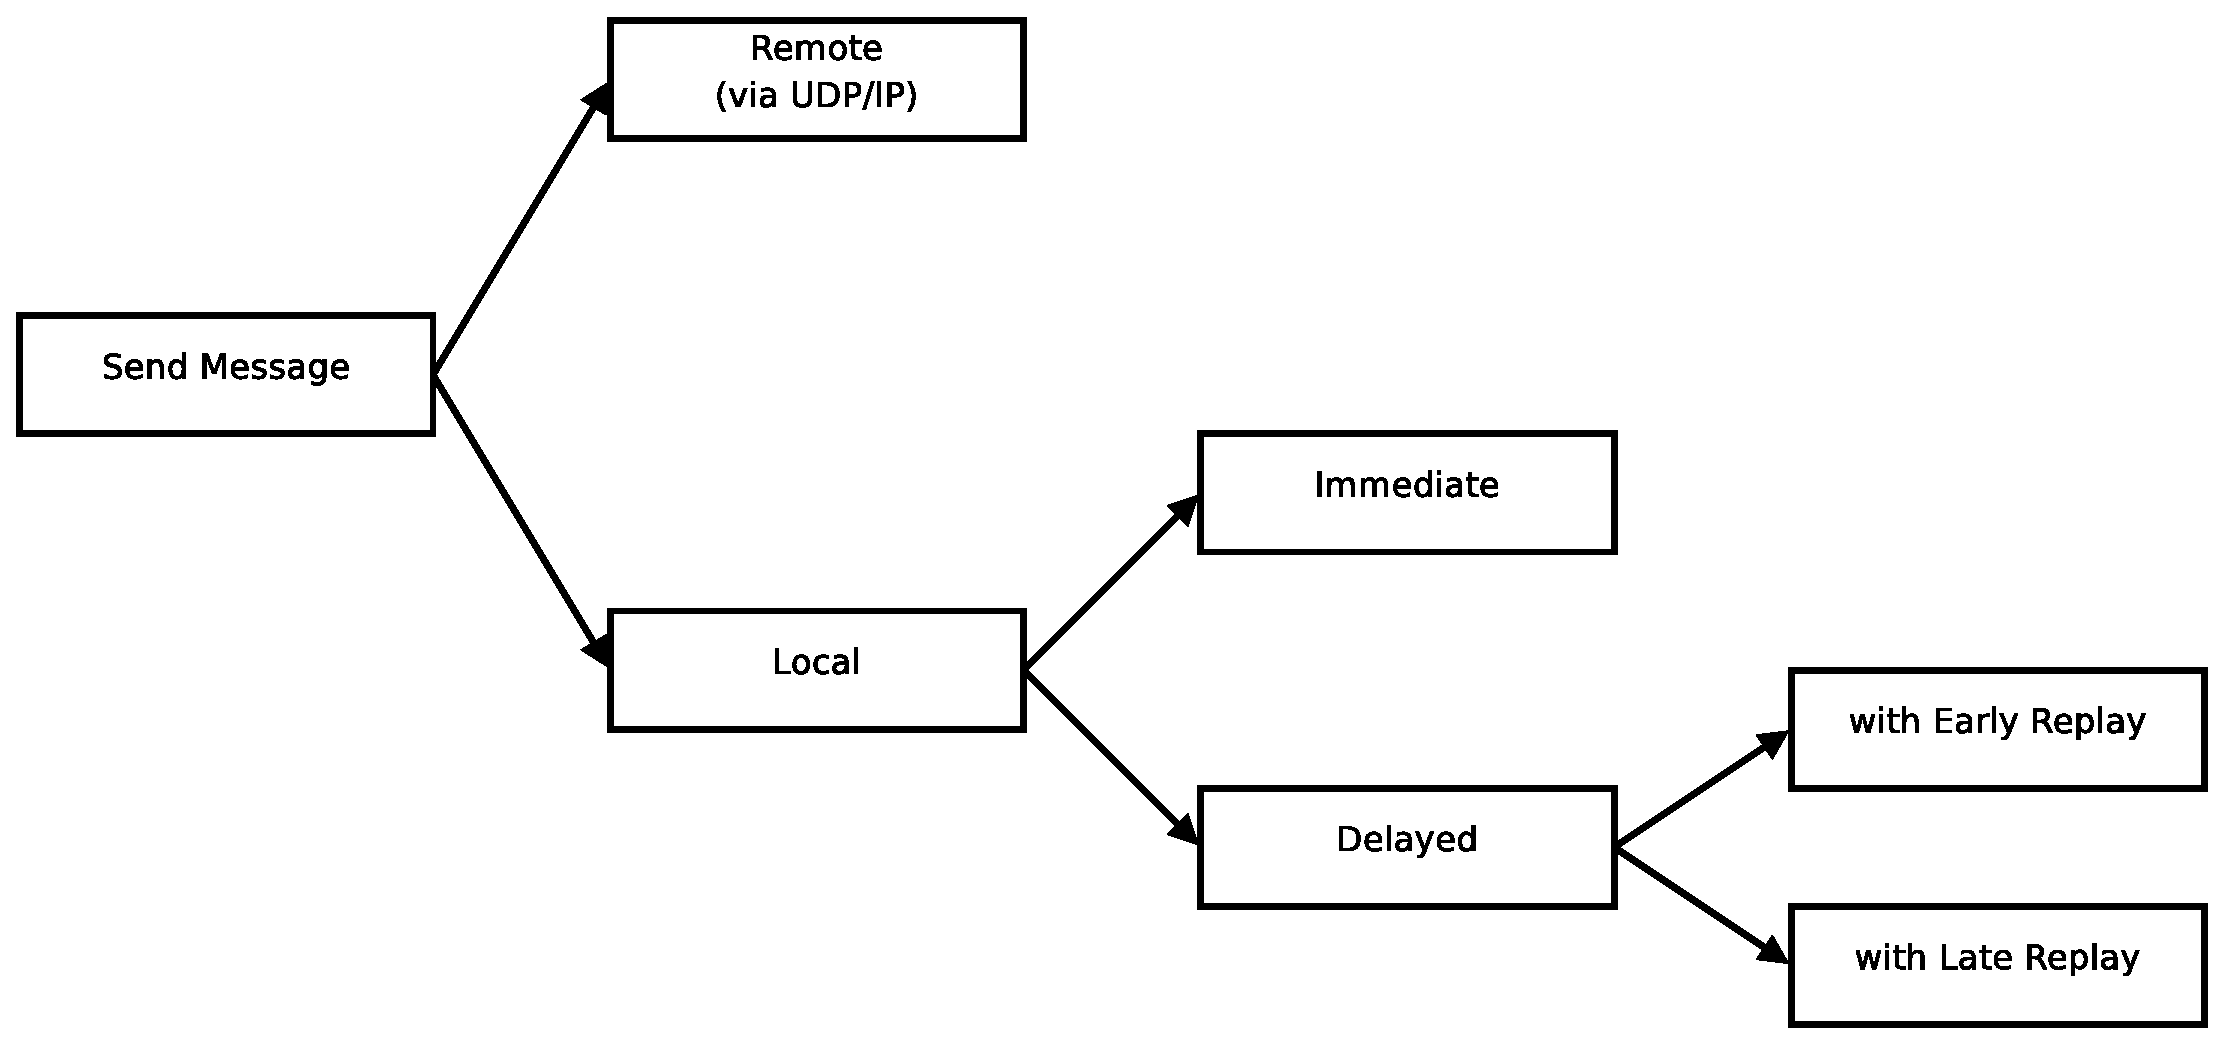
\includegraphics[width=0.66\textwidth]{level5/MessagesProp.eps} 
  \caption{BaseLib Level 5 messages properties diagram}
  \label{f:level5:MSGprop}
 \end{center}
\end{figure}


Using UDP/IP the policy for remote messages handling is to be Real Time, if it arrives it's ok otherwise doesn't mind, the timeout will save you.

Every message can be build up of any object type, a message is a list of objects that can also be a message itself. The whole UML diagram is depicted in Figure \ref{f:level5:MSG} and classes involved in this section are:
\begin{itemize}
 \item MessageCode
 \item Message

 \item MessageQueue
 \item MessageInterface
 \item MessageHandler

 \item MDRFlags
 \item MessageEnvelope
 \item MessageDeliveryRequest

 \item MessageDispatcher
 \item MessageBroker
 \item StartStopMessageHandlerInterface
 \item MessageServer
\end{itemize}

A \texttt{MessageCode} is an integer code that let comparing messages on the base of it; otherwise a message can be distingued from a string that is holded by the \texttt{Message} class.

Basically the vital work is done by the \texttt{MessageHandler} class that depends by the \texttt{MessageQueue} that holds messages that can be dispatched not immediately and by the \texttt{MessageInterface} that require the implementation of the two processing methods for the messages. \\
\begin{figure}[h!]
 \begin{center}
  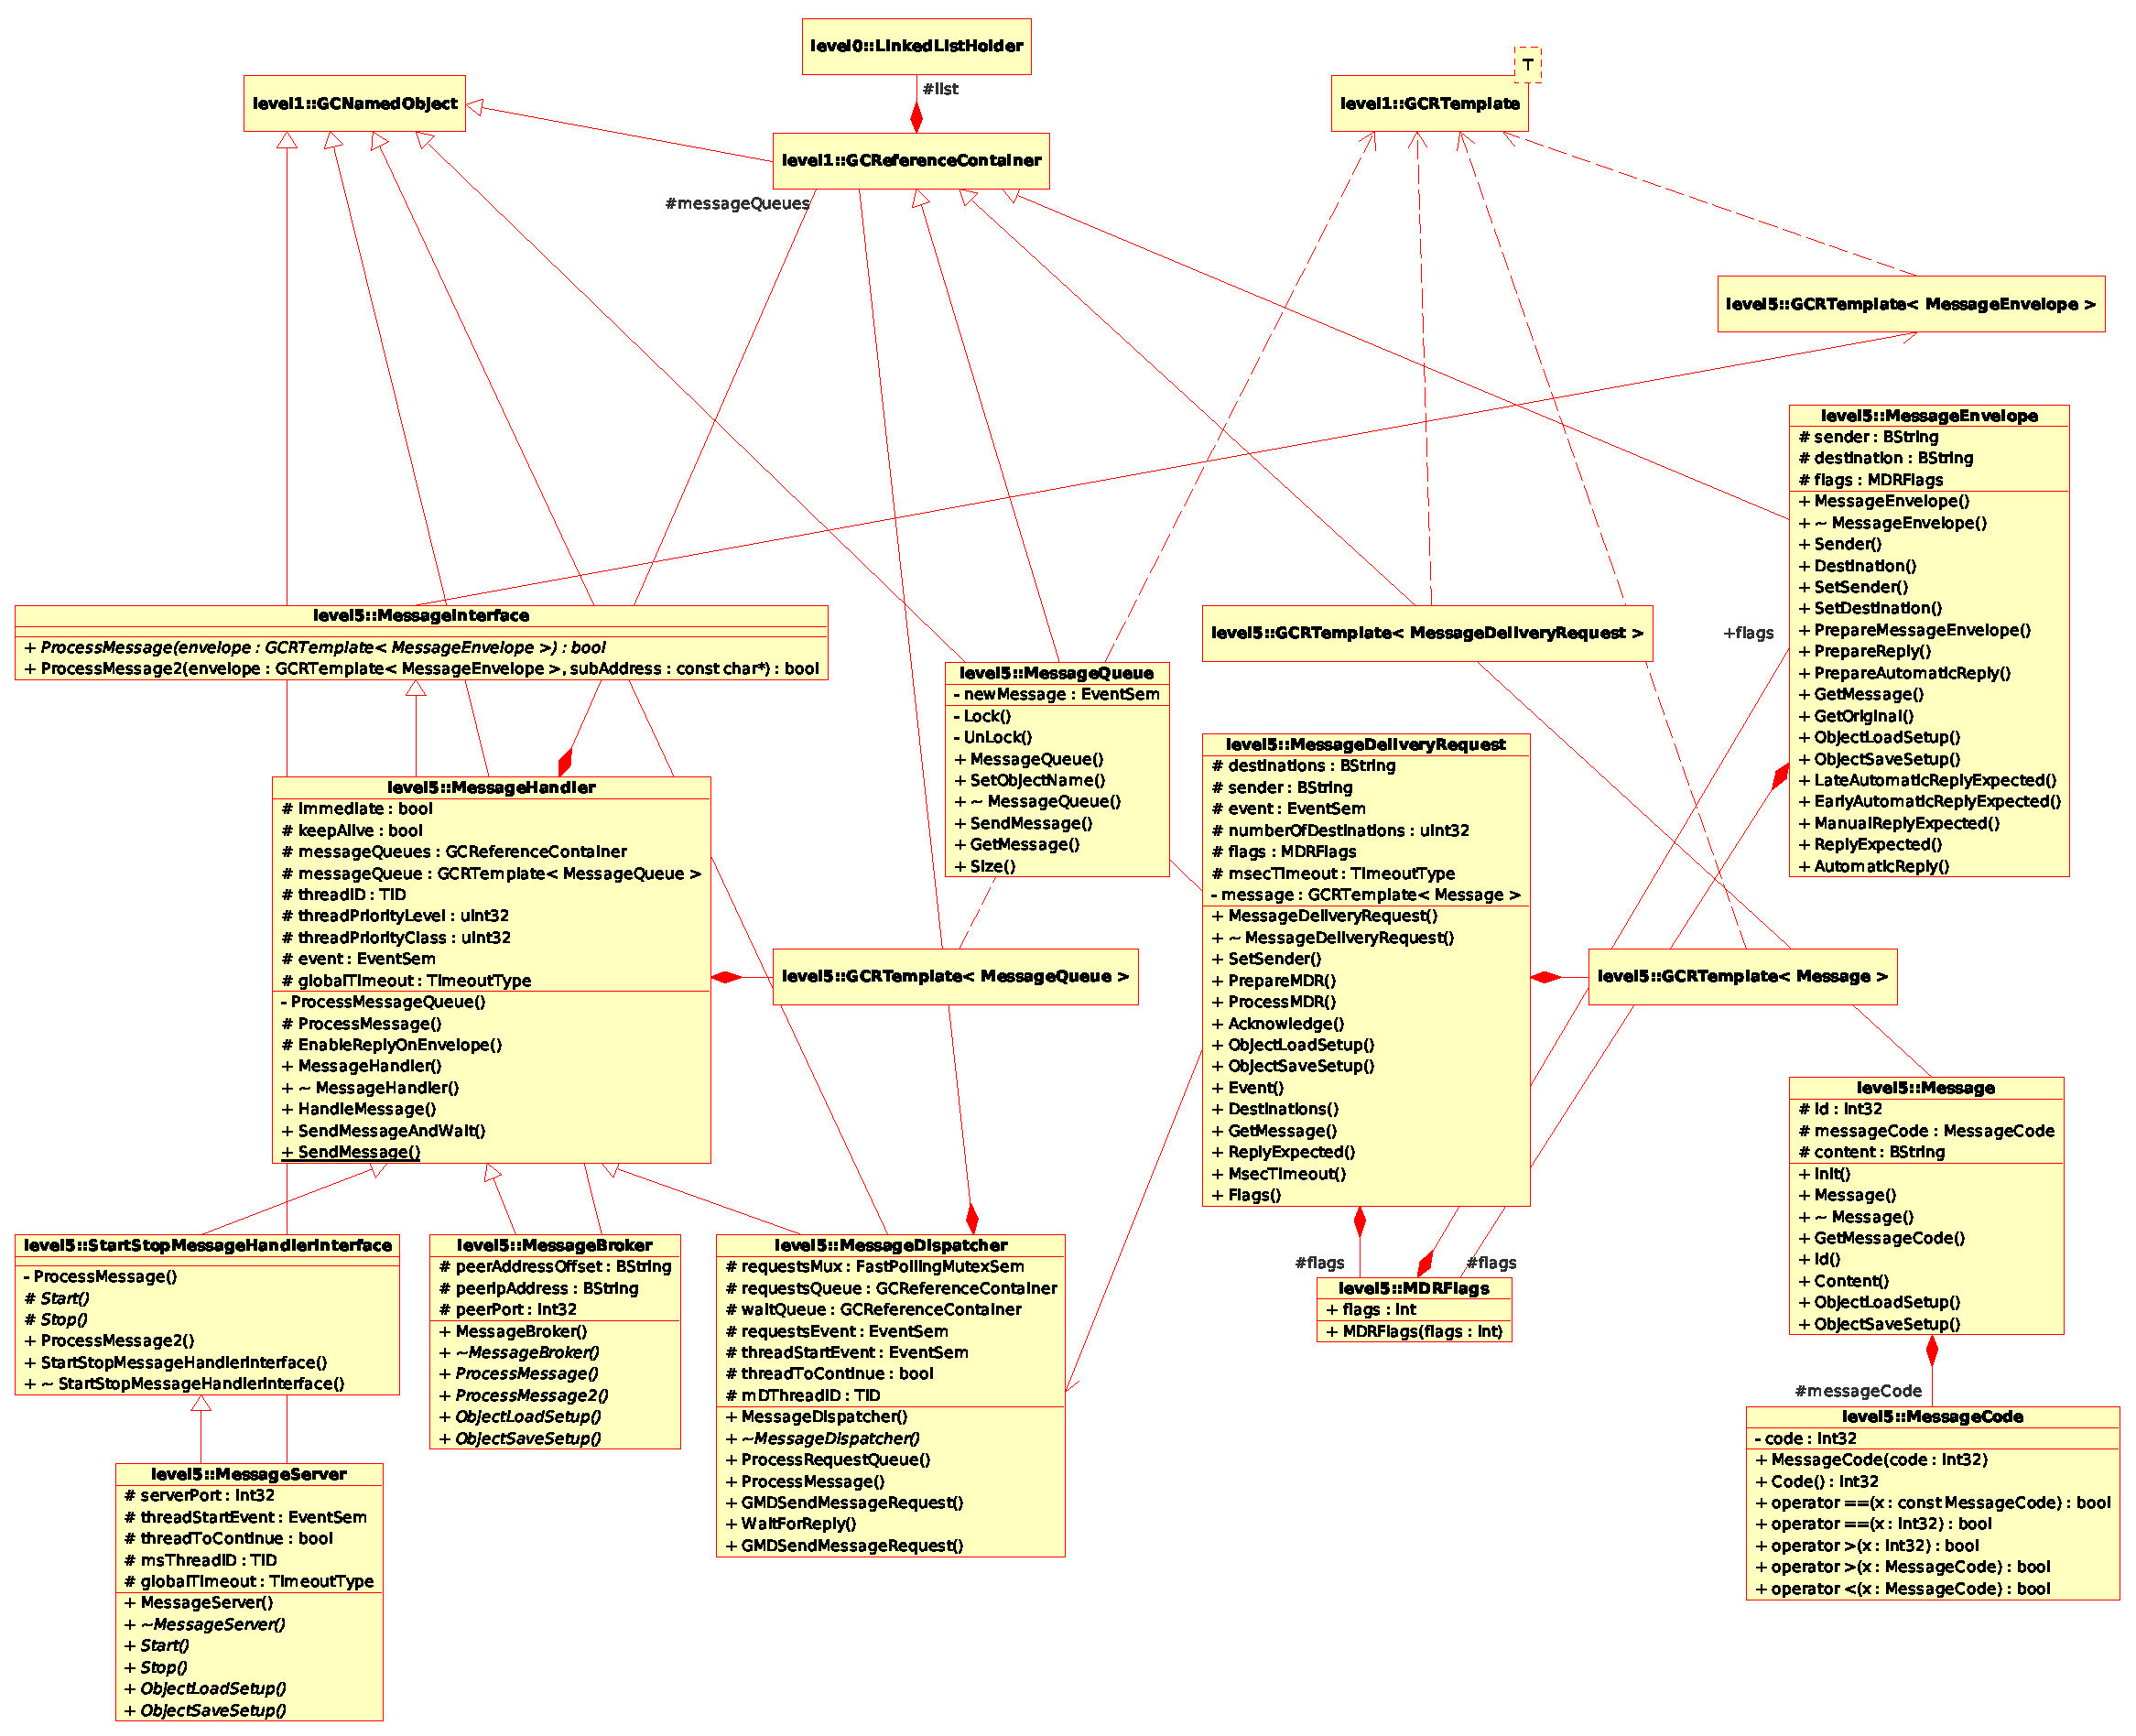
\includegraphics[width=1.1\textwidth]{level5/level5-MSG-exp.eps} 
  \caption{BaseLib Level 5 Messages}
  \label{f:level5:MSG}
 \end{center}
\end{figure}

The main method to send messages is the static \texttt{MessageHandler::SendMessage()}. This method is static so it is freely callable by any other classes that doesn't know how to send; if a class need a reply must extends the class \texttt{MessageHandler} or one of its subclasses. Any class that is a destination of a message must extend \texttt{MessageHandler}, and like before, or one of its subclasses. \\


Figure \ref{f:level5:MSG-dispatch} is an UML activity diagram that depict the steps for sending a message thorught the message infrastructure; some comments are needed. To send a message, the message must be first created, so a new \texttt{Message} class must be instantiated and a \texttt{MessageEnvelope} must be setted up with the source object pointer and the name of the destination class; the final destination class must be a \texttt{MessageHandler} subclass, otherwise it can not receive the message. We write ``final destination class'' because a destiantion address can be a dotted separated address of class names, i.e. the message can be sended between classes in a serial way, this is usefull for example in cases when you need to communicate to a remote class in another machine. An example of a remote location can be ``messageBroker.synchronizationGAM'' or ``(@192.168.2.3:1234).synchronizationGAM''. \\


After creating a \texttt{MessageEnvelope} it is possible to send it via the static \texttt{SendMessage} method; the first thing that is done is to check if it is a valid object, then the address is checked to know if it is a remote or a local message. If it is a remote message the \texttt{Message} is serialized and an UDP/IP socket is opened and the serialized object is sended.

If the message is local the first things that is done is to check against existance of the receiver object, if it exists in the GODB (the global registry of objects), it will be checked if it is of type \texttt{MessageHandler} otherwise the function returns with an error, infact if the receiver is not a \texttt{MessageHandler} subclass the message can not be delivered furthermore.

If the classes is founded then the control of the message is passed to class's methods, the first thing is to check against the form of dispatching, if it is \textit{immediate} the class's \texttt{ProcessMessage2} is called, otherwise a detached thread is made running and the message is queued for dispatching and the method returns.

\begin{sidewaysfigure}[h!]
 \centering
 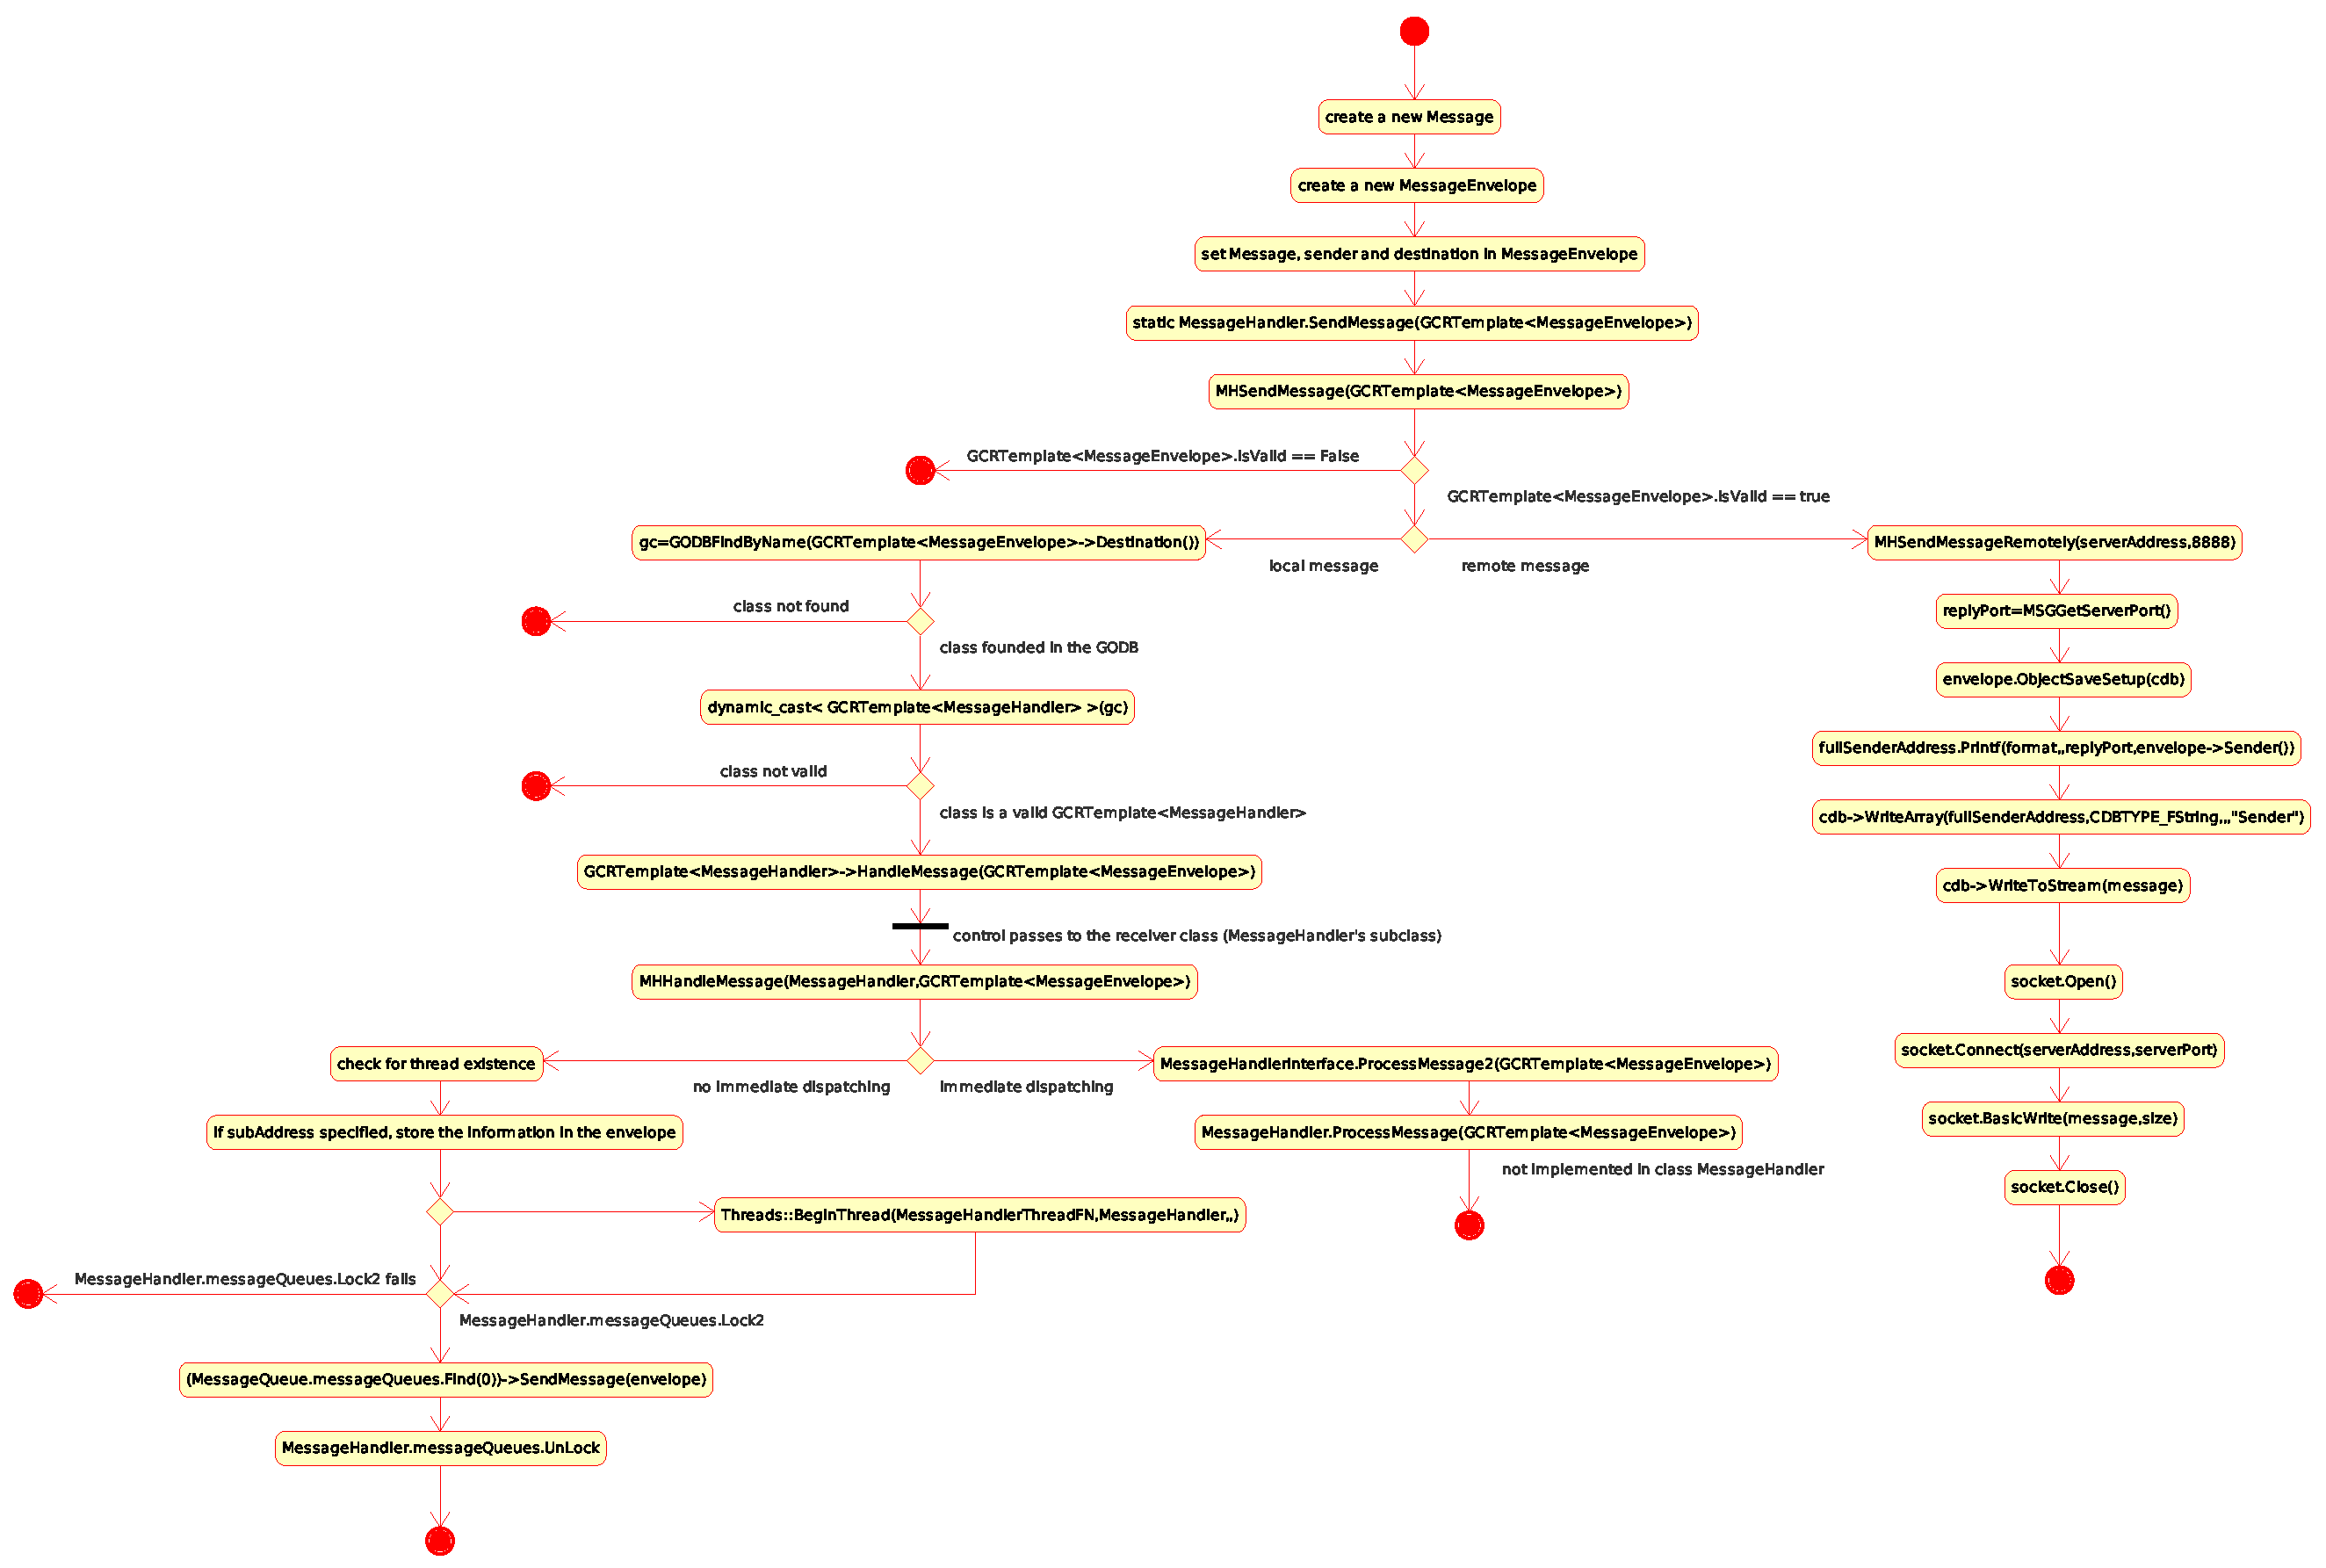
\includegraphics[width=\textwidth]{level5/MSG-dispatching.eps}
 \caption{BaseLib Level 5 \texttt{static MessageHandler::SendMessage()}}
 \label{f:level5:MSG-dispatch}
\end{sidewaysfigure}
\clearpage



The detached thread is a \texttt{MessageHandlerThreadFN}, refer to Figure \ref{f:level5:MSG-ThreadFN}, this thread is an asynchronous entity that delivers messages queued on the object. For each message an early reply and a late reply can be requested, the early reply is a message sended before the action of calling the \texttt{ProcessMessage2} method and the late reply after. There is a special treatment for \texttt{MenuMessage}s.

\begin{figure}[h!]
 \begin{center}
  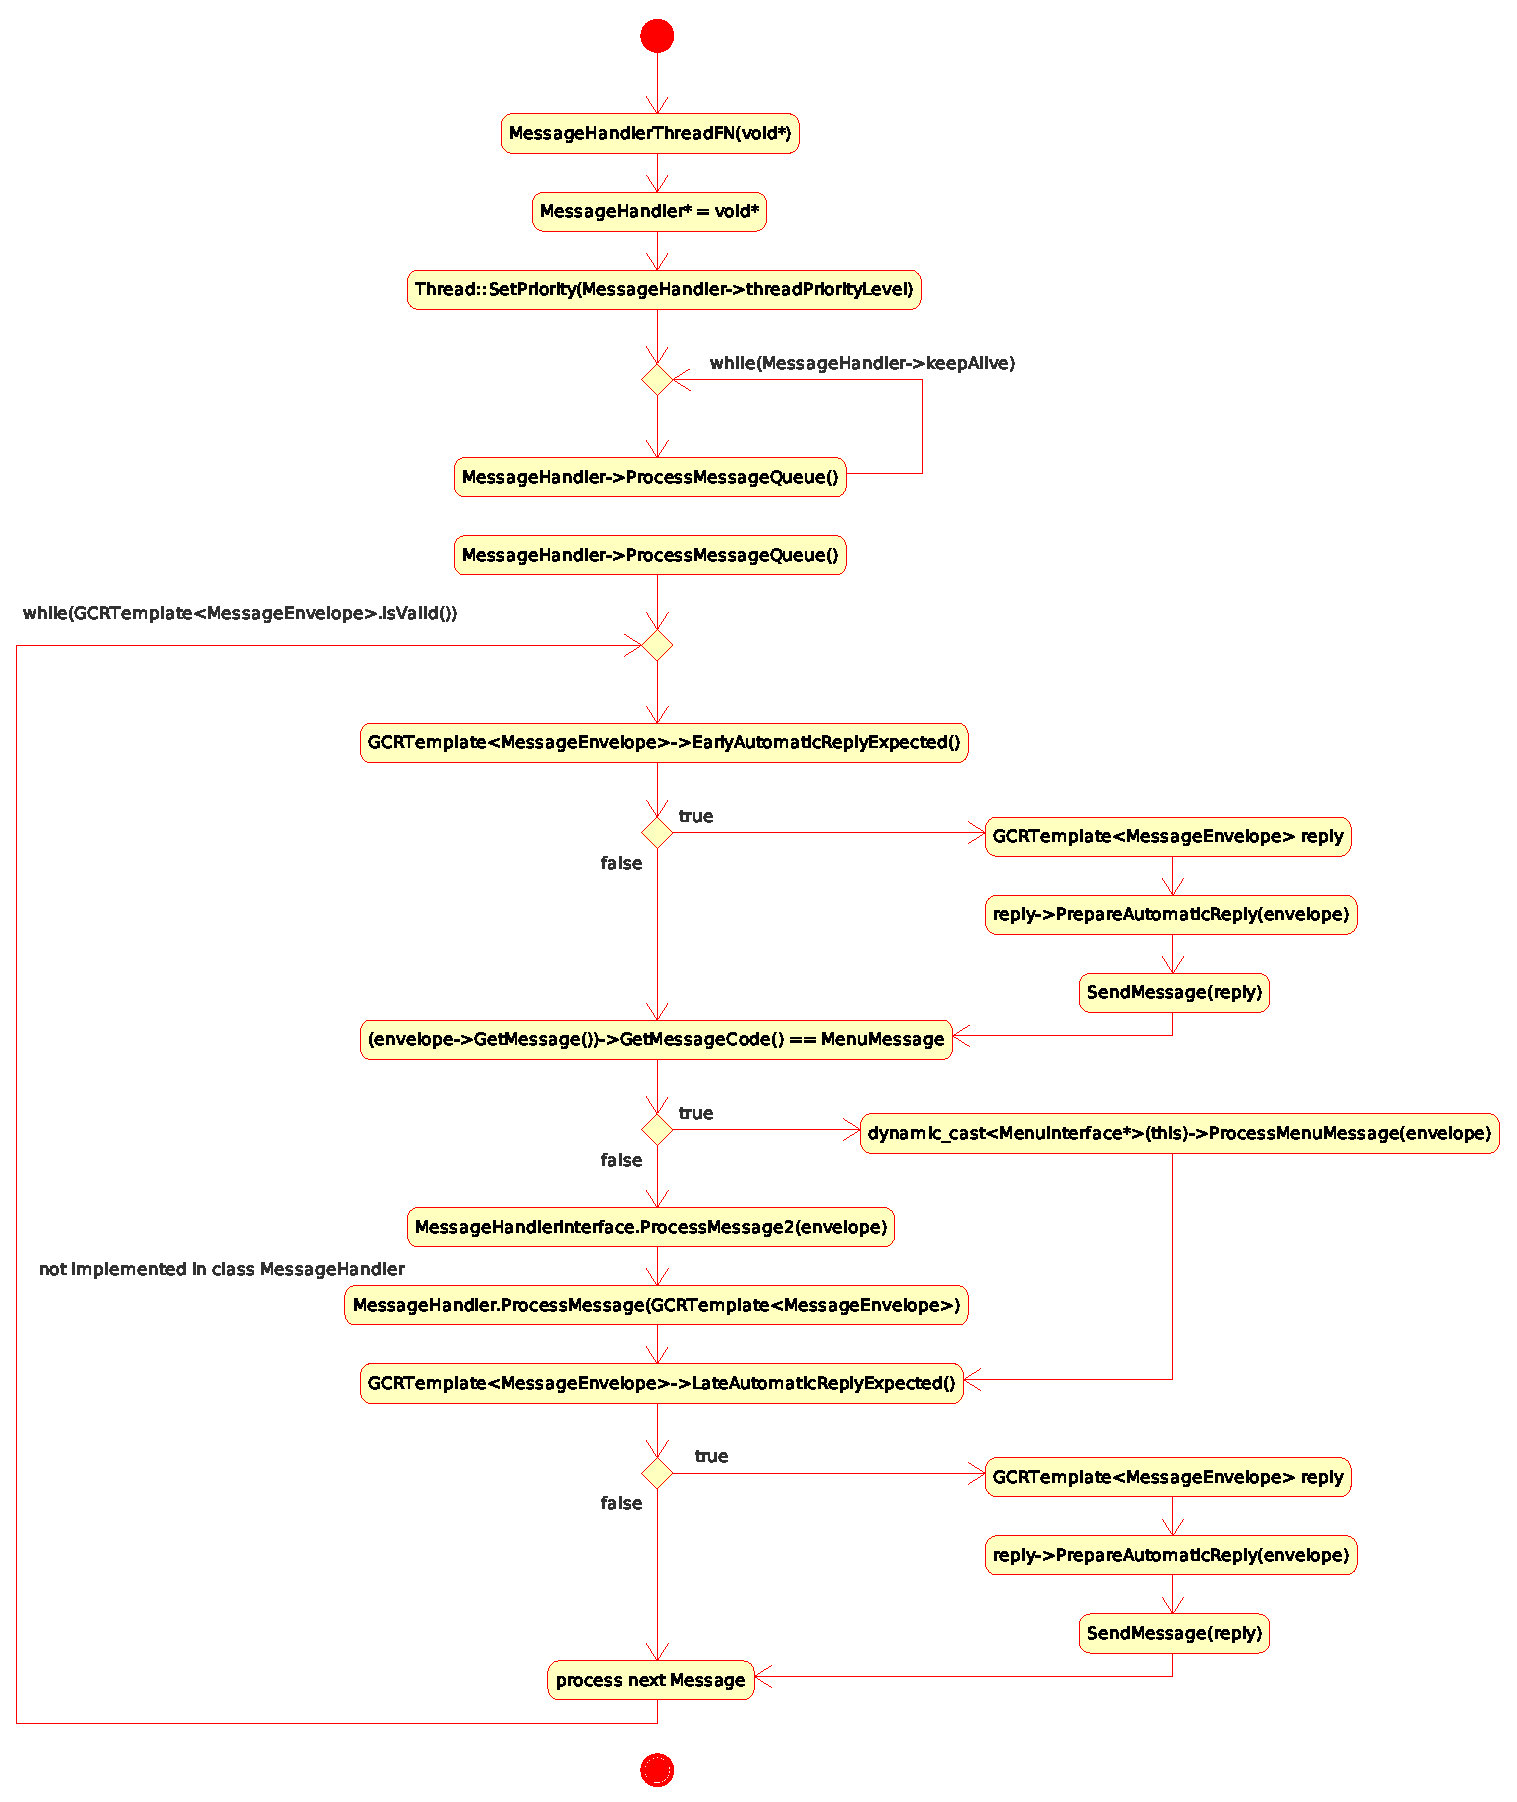
\includegraphics[width=0.77\textwidth]{level5/MSG-ThreadFN.eps} 
  \caption{BaseLib Level 5 \texttt{MessageHandlerThreadFN}}
  \label{f:level5:MSG-ThreadFN}
 \end{center}
\end{figure}



\subsubsection{MessageCode}
\texttt{[MessageCode.h]}\\
The class \texttt{MessageCode} implements the codes of the messages and some already defined codes. Such class is used to describe the content of a message, is just an integer but it enforces type checks. User defined \texttt{MessageCode}s starts from \texttt{UserMessageCode} (defined in the following). \\


As before the unique attribute is an \texttt{int32} that define the code itself. The constructor creates a new \texttt{MessageCode} object with the code passed by argument. \texttt{Code} accesses the \texttt{code} attribute. Then a set of operator redefinitions comes that are able to compare between message codes.
\begin{lstlisting}[
extendedchars=true,%
basicstyle=\fontfamily{pcr}\fontseries{m}\selectfont\footnotesize, %
stepnumber=1,%
numberstyle=\tiny,%
keywordstyle=\footnotesize\tt ,%
language=C++]
private:
   int32 code;

public:
   MessageCode(int32 code);
   inline int32 Code() const;

   inline bool operator==(const MessageCode x) const;
   inline bool operator==(int32 x) const;
   inline bool operator>(int32 x) const;
   inline bool operator>(MessageCode x) const;
   inline bool operator<(MessageCode x) const
\end{lstlisting}

The following message codes are statically defined in the \textit{level5/MessageCode.h} file. Each file that include \textit{MessageCode.h} has a local copy of these objects. Is a waste of space.

\begin{table}[!h]
 \begin{center}
  \begin{tabular}{|l|l|l|}
   \hline
description & object name & \texttt{int32 code} \\
    \hline
message rejected by the original recipient & \texttt{RejectedMessage} & \texttt{0xFFFFFFFF} \\
used when there is nothing to say & \texttt{NullMessage} & \texttt{0x0000} \\
standard reply to fully acknowledge a message & \texttt{FinishedMessage} & \texttt{0x0001} \\
a message directed to a \texttt{MenuInterface} & \texttt{MenuMessage} & \texttt{0x1001} \\
a message directed to a \texttt{HttpInterface} & \texttt{HttpMessage} & \texttt{0x1002} \\
first user defined message & \texttt{UserMessageCode} & \texttt{0x100000} \\
how many user message codes & \texttt{MaxUserMessageCode} & \texttt{0x100000} \\
    \hline
    \end{tabular}
   \end{center}
  \caption{Level5 Message codes}
 \label{t:level5:MSGCode}
\end{table}

\texttt{RejectedMessage} is the result of a message rejected by the original recipient; \texttt{NullMessage} is an empty message used when there is nothing to say; \texttt{FinishedMessage} is returned when it has finished using the data in the original message, this is the standard reply to fully acknowledge a message. \texttt{MenuMessage} is a message directed to a \texttt{MenuInterface}, the message payload must contain an \texttt{OutputStream} object and possibly an \texttt{InputStream} one. Both must be streamable; \texttt{HttpMessage} is a message directed to a \texttt{HttpInterface}.



\subsubsection{Message}
\texttt{[Message.h, Message.cpp]}\\
The class \texttt{Message} is made up with an identification number, a code, a string and an object reference container thanks to the \texttt{GCReferenceContainer} that its inherits from. \\


The first attribute is an \texttt{int32}, i.e. a system unique message identification, \texttt{messageCode} is a message code of the object and \texttt{content} is the message string. \\

The \texttt{Init} method sets the \texttt{messageCode} and \texttt{content} attributes. The constructor that is coming sets the \texttt{messageCode} to zero and \texttt{content} to a zero length string and \texttt{id} using the function \texttt{MSGGetUniqueId}. \texttt{GetMessageCode} retrieves the message code as a \texttt{MessageCode} object; \texttt{Id} retrieves the message \texttt{id}; \texttt{Content} retrieves the message \texttt{content}. \\

\noindent \texttt{ObjectLoadSetup} initialises an object from a set of configs, the syntax is:
\begin{table}[!h]
  \begin{tabular}{l}
\texttt{Code = <a number>} or in alternative \\
\texttt{UserCode = <a number>} in this case the code will be offsetted with \texttt{UserCode} index \\
\texttt{Content = <}any text (within " if includes spaces)\texttt{>} \\
or standard \texttt{GCReferenceContainer} syntax \\
  \end{tabular}
\end{table}

\noindent \texttt{ObjectSaveSetup} saves the object into a set of configs, the syntax is:
\begin{table}[!h]
  \begin{tabular}{l}
\texttt{Code = <a number>} \\
\texttt{Id = <a number>} \\
\texttt{Content = <}any text (within " if includes spaces)\texttt{>} \\
or standard \texttt{GCReferenceContainer} syntax \\
  \end{tabular}
\end{table}

\begin{lstlisting}[
extendedchars=true,%
basicstyle=\fontfamily{pcr}\fontseries{m}\selectfont\footnotesize, %
stepnumber=1,%
numberstyle=\tiny,%
keywordstyle=\footnotesize\tt ,%
language=C++]
protected:
   int32 id;
   MessageCode messageCode;
   BString content;

public:
   void Init(MessageCode code,const char* content);

   Message() :messageCode(0);
   virtual ~Message();

   MessageCode GetMessageCode();
   int32 Id();
   const char* Content();

   virtual bool ObjectLoadSetup(ConfigurationDataBase& info,StreamInterface* err);
   virtual bool ObjectSaveSetup(ConfigurationDataBase& info,StreamInterface* err);
\end{lstlisting}



\subsubsection{MessageQueue}
\texttt{[MessageQueue.h]}\\
A class \texttt{MessageQueue} is a \texttt{GCReferenceContainer} with a FIFO only policy and an \texttt{EventSem} to synchronise tasks to new data arrival. The \texttt{EventSem} wake up when a new message is in the queue.
The superclass \texttt{GCReferenceContainer} mantain a list (a queue) of \texttt{GCNamedObject}s and this class exploits this functionality. \\


Methods \texttt{Lock} and \texttt{UnLock} guarantees concurrent access to the objects. The constructor create the semaphore \texttt{newMessage} and the destructor destroyes it.
The method \texttt{SetObjectName} calls the \texttt{GCNamedObject::SetObjectName} via \texttt{GCReferenceContainer} class.
The method \texttt{SendMessage} enqueue a \texttt{GCRTemplate<MessageEnvelope>} object on the \texttt{GCReferenceContainer}'s linked list; \texttt{GetMessage} returns the oldest message queued in the linked list. \texttt{Size} return the number of elements in the linked list.
\begin{lstlisting}[
extendedchars=true,%
basicstyle=\fontfamily{pcr}\fontseries{m}\selectfont\footnotesize, %
stepnumber=1,%
numberstyle=\tiny,%
keywordstyle=\footnotesize\tt ,%
language=C++]
private:
   EventSem newMessage;

   bool Lock(TimeoutType tt = TTInfiniteWait);
   bool UnLock();

public:
   MessageQueue();
   virtual ~MessageQueue();

   void SetObjectName(const char* name);
   bool SendMessage(GCRTemplate<MessageEnvelope> envelope,TimeoutType tt=TTInfiniteWait);
   GCRTemplate<MessageEnvelope> GetMessage(TimeoutType tt=TTInfiniteWait);
   int32 Size();
\end{lstlisting}



\subsubsection{MessageInterface}
\texttt{[MessageInterface.h]}\\
The class \texttt{MessageInterface} is formally the interface that can be used to create multiple message handling objects. This interface alone cannot implement a \texttt{MessageHandler}; to implement an object with multiple message handling capabilities simply have each component class inherit from this class and then the final class inherit from all the base classes and \texttt{MessageHandler}.

If each component class has registered itself with the \texttt{MessageHandler} then the standard message handling function will try all the interfaces.

The methods to be implemented by the user application follows.

\begin{lstlisting}[
extendedchars=true,%
basicstyle=\fontfamily{pcr}\fontseries{m}\selectfont\footnotesize, %
stepnumber=1,%
numberstyle=\tiny,%
keywordstyle=\footnotesize\tt ,%
language=C++]
public:
   virtual bool ProcessMessage(GCRTemplate<MessageEnvelope> envelope)=0;
   virtual bool ProcessMessage2(GCRTemplate<MessageEnvelope> envelope,const char* subAddress);
\end{lstlisting}



\subsubsection{MessageHandler}
\texttt{[MessageHandler.h, MessageHandler.cpp]}\\
The class \texttt{MessageHandler} is the main class for subclassing objects that can handle messages.
Based on the \texttt{immediate} attribute the \texttt{MessageHandler} object will handle the message immediately or it will put the message on a queue and spawn a thread to handle it later. \\


We now take a look at the attributes of the class. The \texttt{immediate} attribute is \texttt{true} if the message is processed immediately; note that the user handler function must be able to handle parallel requests to work, in the following we speak about it. The attribute \texttt{keepAlive} says if is to keep the thread alive; \texttt{messageQueues} are the pools of queues and \texttt{messageQueue} is the local message queue. \\


The attribute \texttt{threadID} is the thread identification if not zero it means that a thread is running. \texttt{threadPriorityLevel} is the level at which the handler task operates; \texttt{threadPriorityClass} is the level at which the handler task operates, priority classes are:

\begin{table}[!h]
 \begin{center}
  \begin{tabular}{cl}
priority class & description \\
   \hline
0 & Idle \\
1 & Regular \\
2 & Server \\
3 & RT \\
  \end{tabular}
 \end{center}
\end{table}

\texttt{event} is a semaphore on which to wait for the task start/stop events and \texttt{globalTimeout} is how long to wait for single action.
\begin{lstlisting}[
extendedchars=true,%
basicstyle=\fontfamily{pcr}\fontseries{m}\selectfont\footnotesize, %
stepnumber=1,%
numberstyle=\tiny,%
keywordstyle=\footnotesize\tt ,%
language=C++]
protected:
   bool immediate;
   bool keepAlive;
   GCReferenceContainer messageQueues;
   GCRTemplate<MessageQueue> messageQueue;

   TID threadID;
   uint32 threadPriorityLevel;
   uint32 threadPriorityClass;

   EventSem event;
   TimeoutType globalTimeout;
\end{lstlisting}

The method \texttt{ProcessMessageQueue} is the actual body of the managing thread, method \texttt{ProcessMessage} must be overridden in descendent classes; \texttt{envelope} should be a valid reference to a \texttt{MessageEnvelope}, it returns \texttt{true} if the message is considered to have been consumed \texttt{false} if the handler does not recognise the message as its own, at this level it simply return \texttt{false}. \\

\texttt{EnableReplyOnEnvelope} if the envelope has no reply mechanism specified basically modify the \texttt{envelope::flags} attribute to \texttt{MDRF\_EarlyAutomaticReply} see more on next classes. \\


The constructor by default set the \texttt{immediate} attribute to \texttt{false} requiring the creation of a thread but in the constructor no thread is created and the priority level is sets to zero. The \texttt{gloablTimeout} is of about 1000ms, a queue is also created and is queued on the \texttt{messageQueues} attribute. The destructor try to destroy a living thread that handle the queues completion if it exists. \\


The method \texttt{HandleMessage} is the function to be called to handle the message, so it must be written to be able to handle parallel requests. Such method calls the \texttt{ProcessMessage} method if is a local message.
\texttt{SendMessageAndWait} sends a message and wait for reply; the last function \texttt{SendMessage}, is the only function that sends a message by any other class.
\begin{lstlisting}[
extendedchars=true,%
basicstyle=\fontfamily{pcr}\fontseries{m}\selectfont\footnotesize, %
stepnumber=1,%
numberstyle=\tiny,%
keywordstyle=\footnotesize\tt ,%
language=C++]
private:
   void ProcessMessageQueue();
protected:
   virtual bool ProcessMessage(GCRTemplate<MessageEnvelope> envelope);

   void EnableReplyOnEnvelope(GCRTemplate<MessageEnvelope> envelope);
public:
   MessageHandler();
   virtual ~MessageHandler();

   inline  bool HandleMessage(GCRTemplate<MessageEnvelope> envelope,
      const char* subAddress = NULL);

   inline bool SendMessageAndWait(GCRTemplate<MessageEnvelope> envelope,
      GCRTemplate<MessageEnvelope>&  reply,TimeoutType timeout=TTInfiniteWait);
   static inline bool  SendMessage(GCRTemplate<MessageEnvelope> gcrtme);
\end{lstlisting}



\subsubsection{MDRFlags}
\texttt{[MDRFlags.h]}\\
The \texttt{MDRFlags} class, i.e. Message Delivery Request Flags, is used to control \texttt{MessageEnvelope} and \texttt{MessageDeliveryRequest}. The class follows and is made by only one attribute and no methods.

\begin{lstlisting}[
extendedchars=true,%
basicstyle=\fontfamily{pcr}\fontseries{m}\selectfont\footnotesize, %
stepnumber=1,%
numberstyle=\tiny,%
keywordstyle=\footnotesize\tt ,%
language=C++]
class MDRFlags {
public:
   int flags;
};
\end{lstlisting}

\texttt{MDRFlags} global objects are:

\begin{table}[!h]
 \begin{center}
  \begin{tabular}{|l|l|l|}
   \hline
description & object name & \texttt{int flags} \\
   \hline
no flags & \texttt{MDRF\_None} & \texttt{0x0000} \\
no flags & \texttt{MDRF\_ReplyMask} & \texttt{0x0003} \\
no flags & \texttt{MDRF\_ReplyNMask} & \texttt{0xFFFFFFFC} \\
Create a reply soon before or after user & \texttt{MDRF\_AutomaticReply} & \texttt{0x0001} \\
Create a reply after or as part of user & \texttt{MDRF\_LateReply} & \texttt{0x0002} \\
Create a reply soon before user & \texttt{MDRF\_EarlyAutomaticReply} & \texttt{0x0001} \\
Create a reply soon after user & \texttt{MDRF\_LateAutomaticReply} & \texttt{0x0003} \\
No reply generated or expected & \texttt{MDRF\_NoReply} & \texttt{0x000} \\
Manual reply expected & \texttt{MDRF\_ManualReply} & \texttt{0x0002} \\
Mask to check for any form of replya expected & \texttt{MDRF\_ReplyExpected} & \texttt{0x003} \\
allows using partialName in address & \texttt{MDRF\_MatchPartialName} & \texttt{0x0004} \\
This is a reply with no new message & \texttt{MDRF\_Reply} & \texttt{0x10000} \\
    \hline
    \end{tabular}
   \end{center}
  \caption{Level5 Message Delivery Request flags}
 \label{t:level5:MDRFlags}
\end{table}



\subsubsection{MessageEnvelope}
\texttt{[MessageEnvelope.h, MessageEnvelope.cpp]}\\
The class \texttt{MessageEnvelope} is a folder containing one or more \texttt{Message} objects (due to inherit from \texttt{GCReferenceContainer}), the destination and sender object's address and possibly the mail it was replying to. The destination and sender object's address are strings (BString attribute \texttt{sender} and \texttt{destination}) so destination and sender objects must be searched by name. \\


The constructor builds an empty envelope setting \texttt{sender} and \texttt{destination} to \texttt{``none''}. The method \texttt{Sender} retrieves the message sender, \texttt{Destination} retrieves the message destination; \texttt{SetSender} sets the specified object as the sender of the message, note that you must use an \texttt{GCNamedObject} as a sender, i.e. must be an object with a name; \texttt{SetDestination} sets the specified object as the destination of a message, the destination object is not checked against existance in this method.
\begin{lstlisting}[
extendedchars=true,%
basicstyle=\fontfamily{pcr}\fontseries{m}\selectfont\footnotesize, %
stepnumber=1,%
numberstyle=\tiny,%
keywordstyle=\footnotesize\tt ,%
language=C++]
protected:
   BString sender;
   BString destination;
   MDRFlags flags;

public:
   MessageEnvelope();
   virtual ~MessageEnvelope();

   inline const char* Sender();
   inline const char* Destination();
   inline void SetSender(GCNamedObject& sender);
   inline void SetDestination(const char* destination);
\end{lstlisting}

The method \texttt{PrepareMessageEnvelope} adds the \texttt{message} passed by argument to the \texttt{GCReferenceContainer} list using \texttt{GCReferenceContainer::Insert} method and sets \texttt{sender}, \texttt{destination} and \texttt{flags} attributes; if \texttt{destination} starts with \texttt{::} the name search scope is the global object container otherwise it is the message receiver container; use \texttt{flags} to request a reply.

The method \texttt{PrepareReply} creates a \texttt{MessageEnvelope} as a reply to the \texttt{MessageEnvelope}, swaps sender and destination and copies all content; \texttt{maxHistory} regulates the number of old-messages left in the envelope.

The method \texttt{PrepareAutomaticReply} is the acknowledge to a message reception; it is automatically generated from the original enevelope, message's \texttt{flags} is \texttt{MDRF\_Reply}.\\


The method \texttt{GetMessage} returns the first message in the envelope that can hold more then one message, it uses \texttt{GCReferenceContainer::Find}. \texttt{GetOriginal} gets the original message if this is a reply, \texttt{index} default \texttt{1} is the original message any higher number is the history of messages.\\


The usual \texttt{ObjectLoadSetup} initialises an object from a set of configs, the syntax is:
\begin{lstlisting}[
extendedchars=true,%
basicstyle=\fontfamily{pcr}\fontseries{m}\selectfont\footnotesize, %
stepnumber=1,%
numberstyle=\tiny,%
keywordstyle=\footnotesize\tt ,%
language=bash]
Sender = <any text (within "" if includes spaces) >
Destination = <any text (within "" if includes spaces) >
<Use syantax of GCReferenceContainer>
Add = {
    MessageName = {
      <See Message syntax>
    }
    [ReplyName = {
       <See Message syntax>
    }]
}
\end{lstlisting}
\texttt{ObjectSaveSetup} saves an object to a set of configs; the syntax is:
\begin{lstlisting}[
extendedchars=true,%
basicstyle=\fontfamily{pcr}\fontseries{m}\selectfont\footnotesize, %
stepnumber=1,%
numberstyle=\tiny,%
keywordstyle=\footnotesize\tt ,%
language=bash]
Sender = <any text (within "" if includes spaces) >
Destination = <any text (within "" if includes spaces) >
Content = {
        <Use syantax of GCReferenceContainer>
        Add = {
          Message = {
            <See Message syntax>
          }
          [Reply = {
             <See Message syntax>
          }]
        }
        ... (other message names are possible)
}
\end{lstlisting}
 
The following methods simply tests for if the \texttt{flags} attribute has a particular value. \texttt{LateAutomaticReplyExpected} is \texttt{true} if an automatic reply shall be generated after processing, \texttt{EarlyAutomaticReplyExpected} is \texttt{true} if an automatic reply shall be generated, \texttt{ManualReplyExpected} is \texttt{true} if a manual reply shall be generated by the user, \texttt{ReplyExpected} is \texttt{true} if a manual reply shall be generated by the user and \texttt{AutomaticReply} is \texttt{true} if an automatic reply.

\begin{lstlisting}[
extendedchars=true,%
basicstyle=\fontfamily{pcr}\fontseries{m}\selectfont\footnotesize, %
stepnumber=1,%
numberstyle=\tiny,%
keywordstyle=\footnotesize\tt ,%
language=C++]
   inline bool PrepareMessageEnvelope(GCRTemplate<Message> message,
      const char* destination,MDRFlags flags=MDRF_None,GCNamedObject* source=NULL);
   inline bool PrepareReply(GCRTemplate<MessageEnvelope> messageEnvelope,
      GCRTemplate<Message> replyMessage,MDRFlags flags=MDRF_None,int maxHistory=2);
   inline bool PrepareAutomaticReply(GCRTemplate<MessageEnvelope> envelope);

   inline GCRTemplate<Message> GetMessage();
   inline GCRTemplate<Message> GetOriginal(int index=1);

   virtual bool ObjectLoadSetup(ConfigurationDataBase& info,StreamInterface* err);
   virtual bool ObjectSaveSetup(ConfigurationDataBase& info,StreamInterface* err);

   inline bool LateAutomaticReplyExpected() const;
   inline bool EarlyAutomaticReplyExpected() const;
   inline bool ManualReplyExpected() const;
   inline bool ReplyExpected() const;
   inline bool AutomaticReply() const;
\end{lstlisting}



\subsubsection{MessageDeliveryRequest}
\texttt{[MessageDeliveryRequest.h, MessageDeliveryRequest.cpp]}\\
The class \texttt{MessageDeliveryRequest} is a container that will hold a message and associated data; the class holds a sender reference, a list of recipients and a mechanism to synchronise a sender with the return receipts from all its recipients. The class \texttt{MessageDeliveryRequest} inherits from \texttt{GCNamedObject}. \\


Attributes are all protected, there is an explicit \texttt{GCRTemplate<Message>} attribute that holds a \texttt{Message} objects via templatization. \texttt{sender} is who made the request; \texttt{destination} is a comma/space separated list of destinations and \texttt{nuberOfDestinations} is the number of valid destinations created when sending messages by \texttt{ProcessMDR}. The attribute \texttt{event} is a sempahore on wich to wait for reply at least \texttt{msecTimeout} milliseconds; other options are stored in \texttt{flags}.
\begin{lstlisting}[
extendedchars=true,%
basicstyle=\fontfamily{pcr}\fontseries{m}\selectfont\footnotesize, %
stepnumber=1,%
numberstyle=\tiny,%
keywordstyle=\footnotesize\tt ,%
language=C++]
protected:
   GCRTemplate<Message> message;

   BString sender;
   BString destinations;
   uint32 numberOfDestinations;

   EventSem event;
   TimeoutType msecTimeout;
   MDRFlags flags;
\end{lstlisting}

The constructor builds an empty request with zero destinations and inifinte timeout creting also the semaphore; the destructor simply delete the semaphore. \texttt{SetSender} sets the specified object as sender of the message, like \texttt{MessageEnvelope} should be a \texttt{GCNamdeObject}.\\

The method \texttt{PrepareMDR} sets all the arguments passed by to the attributes in the class; the message is saved in the \texttt{message} attribute. \texttt{ProcessMDR} prepares envelopes and delivers them, the delivery is done via the \texttt{MessageHandler::SendMessage} static method for each destination in the \texttt{destinations} attribute. \texttt{Acknowledge} counts down the number of messages to acknowledge, returns \texttt{true} only when all acks are received. \\


The method \texttt{ObjectLoadSetup} initialises an object from a set of configs; the syntax is (the object name is taken from the current node name):
\begin{lstlisting}[
extendedchars=true,%
basicstyle=\fontfamily{pcr}\fontseries{m}\selectfont\footnotesize, %
stepnumber=1,%
numberstyle=\tiny,%
keywordstyle=\footnotesize\tt ,%
language=bash]
Sender = <any text (within "" if includes spaces) >
Destinations = <any text (within "" if includes spaces)
               multiple destinations are space or comma separated >
MsecTimeOut = how msec to wait for reply
Flags = [ EarlyAutomaticReply LateAutomaticReply NoReply ManualReply ]
Message = {
  Class = Message
  <See Message syntax>
}
\end{lstlisting}

\texttt{ObjectSaveSetup} saves an object to a set of configs; the syntax is as follows:
\begin{lstlisting}[
extendedchars=true,%
basicstyle=\fontfamily{pcr}\fontseries{m}\selectfont\footnotesize, %
stepnumber=1,%
numberstyle=\tiny,%
keywordstyle=\footnotesize\tt ,%
language=bash]
Sender = <any text (within "" if includes spaces) >
Destinations = <any text (within "" if includes spaces) >
Message = {
  Class = Message
  <See Message syntax>
}
\end{lstlisting}

\texttt{Event} returns \texttt{event} attribute, \texttt{Destinations} returns the destinations string and \texttt{GetMessage} returns the message.

\texttt{Flags} returns \texttt{flags} attribute, \texttt{ReplyExpected} is \texttt{true} if we want wait for reply, \texttt{MsecTimeout} is how long to wait for a reply.
\begin{lstlisting}[
extendedchars=true,%
basicstyle=\fontfamily{pcr}\fontseries{m}\selectfont\footnotesize, %
stepnumber=1,%
numberstyle=\tiny,%
keywordstyle=\footnotesize\tt ,%
language=C++]
public:
   MessageDeliveryRequest();
   ~MessageDeliveryRequest();

   inline void SetSender(GCNamedObject& sender);

   inline bool PrepareMDR(GCRTemplate<Message> message,
      const char* destinations,MDRFlags flags=MDRF_None,
      GCNamedObject* source=NULL,TimeoutType msecTimeout=TTInfiniteWait);
   bool ProcessMDR(MessageDispatcher *md);
   bool Acknowledge();

   virtual bool ObjectLoadSetup(ConfigurationDataBase& info,StreamInterface* err);
   virtual bool ObjectSaveSetup(ConfigurationDataBase& info,StreamInterface* err);
   
   inline EventSem& Event();
   inline const char* Destinations() const;
   inline GCRTemplate<Message> GetMessage() const;

   inline MDRFlags Flags() const;
   inline bool ReplyExpected() const;
   inline TimeoutType MsecTimeout() const;
\end{lstlisting}



\subsubsection{MessageDispatcher}
\texttt{[MessageDispatcher.h, MessageDispatcher.cpp]}\\
The class \texttt{MessageDispatcher} is a special global object that handles sending messages for third parties. Those class provide message sending to single/multiple recipients; provides also wait for acknowledge service from single/multiple destinations. Such class is teh first of the three implementations of the \texttt{ProcessMessage} method in this level (in \texttt{MessageHandler} and in \texttt{MessageInterface} simply return \texttt{false} or is not implemented).

It inherits from \texttt{GCNamedObject} and \texttt{MessageHandler}. There is a globally declared object \texttt{globalMessageDispatcher} that formally is a \texttt{GCRTemplate<MessageDispatcher>} and is returned by the global function \texttt{GlobalMessageDispatcher()} in \textit{level5/MessageDispatcher.cpp}. \\


The first attribute, \texttt{requestMux} protects access to the \texttt{requestsQueue} attribute that is the next argument. \texttt{waitQueue} is the queue of elements to be acknowledge. The semaphore \texttt{requestsEvent} is used to mark a new request in the list, \texttt{threadStartEvent} to mark the start of the handling thread, the boolean \texttt{threadToContinue} requests the end of the processing thread, \texttt{mDThreadID} is the thread identifier, if not zero it means a thread is running.
\begin{lstlisting}[
extendedchars=true,%
basicstyle=\fontfamily{pcr}\fontseries{m}\selectfont\footnotesize, %
stepnumber=1,%
numberstyle=\tiny,%
keywordstyle=\footnotesize\tt ,%
language=C++]
protected:
   FastPollingMutexSem requestsMux;
   GCReferenceContainer requestsQueue;
   GCReferenceContainer waitQueue;
   EventSem requestsEvent;
   EventSem threadStartEvent;
   bool threadToContinue;
   TID  mDThreadID;
\end{lstlisting}

The constructor creates semaphores, sets \texttt{threadToContinue} to \texttt{false} and then create a new \texttt{MessageDispatcherThreadFN} thread. The destructor closes the semaphores and try to kill the associated thread. \\


The method \texttt{ProcessRequestQueue} processes requests on the \texttt{requestsQueue}, for every job on such queue it delegates the job to the static \texttt{MessageHandler.SendMessage()} or to the \texttt{ProcessMessage} method if is a \texttt{MessageDeliveryRequest}.
The method \texttt{ProcessMessage} is the virtual function needed by \texttt{MessageHandlerInterface} that process the \texttt{Message}s, i.e. it sends them. What the method does is to simply acknowledge the messages received, is the subclass that has to interpret the message.\\


The method \texttt{GMDSendMessageRequest} queues the request and makes the task wait if acknowledge is requested, if \texttt{waitForReply} is \texttt{true} the method will wait for reply if any of the relevant \texttt{MDRF\_}* flags are set. Last method \texttt{WaitForReply} will wait for reply if \texttt{MDRF\_AutomaticReply} is set.
\begin{lstlisting}[
extendedchars=true,%
basicstyle=\fontfamily{pcr}\fontseries{m}\selectfont\footnotesize, %
stepnumber=1,%
numberstyle=\tiny,%
keywordstyle=\footnotesize\tt ,%
language=C++]
public:
   MessageDispatcher();
   virtual ~MessageDispatcher();

   inline bool ProcessRequestQueue();
   virtual bool ProcessMessage(GCRTemplate<MessageEnvelope> envelope);

   inline bool GMDSendMessageRequest(GCRTemplate<MessageDeliveryRequest> messageRequest,
      TimeoutType msecTimeout,bool waitForReply);
   inline bool GMDSendMessageRequest(GCRTemplate<MessageEnvelope> messageRequest,
      TimeoutType msecTimeout);

   inline bool WaitForReply(GCRTemplate<MessageDeliveryRequest> messageRequest,
      TimeoutType msecTimeout=TTInfiniteWait);
\end{lstlisting}



\subsubsection{MessageBroker}
\texttt{[MessageBroker.h, MessageBroker.cpp]}\\
A \texttt{MessageBroker} is a special object that allows to deliver message to a remote system; i.e. it permits to send messages to a remote program on a diffrent machine on which a \texttt{MessageServer} is installed and active. \texttt{MessageBroker} inherits from \texttt{GCNamedObject} and \texttt{MessageHandler}.\\


Starting as usual with attributes \texttt{peerAddressOffeset} is a part of the remote address that will be attached to the sub address, \texttt{peerIpAddress} holds the IP address of the machine to send the message to and \texttt{peerPort} is the UDP port on the remote machine.
\begin{lstlisting}[
extendedchars=true,%
basicstyle=\fontfamily{pcr}\fontseries{m}\selectfont\footnotesize, %
stepnumber=1,%
numberstyle=\tiny,%
keywordstyle=\footnotesize\tt ,%
language=C++]
protected:
   BString peerAddressOffset;
   BString peerIpAddress;
   int32 peerPort;
\end{lstlisting}

The constructor simply set the \texttt{peerPort} to zero and the destructor doesn't do anything.
Then comes the two methods inherited from \texttt{MessageHandlerInterface} the first one \texttt{ProcessMessage} is not implemented and returns \texttt{false} and signal a fatal error on the error console; the second one, \texttt{ProcessMessage2} is implemented; this method checks message's paramenters and calls the \texttt{MHSendMessageRemotely} (in \textit{level5/MessageHandler.cpp}) using class's \texttt{peerIpAddress} and  \texttt{peerPort} as arguments; see Figure \ref{f:level5:MSG-dispatch}. \\


The method \texttt{ObjectLoadSetup} initialise the object parameters, the first parameter in the configuration database can be \texttt{PeerAddressOffset} and can be omitted, if declared changes the address used as destination by replacing the part matched so far with this string, \texttt{PeerIpAddress} is the peer IP address and PeerPort is the peer port number; \texttt{ObjectSaveSetup} saves settings to the CDB.
\begin{lstlisting}[
extendedchars=true,%
basicstyle=\fontfamily{pcr}\fontseries{m}\selectfont\footnotesize, %
stepnumber=1,%
numberstyle=\tiny,%
keywordstyle=\footnotesize\tt ,%
language=C++]
public:
   MessageBroker();
   virtual ~MessageBroker();

   virtual bool ProcessMessage(GCRTemplate<MessageEnvelope> envelope);
   virtual bool ProcessMessage2(GCRTemplate<MessageEnvelope> envelope,const char* subAddress);

   virtual bool ObjectLoadSetup(ConfigurationDataBase& info,StreamInterface* err);
   virtual bool ObjectSaveSetup(ConfigurationDataBase& info,StreamInterface* err);
\end{lstlisting}



\subsubsection{StartStopMessageHandlerInterface}
\texttt{[StartStopMessageHandlerInterface.h, StartStopMessageHandlerInterface.cpp]}\\
The class \texttt{StartStopMessageHandlerInterface} is rougly an interface, it will implements a \texttt{MessageHandlerInterface} that is able to handle \texttt{Start} and \texttt{Stop} messages. The class \texttt{StartStopMessageHandlerInterface} inherits from \texttt{MessageHandler}.\\


The method \texttt{ProcessMessage} is the only implemented method in the class, and processes the message, if the message content is START or STOP it calls the \texttt{Start} or \texttt{Stop} function accordingly. If the message content is not START or STOP it calls the \texttt{ProcessMessage2} function. Those methods are abstract methods in this class.
\begin{lstlisting}[
extendedchars=true,%
basicstyle=\fontfamily{pcr}\fontseries{m}\selectfont\footnotesize, %
stepnumber=1,%
numberstyle=\tiny,%
keywordstyle=\footnotesize\tt ,%
language=C++]
private:
   virtual bool ProcessMessage(GCRTemplate<MessageEnvelope> envelope);

protected:
   virtual bool Start() = 0;
   virtual bool Stop() = 0;

public:
   virtual bool ProcessMessage2(GCRTemplate<MessageEnvelope> envelope);
   StartStopMessageHandlerInterface();
   virtual ~StartStopMessageHandlerInterface();
\end{lstlisting}



\subsubsection{MessageServer}
\texttt{[MessageServer.h, MessageServer.cpp]}\\
The class \texttt{MessageServer} is a special object that allows two programs communicate seamlessly, precisely this is the message incoming server; the previous \texttt{MessageBroker} sends messages to the \texttt{MessageServer}. The class \texttt{MessageServer} inherits from \texttt{GCNamedObject} and from \texttt{StartStopMessageHandlerInterface}. \\


The first attribute \texttt{serverPort} is the UDP port to receive from, \texttt{threadStartEvent} marks the start of the handling thread, \texttt{threadToContinue} requests the end of the processing thread if \texttt{true}; \texttt{msThreadID} is the thread identifier, if not zero it means a thread is running; \texttt{globalTimeout} is the timeout in use: wait for messages for this amount then check for closure condition.
\begin{lstlisting}[
extendedchars=true,%
basicstyle=\fontfamily{pcr}\fontseries{m}\selectfont\footnotesize, %
stepnumber=1,%
numberstyle=\tiny,%
keywordstyle=\footnotesize\tt ,%
language=C++]
protected:
   int32 serverPort;
   EventSem threadStartEvent;
   bool threadToContinue;
   TID msThreadID;
   TimeoutType globalTimeout;
\end{lstlisting}

The constructor creates a new \texttt{MessageServer} without any thread and initialise the \texttt{EventSem} the destructor calls the \texttt{Stop} method.

The method \texttt{Start} implements the \texttt{StartStopMessageHandler::Start} function creating a new \texttt{MessageServerThreadFN} thread. \texttt{Stop} method kills any alive thread of the previous type created by the class.

\begin{lstlisting}[
extendedchars=true,%
basicstyle=\fontfamily{pcr}\fontseries{m}\selectfont\footnotesize, %
stepnumber=1,%
numberstyle=\tiny,%
keywordstyle=\footnotesize\tt ,%
language=C++]
public:
   MessageServer();
   virtual ~MessageServer();

   virtual bool Start();
   virtual bool Stop();

   virtual bool ObjectLoadSetup(ConfigurationDataBase& info,StreamInterface* err);
   virtual bool ObjectSaveSetup(ConfigurationDataBase& info,StreamInterface* err);
\end{lstlisting}

The C function \texttt{MessageServerThreadFN} is implemented as follow.
\begin{lstlisting}[
extendedchars=true,%
basicstyle=\fontfamily{pcr}\fontseries{m}\selectfont\footnotesize, %
stepnumber=1,%
numberstyle=\tiny,%
keywordstyle=\footnotesize\tt ,%
language=C++]
void MessageServerThreadFN(void *arg){
   Threads::SetPriorityLevel(0);
   MessageServer *ms = (MessageServer *)arg;
   if (ms != NULL){
      ms->threadToContinue = True;
      ms->threadStartEvent.Post();
      MSProcessIncomingMessages(*ms);
      ms->msThreadID = (TID)0;
      ms->threadStartEvent.Post(); }
}
\end{lstlisting}

The function \texttt{MSProcessIncomingMessages} opens the UDP port setted and await for incoming message, when a message arrive it will be casted and sended using \texttt{MessageHandler::SendMessage}.



\subsection{Remarks}
TODO\\
TODO\\
TODO\\
esempio esempi



\subsection{Design Notes}

So what are the differences between \texttt{MessageEnvelope} and \texttt{MessageDeliveryRequest}? Basically a \texttt{MessageEnvelope} should be sended manually by the developer and has only \textbf{one} destination; a \texttt{MessageDeliveryRequest} instead has multiple destinations and creates and sends multiple \texttt{MessageEnvelope} one for each destination (with the same messages). The send operation is done automatically from a \texttt{MessageDeliveryRequest} by the \texttt{MessageDeliveryRequest::ProcessMDR}.\\


A message with a single destination usually is enbodyed within a \texttt{MessageEnvelope}, such object is sended using the static \texttt{MessageHandler::SendMessage()}. A message with many destinations is enbodyed within a \texttt{MessageDeliveryRequest} object that is sended using its own \texttt{ProcessMDR} that do the multicast send, sending the same message (or group of messages) to each destination. The \texttt{ProcessMDR} method expects a \texttt{MessageDispatcher} as an argument and this kind of object can be obtained at runtime by the function \texttt{GetGlobalMessageDispatcher} that return a global registered \texttt{MessageDispatcher}. It's the user of the \texttt{MessageDeliveryRequest} that must know how to do that to send a multicast message. \\


There are two ways to send a message to a remote object but only one way to receive it in the remote system: to add (in the CDB) the instantiation of a \texttt{MessageServer}. If on the remote server no instance of the \texttt{MessageServer} exists the remote machine doesn't receive messages.
The most directed way to send a remote message explicitly writing down the ip address and the port is via the static method \texttt{MessageHandler::SendMessage()} the other way is using a \texttt{MessageBroker}, in this case is such class that knows the remote host address.



\section{HTTP Messages}

\begin{figure}[h!]
 \begin{center}
  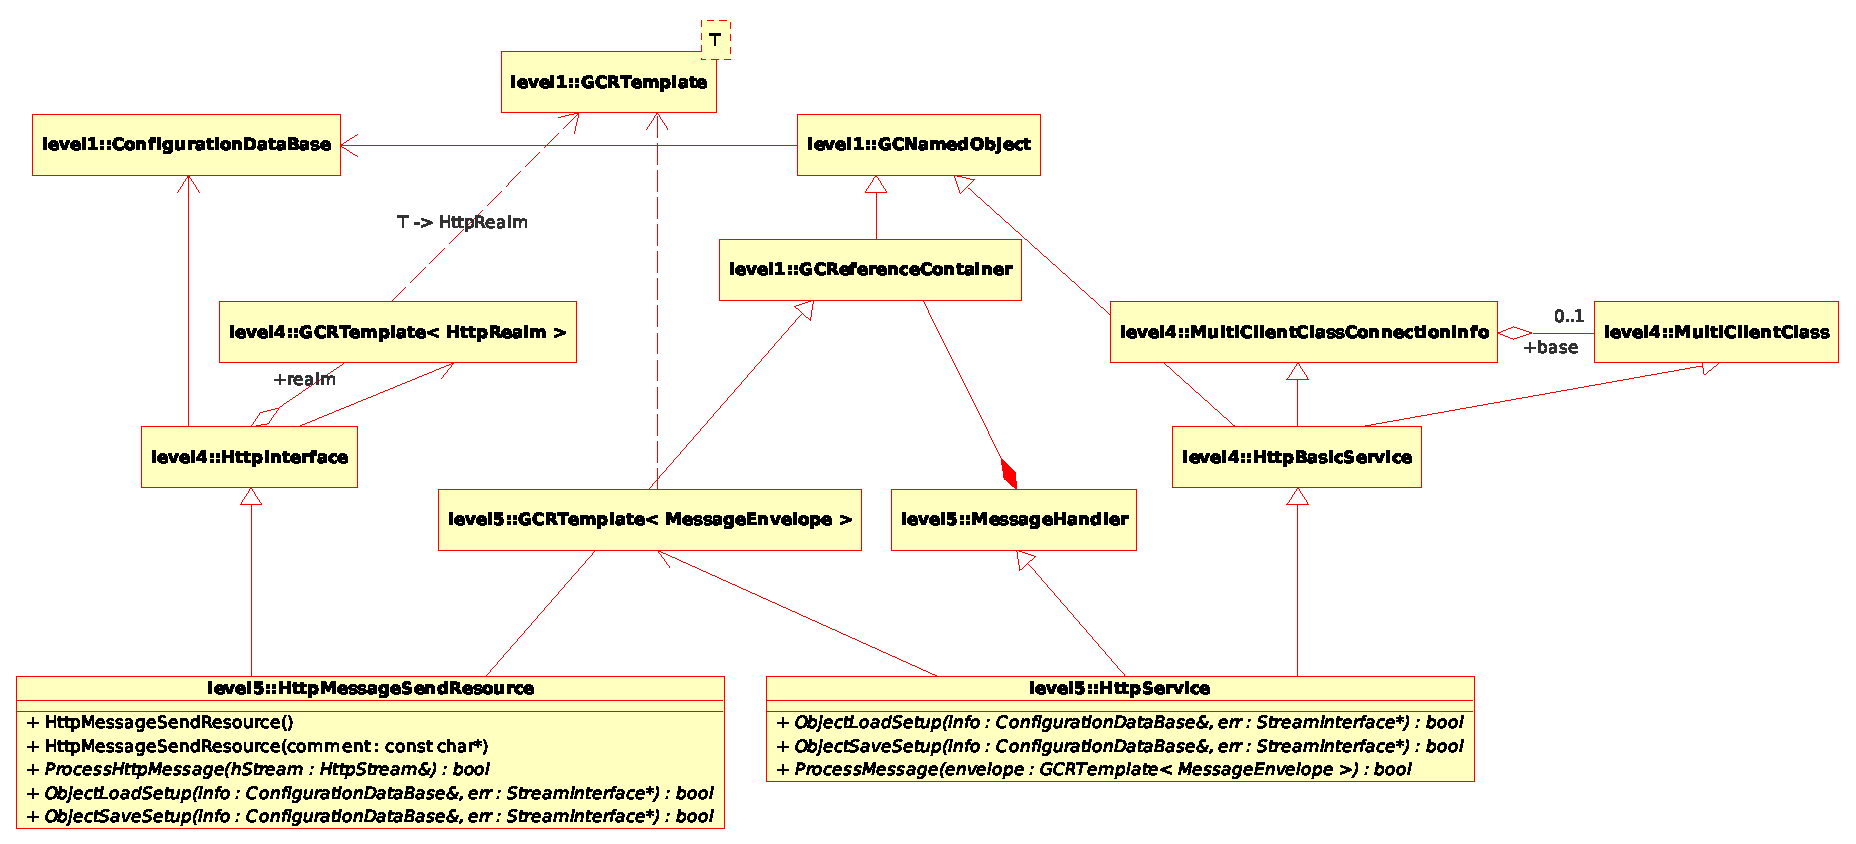
\includegraphics[width=0.88\textwidth]{level5/level5-HTTP.eps} 
  \caption{BaseLib Level 5 HTTP Messages}
  \label{f:level5:MSGHTTP}
 \end{center}
\end{figure}

\subsubsection{HttpMessageSendResource}
\texttt{[HttpMessageSendResource.h, HttpMessageSendResource.cpp]}\\
TODO

\subsubsection{HttpService}
\texttt{[HttpService.h, HttpService.cpp]}\\
TODO



\section{State Machine}
The state machine implemented in this section is an extended one that also deal with errors and system failures, it's similar to the MATLAB$^\copyright$ Stateflow$^\copyright$ behaviour.

Basically a state machine is build up on two sets of elements: firstly a \textbf{set of states} and a \textbf{set of archs} that connect states and identify the happening of an event. When an event is triggered (i.e. by an external event) the state machine is in a state, in this state it will search if there is an associated event's behaviour and if it is the state machine execute the registered actions. If an error occours there is basically an error state to reach.

Actions usually are in form of messages sended between objects, i.e. think about a windows system where each window object can receive and send messages and react on those messages. In fact the state machine is the first entity using the message infrastructure.

\begin{figure}[h!]
 \begin{center}
  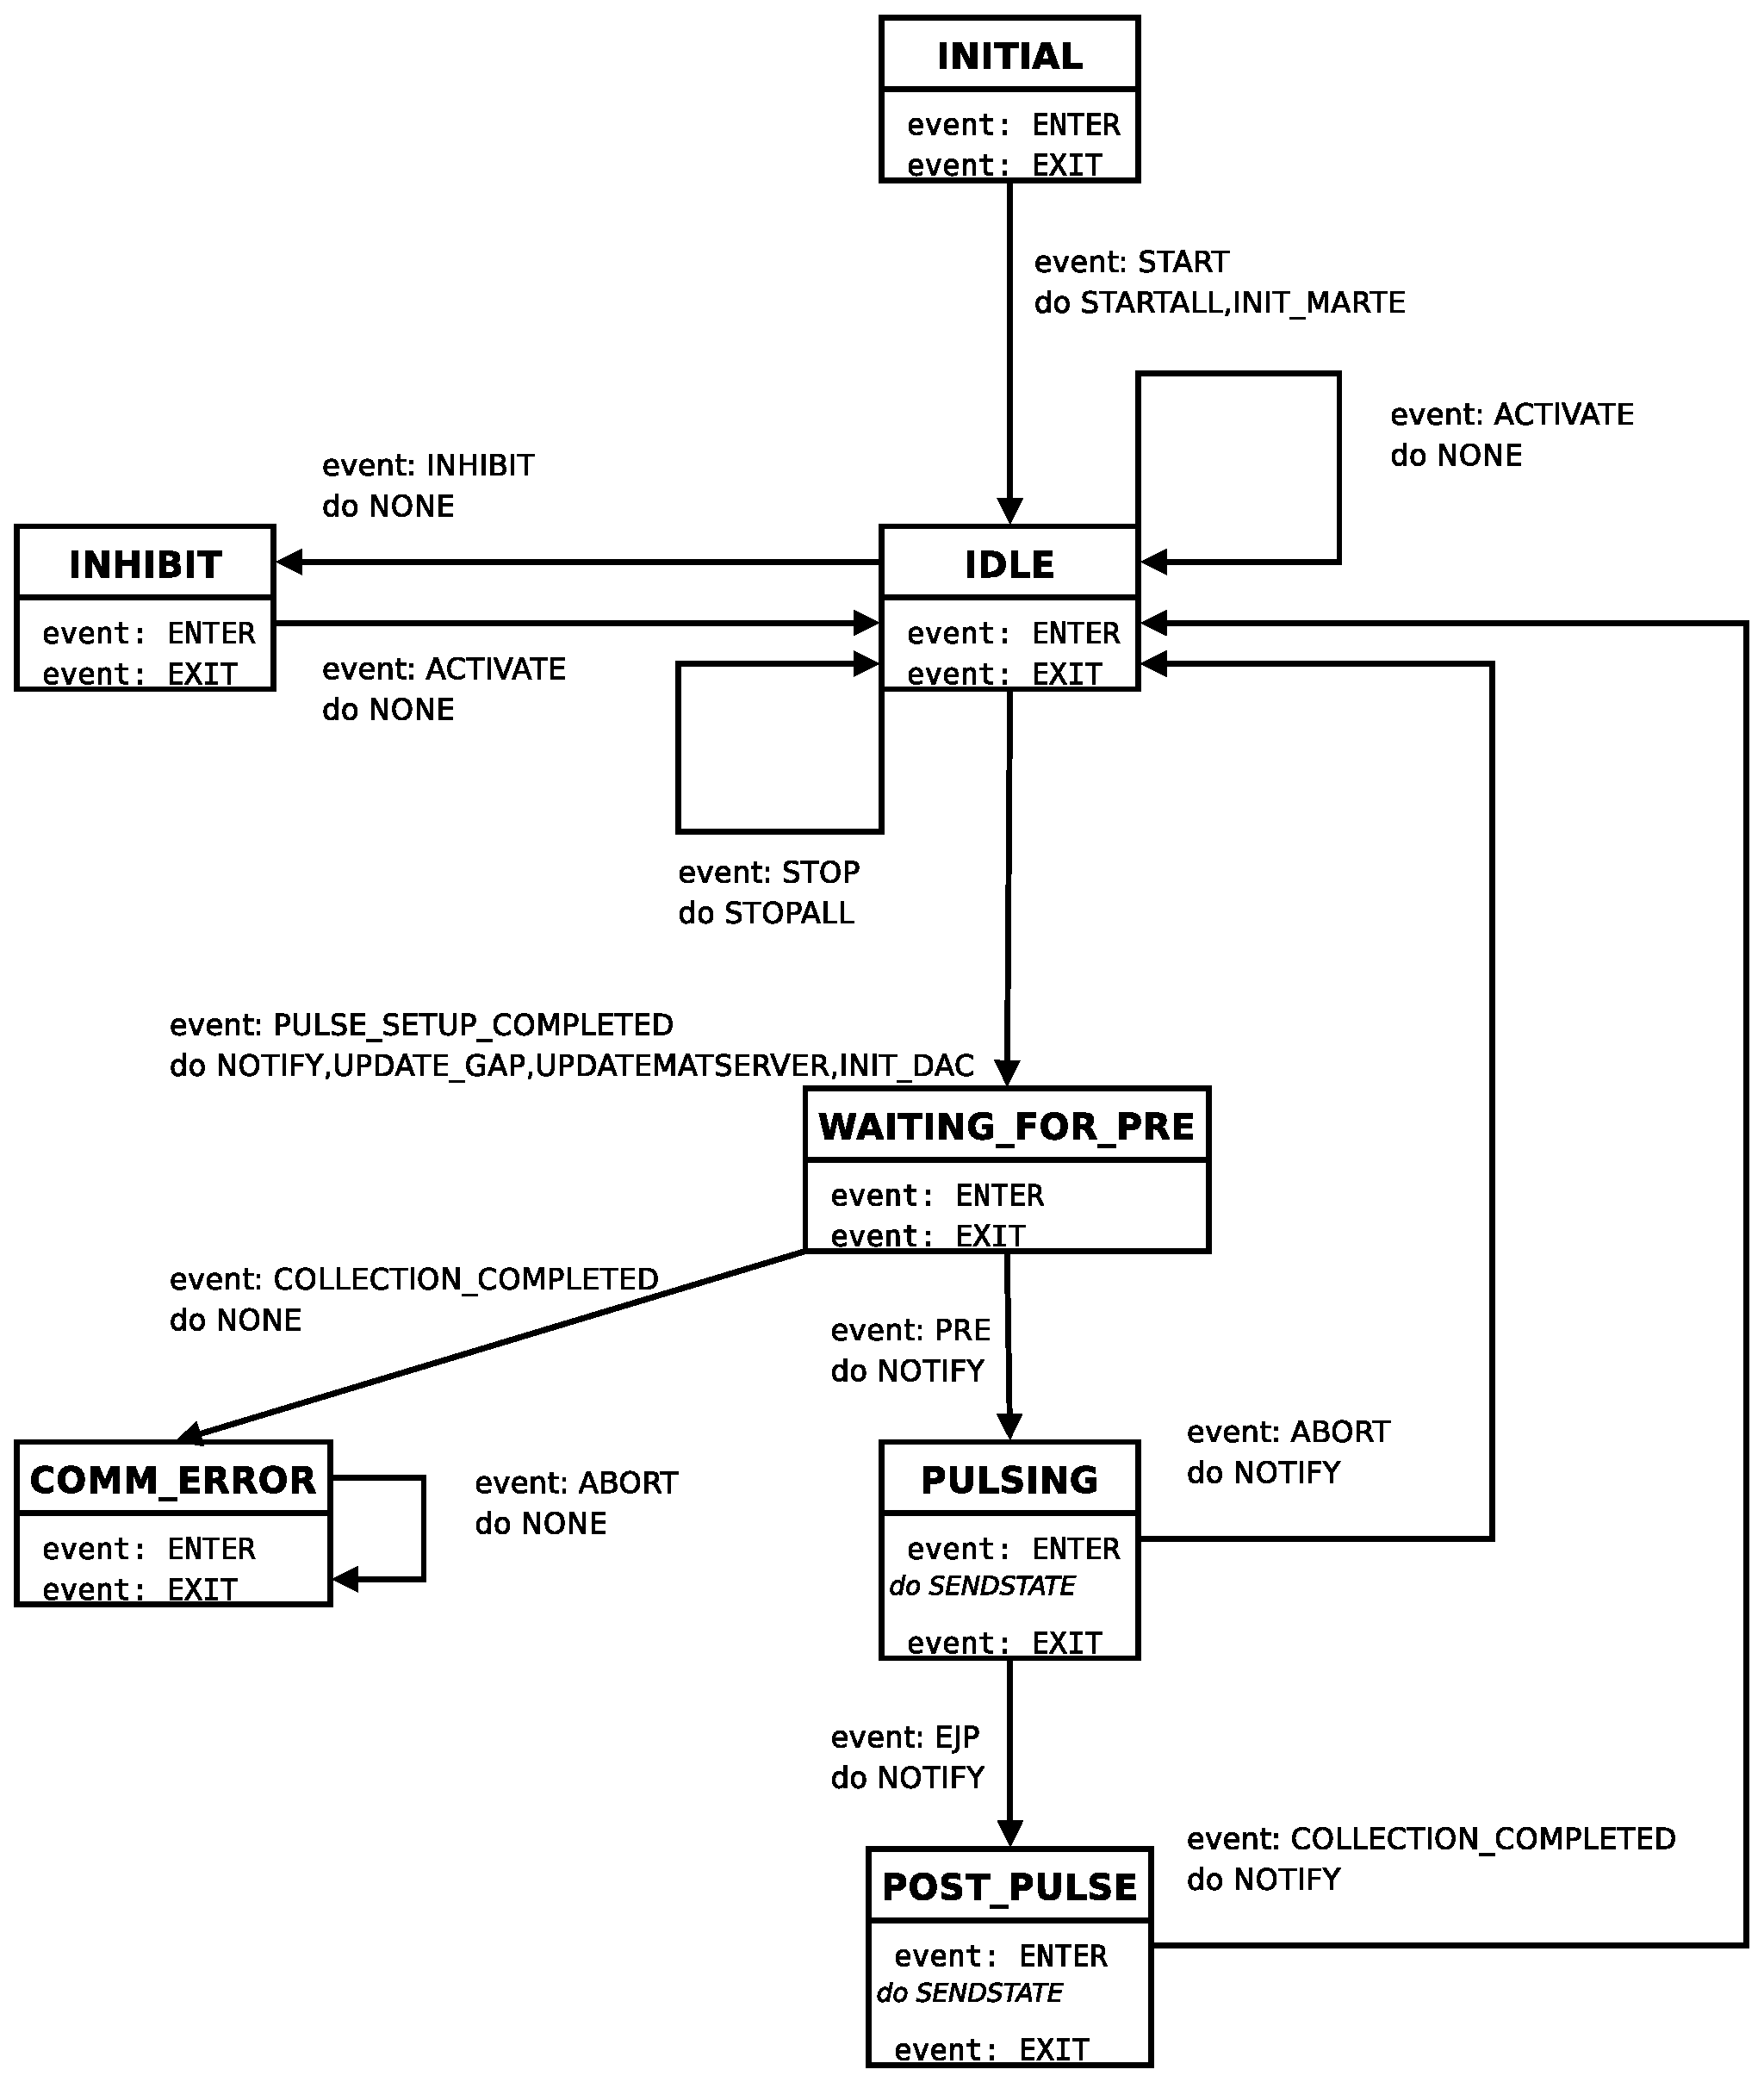
\includegraphics[width=0.55\textwidth]{level5/VS5statemachine.eps}
  \caption{VS5 State Machine example}
  \label{f:level5:VS5SM_example}
 \end{center}
\end{figure}

Figure \ref{f:level5:VS5SM_example} represent an example of the state machine required in the Vertical Stabilization control algorithm. In the following comes an excerpt of the configuration file that generate this state machine. There is no tool right now for the autogeneration of the configuration file from the design (that is actually not fully sketched: default actions, error and fault conditions are not visible).

\begin{lstlisting}[
extendedchars=true,%
basicstyle=\fontfamily{pcr}\fontseries{m}\selectfont\footnotesize, %
stepnumber=1,%
numberstyle=\tiny,%
keywordstyle=\footnotesize\tt ,%
language=bash]
+StateMachine = {
    Class = StateMachine
    VerboseLevel = 10
    +INITIAL = {
        Class = StateMachineState
        StateCode = 0x0
        +START = {
            Class = StateMachineEvent
            NextState = IDLE
            Value = START
            +STARTALL = {
                Class = MessageDeliveryRequest
                Sender = StateMachine
                Destinations = "HTTPSERVER CODAS MARTe"
                MsecTimeOut = 1000
                Flags = NoReply
                Message = {
                    Class = Message
                    Content = START
                }
            }
            +INIT_MARTe = {
...
            }
        }
    }
    +IDLE = { ...
    }
    +WAITING_FOR_PRE = { ...
    }
    +PULSING = { ...
    }
    +POST_PULSE = { ...
    }
    +INHIBIT = { ...
    }
    +COMM_ERROR = { ...
    }
}
\end{lstlisting}

In this example we saw how the configuration file works for a state machine: it really relies on \texttt{GCReferenceContainer} syntax. For each state you can register an action on entry and on exit and a default action. Each arch has a set of actions associated with it. The state machine react to events acting as preconfigured dependent on the current state.

\begin{figure}[h!]
 \begin{center}
  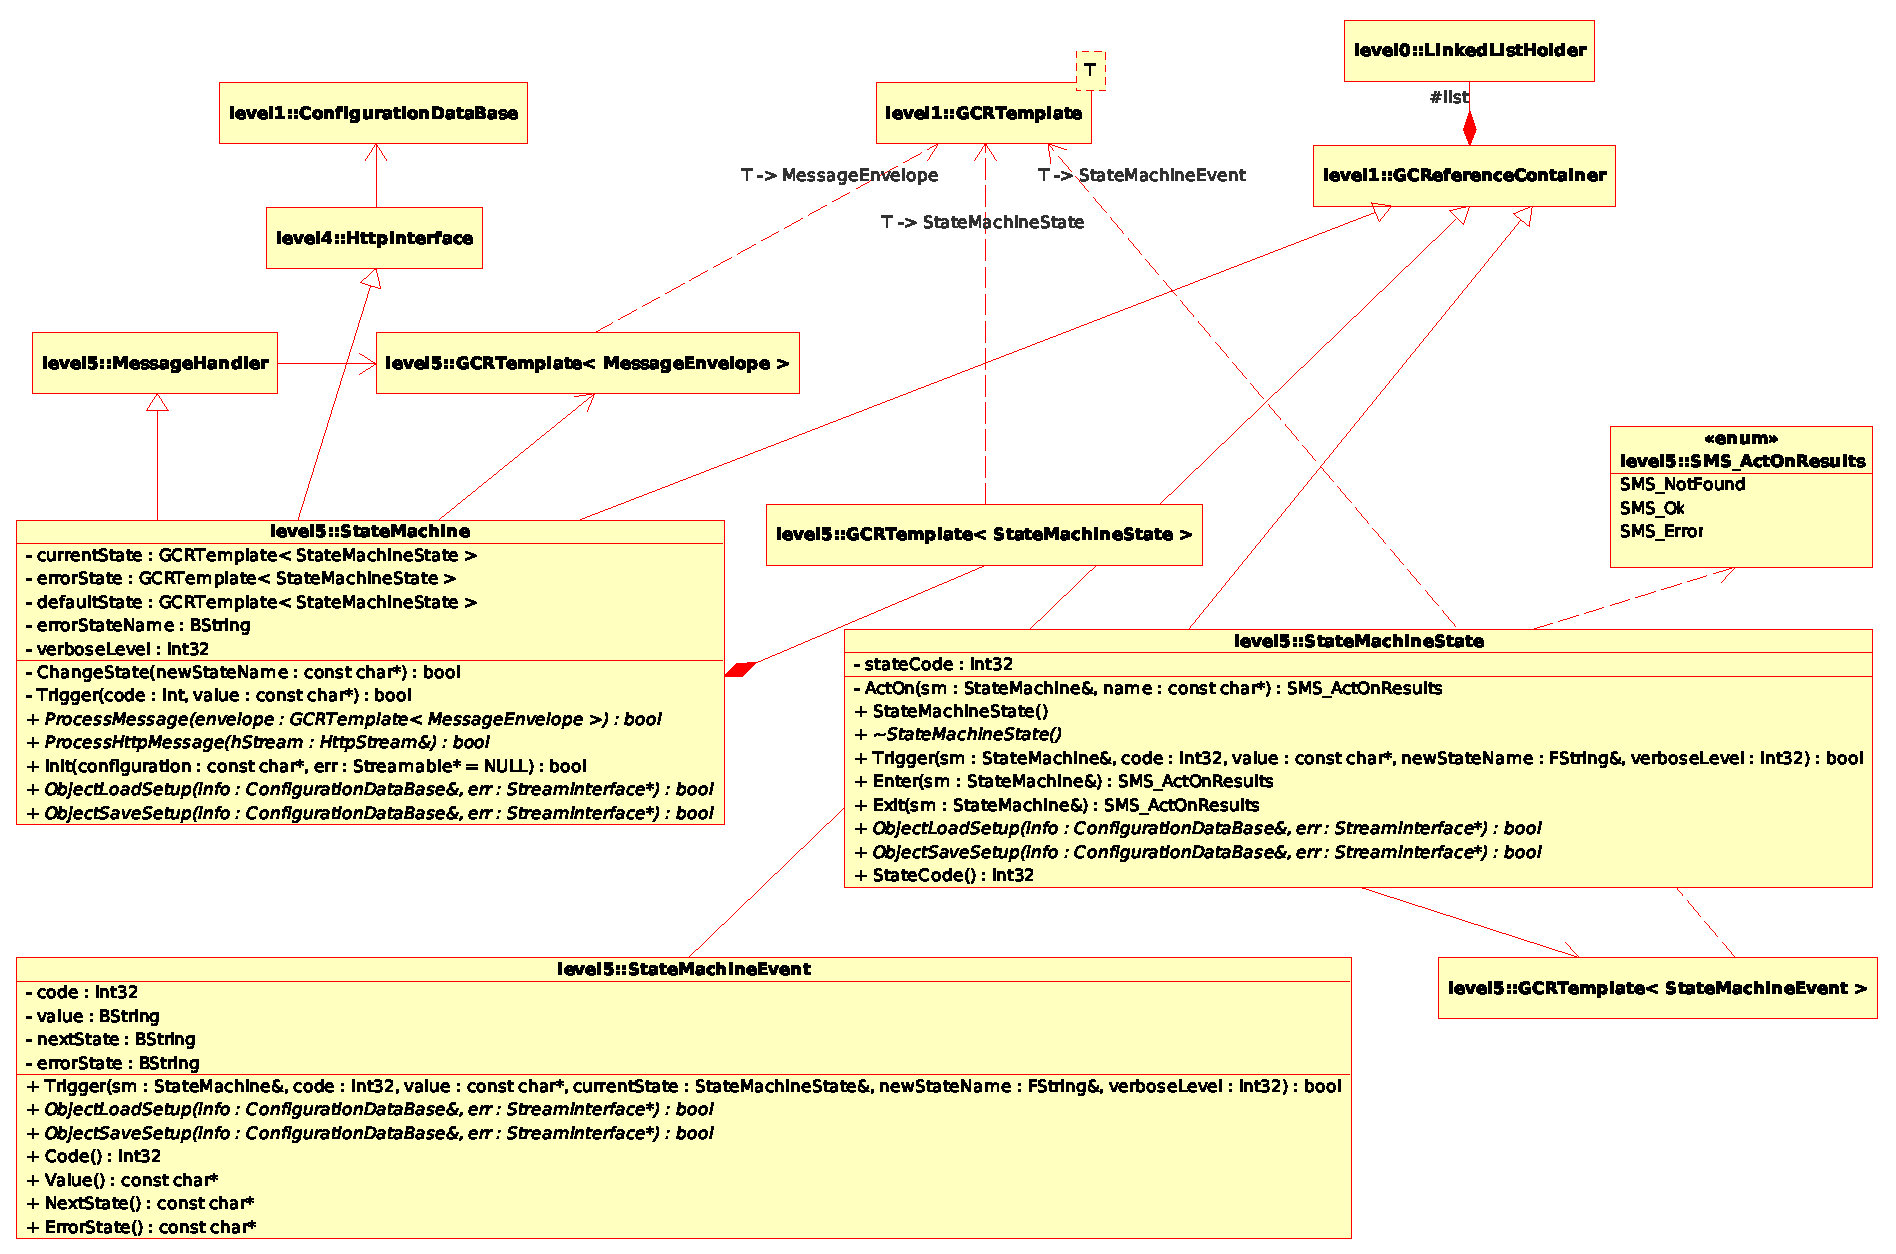
\includegraphics[width=\textwidth]{level5/level5-StateMachine.eps}
  \caption{BaseLib Level 5 State Machine}
  \label{f:level5:SM}
 \end{center}
\end{figure}

Class involved in this section are depicted in the UML schema of Figure \ref{f:level5:SM} and are listed below:
\begin{itemize}
 \item StateMachineState
 \item StateMachineEvent
 \item StateMachine
\end{itemize}



\subsubsection{State Machine State}
\texttt{[StateMachineState.h, StateMachineState.cpp]}\\
The class \texttt{StateMachineState} represents a state within the state machine; the \texttt{StateMachineState} inherits from \texttt{GCReferenceContainer} and so it is a container of \texttt{StateMachineEvent}s or \texttt{MessageDeliveryRequest}s.

There are only two \texttt{MessageDeliveryRequest}s one named \texttt{``ENTER''} and one \texttt{``EXIT''}; these messages are delivered on entering or exiting the state. \\


The enumeration \texttt{SMS\_ActOnResults} is first introducted as below, and is usually the result of some methods implemented in the \texttt{StateMachineState} class.
\begin{lstlisting}[
extendedchars=true,%
basicstyle=\fontfamily{pcr}\fontseries{m}\selectfont\footnotesize, %
stepnumber=1,%
numberstyle=\tiny,%
keywordstyle=\footnotesize\tt ,%
language=C++]
enum SMS_ActOnResults{
   SMS_NotFound = 0,
   SMS_Ok = 1,
   SMS_Error = -1,
};
\end{lstlisting}

The \texttt{stateCode} class's attribute is a code associated with this state. The first, private method, \texttt{ActOn} perform the activity called \texttt{name} and returns \texttt{SMS\_NotFound} if the action was not found or \texttt{SMS\_Error} in case of errors; the method \texttt{ActOn} searches for a \texttt{name} classes throught the list holded by the \texttt{GCReferenceContainer} superclass, it tries to cast it first to a \texttt{MessageEnvelope} and then to a \texttt{MessageDeliveryRequest}. If it succeeds to cast to \texttt{MessageEnvelope} searchs again for a \texttt{``SENDSTATE''} message; otherwise compares the mesagge string with the \texttt{``SENDSTATE''} string; then send the message, the \texttt{StateMachine} passed by argument is the source object.\\


The constructor sets the \texttt{stateCode} attribute to zero. The destructor does anything usefull. The method \texttt{Trigger} finds this trigger and execute the associated actions returning the new state; the trigger infrastructure deals with \texttt{StateMachineEvent}s. \texttt{Enter} simply calls the method \texttt{ActOn} with \texttt{name} setted to \texttt{``ENTER''}, the method \texttt{Exit} with \texttt{``EXIT''}.\\


The common method \texttt{ObjectLoadSetup} initialises an object from a set of configs, the syntax is the same as \texttt{GCReferenceContainer} one shall also define a code using \texttt{StateCode = nnn}; the main container content should be only of class \texttt{StateMachineEvent}; if an object called \texttt{``ENTER''} is added, of type \texttt{MessageDeliveryRequest} or \texttt{MessageEnvelope} than a message is sent on entry; if an object called \texttt{``EXIT''} is added of type \texttt{MessageDeliveryRequest} or \texttt{MessageEnvelope} than a message is sent on exit; if a \texttt{StateMachineEvent} called \texttt{``DEFAULT''} is encountered while matching the trigger then a match is always automatically found; the object name is taken from the current node name if a \texttt{MessageEnvelope} or \texttt{MessageDeliveryRequest} with the first object contained being a \texttt{Message} called \texttt{``SENDSTATE''} is found than the current state is used as content for that \texttt{Message}. In this case the \texttt{MessageEnvelope} and \texttt{MessageDeliveryRequest} are duplicated, note that the current state not the final state are sent.

\texttt{ObjectLoadSetup} saves an object to a set of configs, the syntax is the same as \texttt{GCReferenceContainer}; the container content should be only of class \texttt{StateMachineState}. The object name is taken from the current node name.

\begin{lstlisting}[
extendedchars=true,%
basicstyle=\fontfamily{pcr}\fontseries{m}\selectfont\footnotesize, %
stepnumber=1,%
numberstyle=\tiny,%
keywordstyle=\footnotesize\tt ,%
language=C++]
private:
   int32 stateCode;

   SMS_ActOnResults ActOn(StateMachine& sm,const char* name);
public:
   StateMachineState();
   virtual ~StateMachineState();

   bool Trigger(StateMachine& sm,int32 code,const char* value,FString& newStateName,int32 verboseLevel);
   inline SMS_ActOnResults Enter(StateMachine& sm);
   inline SMS_ActOnResults Exit(StateMachine& sm);

   virtual bool ObjectLoadSetup(ConfigurationDataBase& info,StreamInterface* err);
   virtual bool ObjectSaveSetup(ConfigurationDataBase& info,StreamInterface* err);
   inline int32 StateCode();
\end{lstlisting}



\subsubsection{State Machine}
\texttt{[StateMachine.h, StateMachine.cpp]}\\
The class \texttt{StateMachine} is a generic state machine that reacts to messages and acts by sending messages. The code is organized as a container of \texttt{StateMachineState} and a \texttt{MessageHandler}: when it receives a message it matches it to the \texttt{StateMachineEvent} contained in the \texttt{currentState}.

If code matches or if (code equal zero) content matches than it sends all the messages contained in \texttt{StateMachineEvent}. A reply to the original message is sent with the parameters (State\_code,"State\_label") if the original message required manual reply ErrorState is the state the machine reaches if the specified state cannot be found. By default its value is ERROR but if ERROR does not exist then the state will not change. See StateMachineState for the ENTER EXIT action objects and for the Events. If any of the ENTER or EXIT actions fail the state machine will reach ErrorState DEFAULT is a state whose Events and ENTER/EXIT actions are appended to those of the current state if the next state is specified as \texttt{``SAMESTATE''} this means that not change of state will occurr; if a \texttt{MessageEnvelope} or \texttt{MessageDeliveryRequest} with the first object contained being a \texttt{Message}  called \texttt{``SENDSTATE''} is found than the current state is used as content for that \texttt{Message}. In this case the \texttt{MessageEnvelope} and \texttt{MessageDeliveryRequest} are duplicated. Note that the current state not the final state are sent 

class StateMachine: public GCReferenceContainer, public MessageHandler, public HttpInterface



The first three attributes are all of type \texttt{GCRTemplate<StateMachineState>} the first one is a refrence to the currently active state: initialised with the first state; refrence to the default error state: last state or the one called \texttt{``ERROR''} and the last is another reference to a state called \texttt{``DEFAULT''}. \texttt{``ENTER''} and \texttt{``EXIT''} messages are executed before and after the state specific ones at every state change.
The attribute \texttt{errorStateName} is the name of the error state, by default \texttt{``ERROR''}; if \texttt{verboseLevel} is zero means no diagnostics, $1$ shows all the state changes.
\begin{lstlisting}[
extendedchars=true,%
basicstyle=\fontfamily{pcr}\fontseries{m}\selectfont\footnotesize, %
stepnumber=1,%
numberstyle=\tiny,%
keywordstyle=\footnotesize\tt ,%
language=C++]
   GCRTemplate<StateMachineState> currentState;
   GCRTemplate<StateMachineState> errorState;
   GCRTemplate<StateMachineState> defaultState;
   BString errorStateName;
   int32 verboseLevel;
\end{lstlisting}

The method \texttt{ChangeState} implement a change of state if \texttt{newStateName == SAMESTATE} will not change state returns \texttt{true} if the state has changed.

\texttt{Trigger} processes the \texttt{code} or \texttt{value} arguments to determine the next state.

The \texttt{StateMachine} is basically a \texttt{MessageHandler} so it should implement the \texttt{MessageHandlerInterface} providing \texttt{ProcessMessage} or \texttt{ProcessMessage2} for incoming message handling. \texttt{ProcessHttpMessage} is the main entry point for \texttt{HttpInterface}.

\texttt{Init} creates a menu tree creating a stream first then a CDB and then using ObjectLoadSetup.

The usual \texttt{ObjectLoadSetup} and \texttt{ObjectSaveSetup} come; for both the syntax is the same as \texttt{GCReferenceContainer}, the container content should be only of class StateMachinState optional parameter is ErrorStateName which allows selecting the ErrorState; if NextState is SAMESTATE no change will occur VerboseLevel {integer} if set >0 will cause diagnostic messages to appear >=1 shows status changes >=2 shows actions performed >=10 shows message processing details; the object name is taken from the current node name.

\begin{lstlisting}[
extendedchars=true,%
basicstyle=\fontfamily{pcr}\fontseries{m}\selectfont\footnotesize, %
stepnumber=1,%
numberstyle=\tiny,%
keywordstyle=\footnotesize\tt ,%
language=C++]
   bool ChangeState(const char* newStateName);
   bool Trigger(int code,const char* value);

public:
   virtual bool ProcessMessage(GCRTemplate<MessageEnvelope> envelope);
   virtual bool ProcessHttpMessage(HttpStream& hStream);

   bool Init(const char* configuration,Streamable* err=NULL);

   virtual bool ObjectLoadSetup(ConfigurationDataBase& info,StreamInterface* err);
   virtual bool ObjectSaveSetup(ConfigurationDataBase& info,StreamInterface* err);
\end{lstlisting}



\subsubsection{StateMachineEvent}
\texttt{[StateMachineEvent.h, StateMachineEvent.cpp]}\\
The class \texttt{StateMachineEvent} is an event contained(referred to) within a state. This is a container of \texttt{MessageDeliveryRequest} it also can contains a set of \texttt{StateMachineState}.
The \texttt{StateMachineEvent} class is also a \texttt{GCReferenceContainer}.

The first attribute \texttt{code} is a code associated with this event, zero means use the \texttt{value} attribute; such attribute is a string value associated with this event. When this event occurs the next state has name \texttt{nextState} and if the action fails we go to \texttt{errorState}.
\begin{lstlisting}[
extendedchars=true,%
basicstyle=\fontfamily{pcr}\fontseries{m}\selectfont\footnotesize, %
stepnumber=1,%
numberstyle=\tiny,%
keywordstyle=\footnotesize\tt ,%
language=C++]
   int32 code;
   BString value;
   BString nextState;
   BString errorState;
\end{lstlisting}

The method \texttt{Trigger} performs the action associate with a trigger.

\texttt{ObjectLoadSetup} initialises an object from a set of configs; the syntax is the same as GCReferenceContainer; the container content should be only of class \texttt{MessageEnvelope} or \texttt{MessageDeliveryRequest} important parameters are:

\begin{table}[!h]
  \begin{tabular}{ll}
\texttt{Code} & (an integer) or \\
\texttt{UserCode} &(an integer) \\
\texttt{Value} & (a string) that identify the trigger \\
\texttt{NextState} & (a string) is the next state and \\
\texttt{ErrorState} & (a string) is the next state on error \\
  \end{tabular}
\end{table}

The object name is taken from the current node name. If the object is called \texttt{``DEFAULT''} than it matches any message code, if a \texttt{MessageEnvelope} or \texttt{MessageDeliveryRequest} called \texttt{
``SENDSTATE''} is founded than the current state is added as content. In this case the \texttt{MessageEnvelope} and \texttt{MessageDeliveryRequest} are duplicated. Note that the current state not the final state are sent. \texttt{ObjectSaveSetup} saves an object to a set of configs.\\


Then follows a set of getter methods that returns the attributes content.
\begin{lstlisting}[
extendedchars=true,%
basicstyle=\fontfamily{pcr}\fontseries{m}\selectfont\footnotesize, %
stepnumber=1,%
numberstyle=\tiny,%
keywordstyle=\footnotesize\tt ,%
language=C++]
public:
   bool Trigger(StateMachine& sm,int32 code,const char* value,StateMachineState& currentState,FString& newStateName,int32 verboseLevel);

   virtual bool ObjectLoadSetup(ConfigurationDataBase& info,StreamInterface* err);
   virtual bool ObjectSaveSetup(ConfigurationDataBase& info,StreamInterface* err);

   int32 Code();
   const char* Value();
   const char* NextState();
   const char* ErrorState();
\end{lstlisting}



\section{Signals}

Class involved in this section are depicted in the UML schema of Figure \ref{f:level5:Signal} and are listed below:
\begin{itemize}
 \item SignalInterface
 \item Signal
\end{itemize}

\begin{figure}[h!]
 \begin{center}
  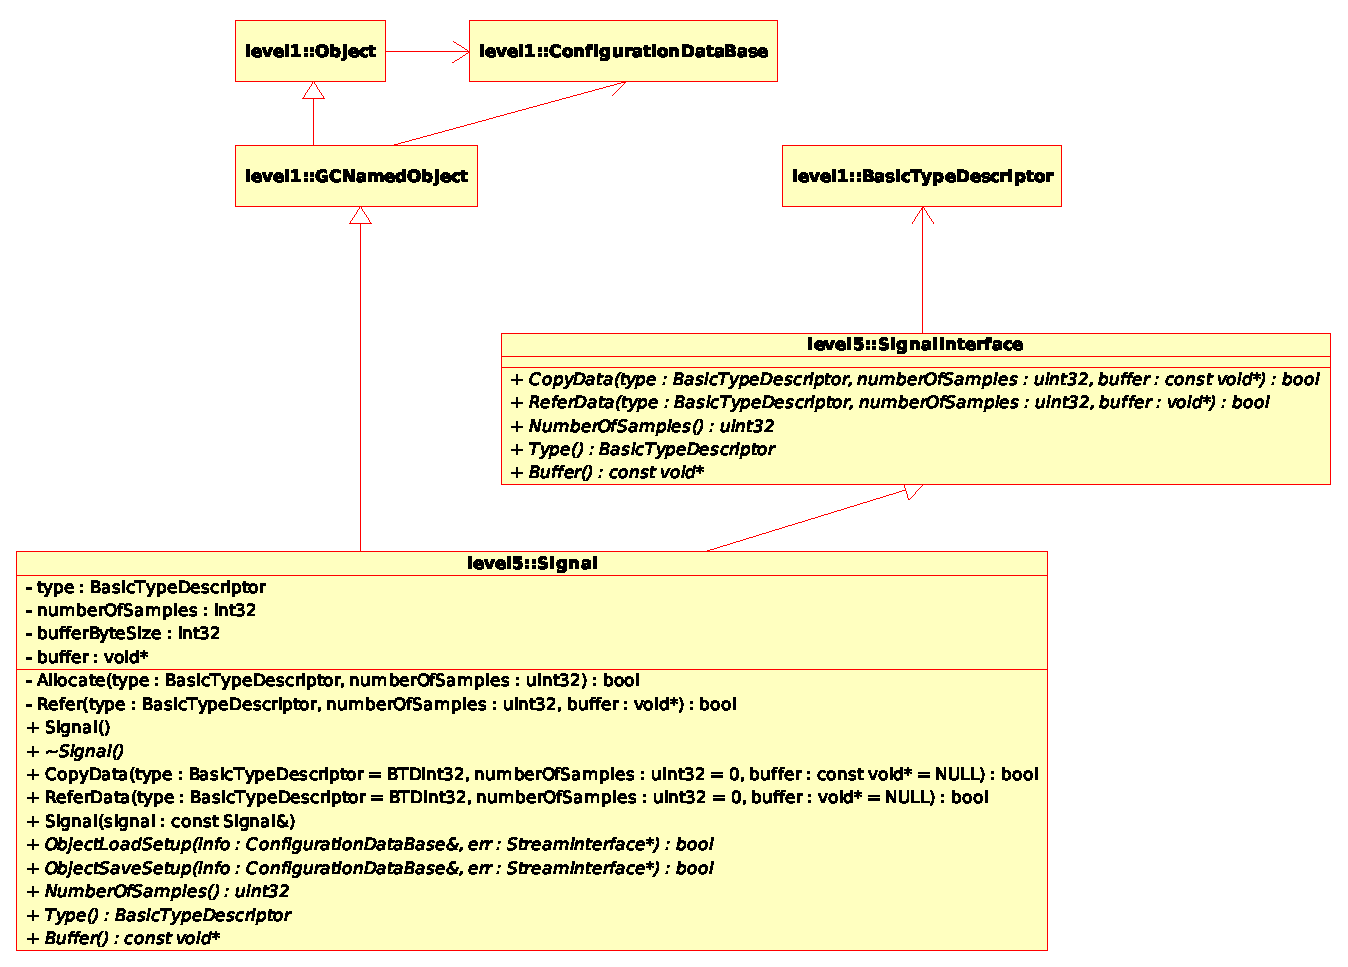
\includegraphics[width=0.77\textwidth]{level5/level5-Signal.eps}
  \caption{BaseLib Level 5 Signal interface classes}
  \label{f:level5:Signal}
 \end{center}
\end{figure}



\subsubsection{SingalInterface}
\texttt{[SignalInterface.h]}\\

\subsubsection{Signal}
\texttt{[Signal.h, Signal.cpp]}\\



\section{Dynamic Data Buffer}
The Dynamic Data Buffer (DDB) is a memory data bus. Different entity could connect to such bus and as happens in an hardware bus each entity could write and read from other entity connected to the bus, the DDB infrastructure let such entity simply communicate providing a sort of shared memory buffers. This is not implemented like a shared memory in an Operating System way. It is not the same concept of the Memory Data Bus developed in the QNX$^\copyright$ microkernel architecture. Refer to the following Figure \ref{f:level5:DDB:VS5} to visualize what a DDB is an looks like.

\begin{figure}[h!]
 \begin{center}
  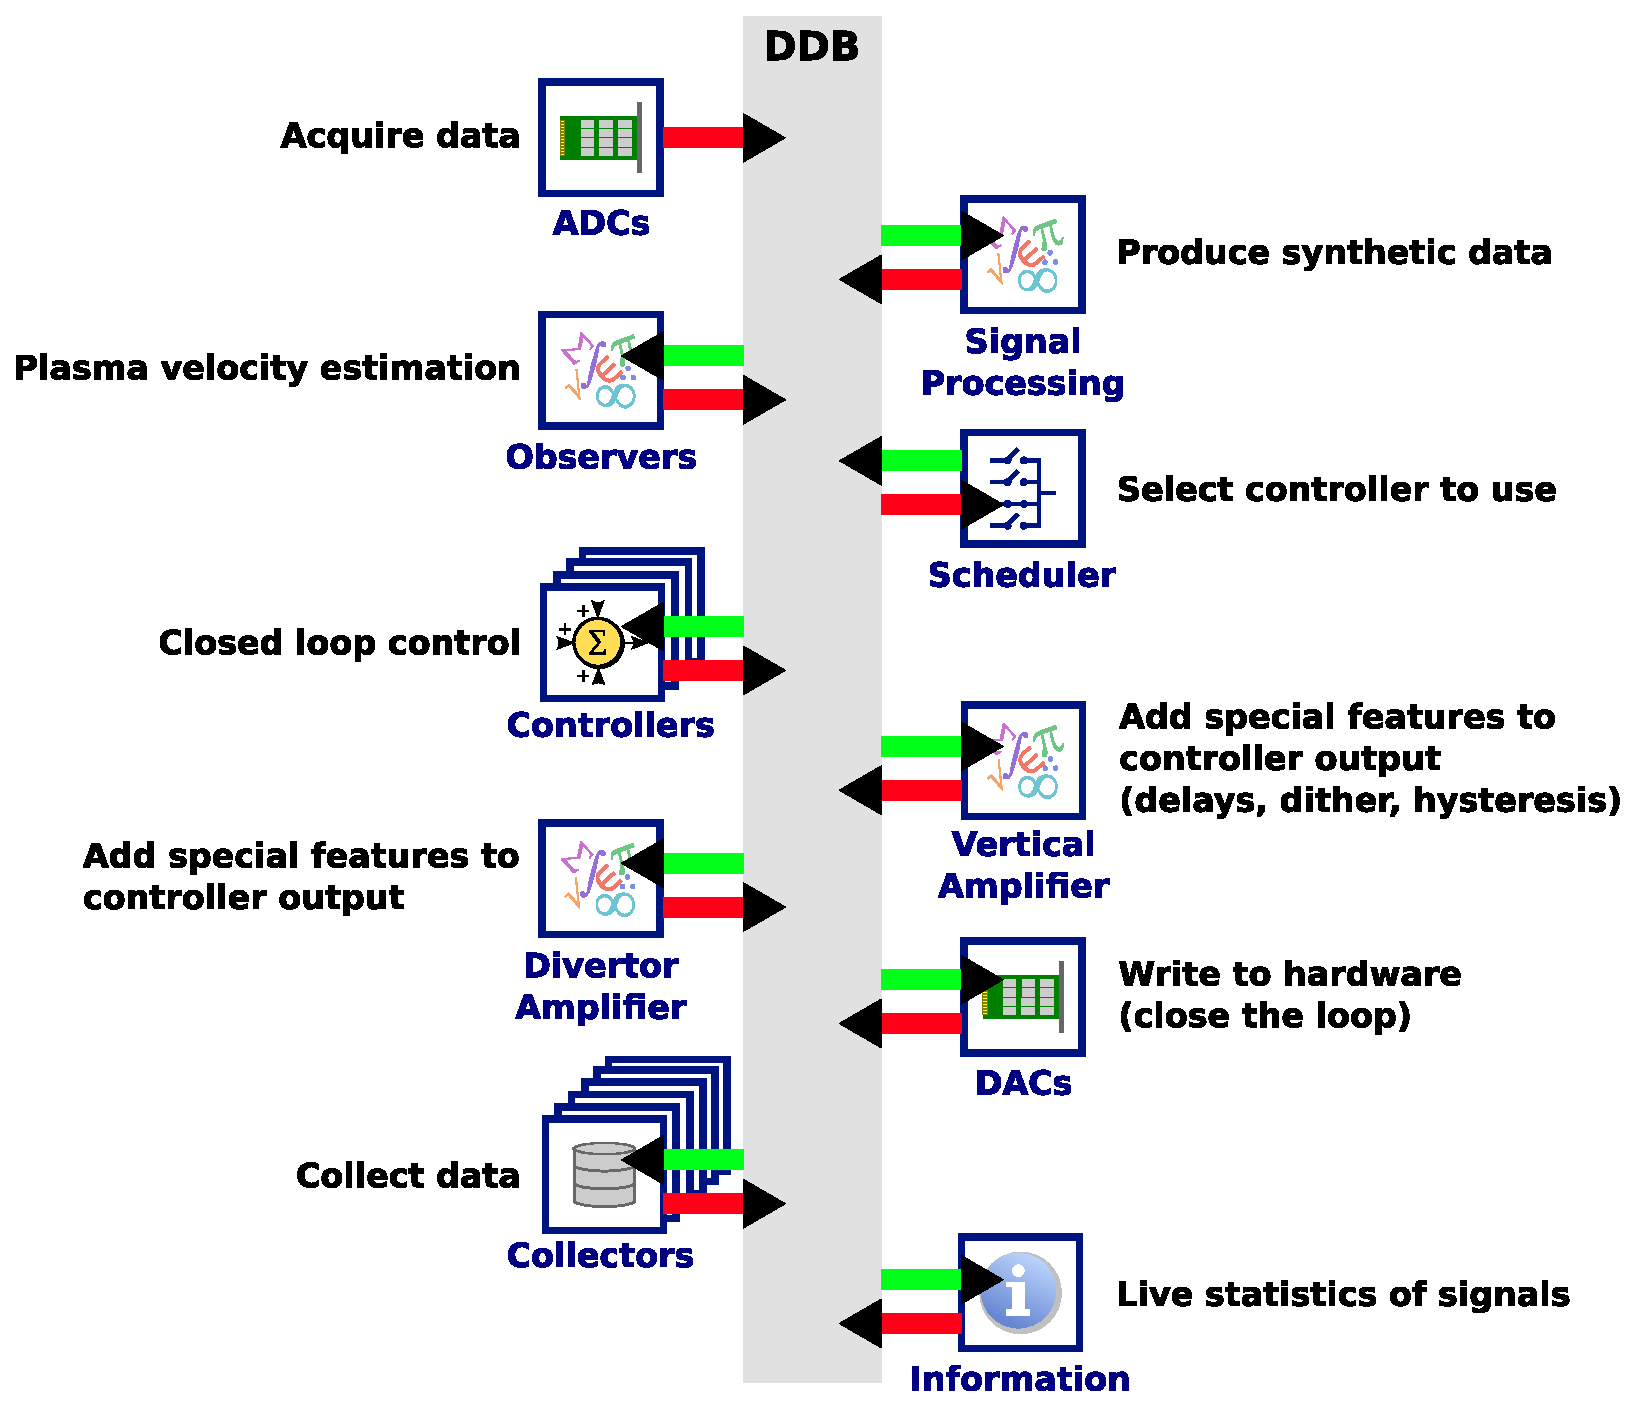
\includegraphics[width=0.5\textwidth]{images/VS5-GAMs2.eps}
  \caption{BaseLib Level 5 DDB setup for the Vertical Stabilization ver 5.0}
  \label{f:level5:DDB:VS5}
 \end{center}
\end{figure}

Each entity connected to the described memory bus is called Generic Application Module (GAM), in Figure \ref{f:level5:DDB:VS5} there are different GAMs: ADC, Signal Processing, Observer, Scheduler, Controller, Vertical Amplifier, Divertor Amplifier, DAC, Collector, Information; each GAM can be associated with a physical piece of hardware, like an ADC, or not.
%ANDRE articolo --- start ---
Data is transferred between GAMs using the Dynamic Data Buffer. The first role of such tool is to ensure coherency across the system, verifying if all the signals requested by each of the GAMs is produced by one module and in case of any inconsistency issue an error. Although it is not the default behavior, a GAM may write over a signal already produced by another module. This process, named patching, must be explicitly requested otherwise it is assumed as an error.
%ANDRE articolo --- end ---
Each GAMs can produce and/or consume data and so will be an output, input or IO GAM. Figure \ref{f:level5:DDB:VS5detail} illustrate a path of data between e producer GAM and an IO GAM. \\

\begin{figure}[h!]
 \begin{center}
  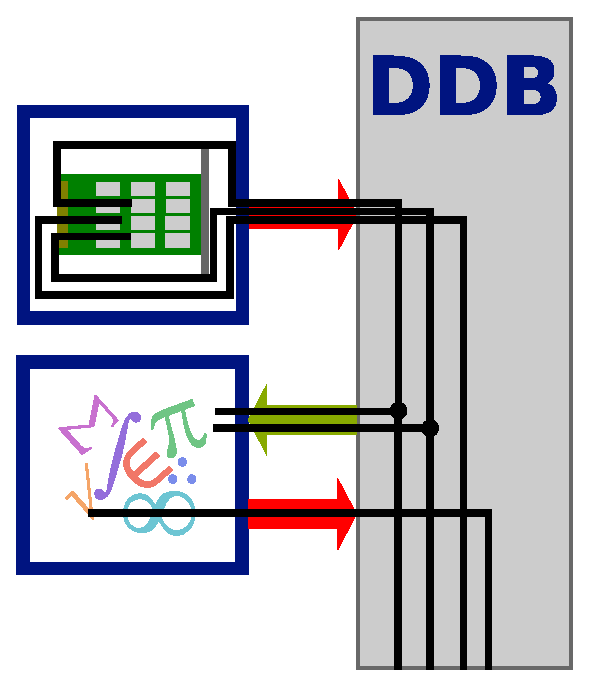
\includegraphics[width=0.33\textwidth]{images/DDBDetail.eps}
  \caption{BaseLib Level 5 DDB setup for the Vertical Stabilization ver 5.0 (detail view)}
  \label{f:level5:DDB:VS5detail}
 \end{center}
\end{figure}

The DDB is a really powerfull tool but the internal architecture is far away to be simple and use many underlying data structures that can be integrated in the class itself. \\


The Dynamic Data Buffer is basically a buffer, i.e. a piece of memory area, this memory is divided in a way that each signal can be written and readed in a smart way. If we think about a control system, this system is usually represented by blocks (like in Matlab$^\copyright$ Simulink$^\copyright$) and each block has many connection points that are named \textit{interface}s. Each interface loop togheter many \textit{signal}s. A Generic Application Module (GAM) is a block. \\


A GAM can be an IO device as well as an algorithm, anyway a GAM is a set of interfaces (class \texttt{DDBInterface}) and an interface is a set of signals (or signal descriptors, class \texttt{DDBSignalDescriptor}). Each signal is distinguished by a name, a basic type and a set of storing properties, thanks to the DDBInterface to each signal a memory buffer can be associated. In Figure \ref{f:level5:DDB:DDBInterface_logic} the UML/logic diagram of the interfaces is depicted, in Figure \ref{f:level5:DDB:GAM_logic} the GAM internals are depicted.

\begin{figure}[h!]
 \begin{center}
  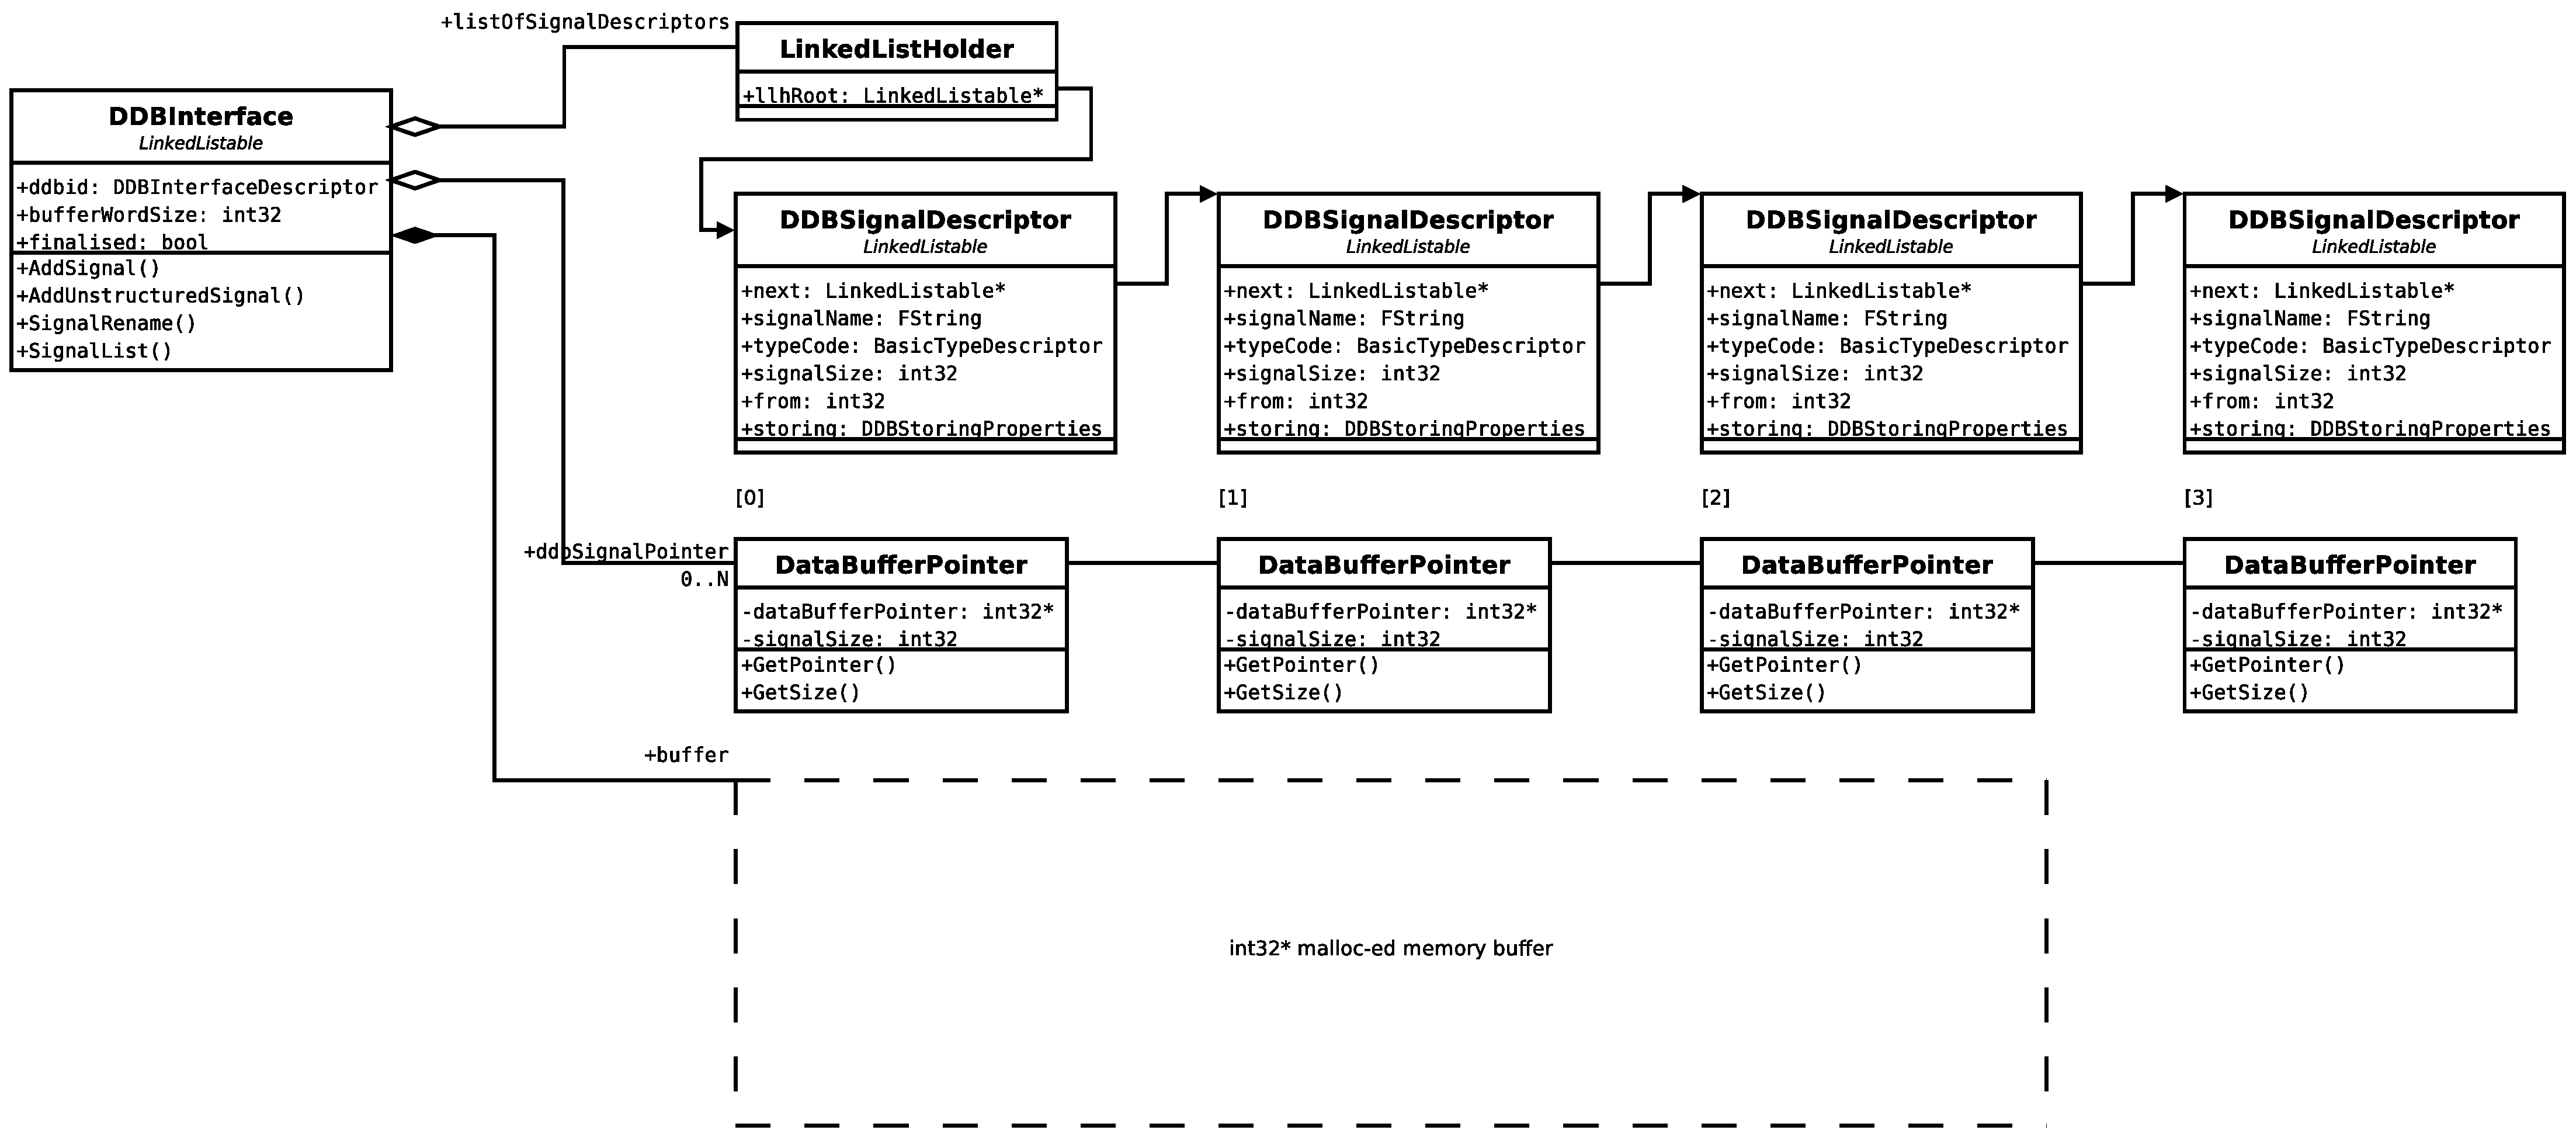
\includegraphics[width=\textwidth]{level5/DDBInterface_logic.eps}
  \caption{BaseLib Level 5 DDB, DDBInterface UML/logic scheme}
  \label{f:level5:DDB:DDBInterface_logic}
 \end{center}
\end{figure}
\begin{figure}[h!]
 \begin{center}
  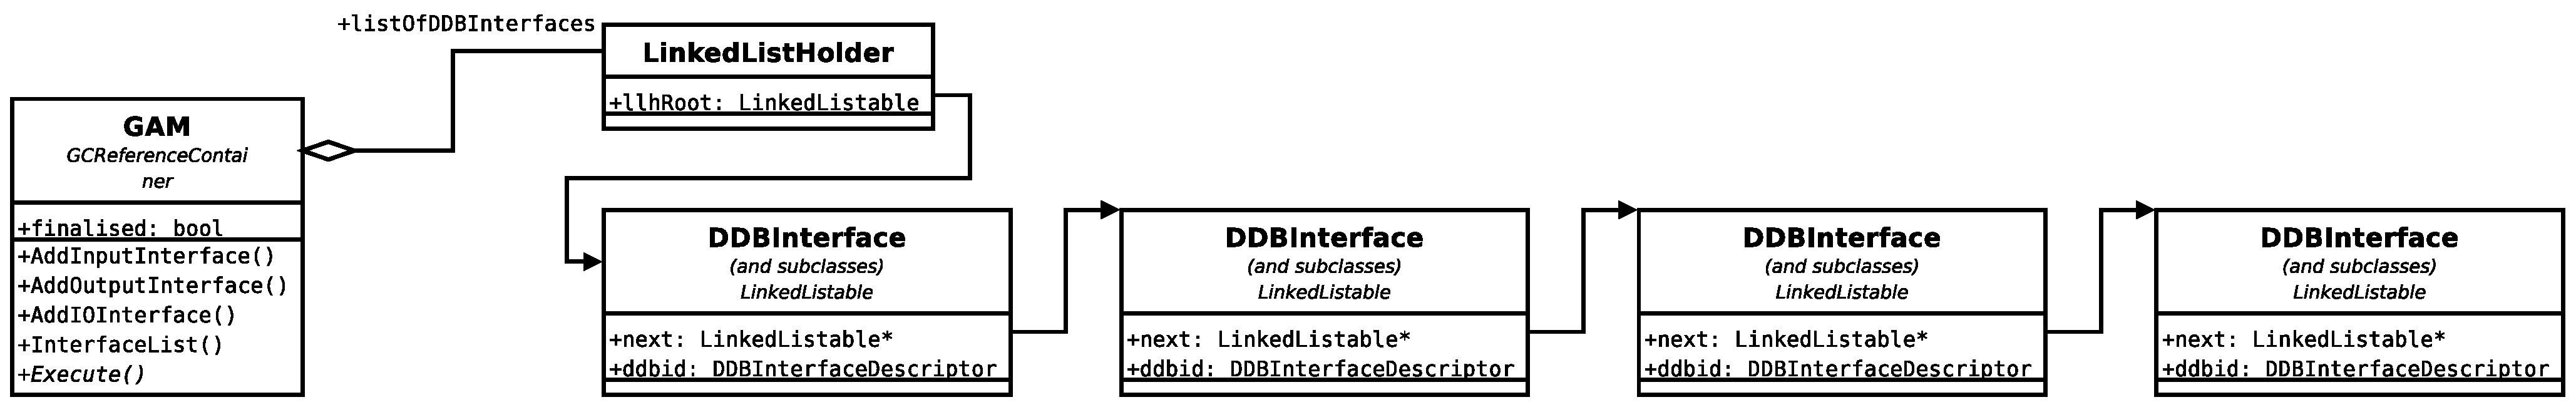
\includegraphics[width=\textwidth]{level5/GAM_logic.eps}
  \caption{BaseLib Level 5 DDB, GAM UML/logic scheme}
  \label{f:level5:DDB:GAM_logic}
 \end{center}
\end{figure}


A DDB take as inputs some GAMs, then analizes its connection and creates the buffers assigning to each signal a predeterminated space (that an interface has asked for), when the DDB is created the DDB can be used. GAMs are tightly bounded with the DDB, infact they were designed togheter.
Steps to make a DDB from a set of GAMs, i.e. connecting GAMs togheter, are:
\begin{enumerate}
 \item create the \texttt{GAM}s (i.e. via the CDB)
 \item for each \texttt{DDBInterface} in each \texttt{GAM} call \texttt{DDB::AddInterface}
 \item a \texttt{DDBItem} will be created for each \texttt{DDBSignalDescriptor}
 \item then call \texttt{DDB::CheckAndAllocate}, this method compute each signal offset in the DDB buffer and check properties of different memory areas
 \item for each GAM call \texttt{DDB::CreateLink}, every \texttt{DataBufferPointer} (in each \texttt{DDBInterface}) will be filled with the correct pointers.
 \item the DDB is ready to be used.
\end{enumerate}

To summarize the insights of the DDB we can make the following reasonment: each GAM represent a block in a control scheme, in each block there are some or any signals as input and some or any signals as output, some input signals can be control signal as well as the output ones. Each signal is grouped togheter to any other following some properties rule and others, i.e. each group of signal has a logical meaning. Each interface of a block can be connected to one or other interfaces of other blocks, and then the signals can flow between interfaces. \\

When the DDB is finalised the basic piece of information that flows between blocks (GAMs) is the signal data. Basically what the DDB does is to create a map between each signal i.e. it creates a list of all signals involved at runtime and gives to each producer/consumer the same address of that signal allocating once the space for it. So first the users work with GAMs that are block centric and uses many interface that contains signals then when it want that those blocks communicate creates a DDB that is signal centric and let blocks transfer the data throught it. \\


Everytime a new GAMs is added to the DDB each signal not just added to the DDB is added as a \texttt{DDBItem}, on \texttt{DDB::CheckAndAllocate} every connection is checked about rights and the summ of the total memory space to allocate is done.

\begin{figure}[h!]
 \begin{center}
  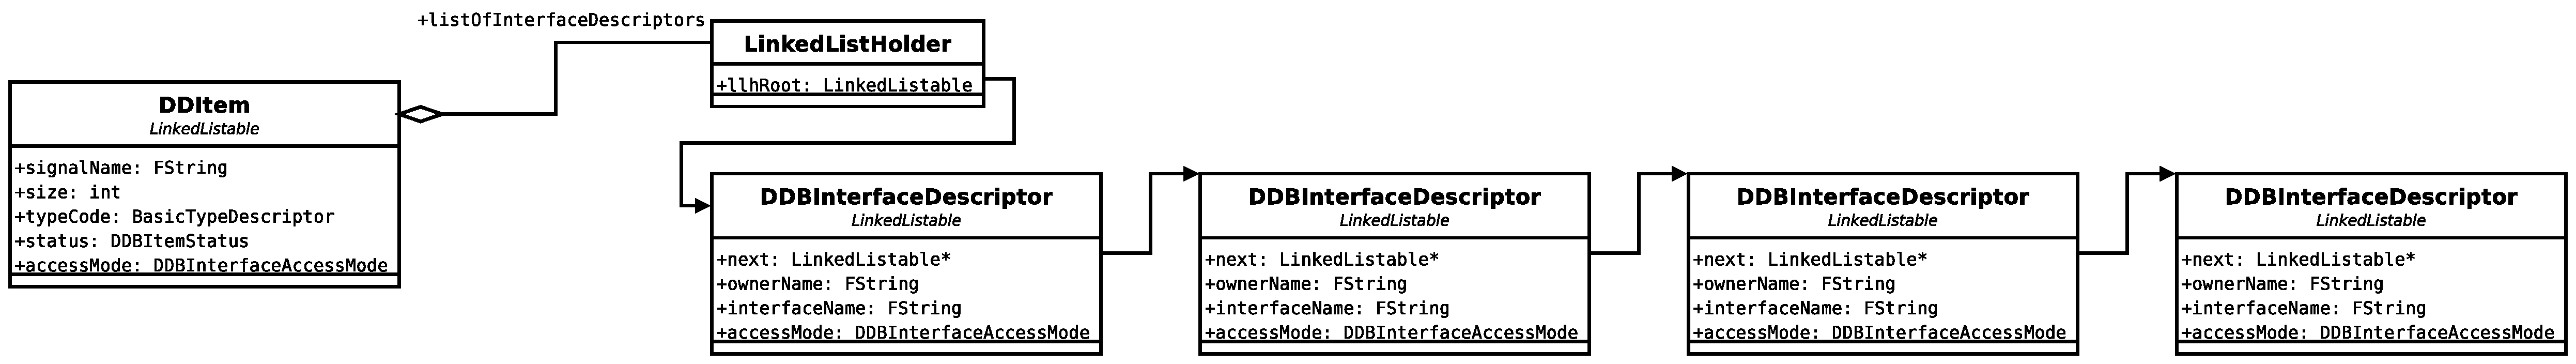
\includegraphics[width=\textwidth]{level5/DDBItem_logic.eps}
  \caption{BaseLib Level 5 DDB, DDBItem UML/logic scheme}
  \label{f:level5:DDB:DDBItem_logic}
 \end{center}
\end{figure}
\begin{figure}[h!]
 \begin{center}
  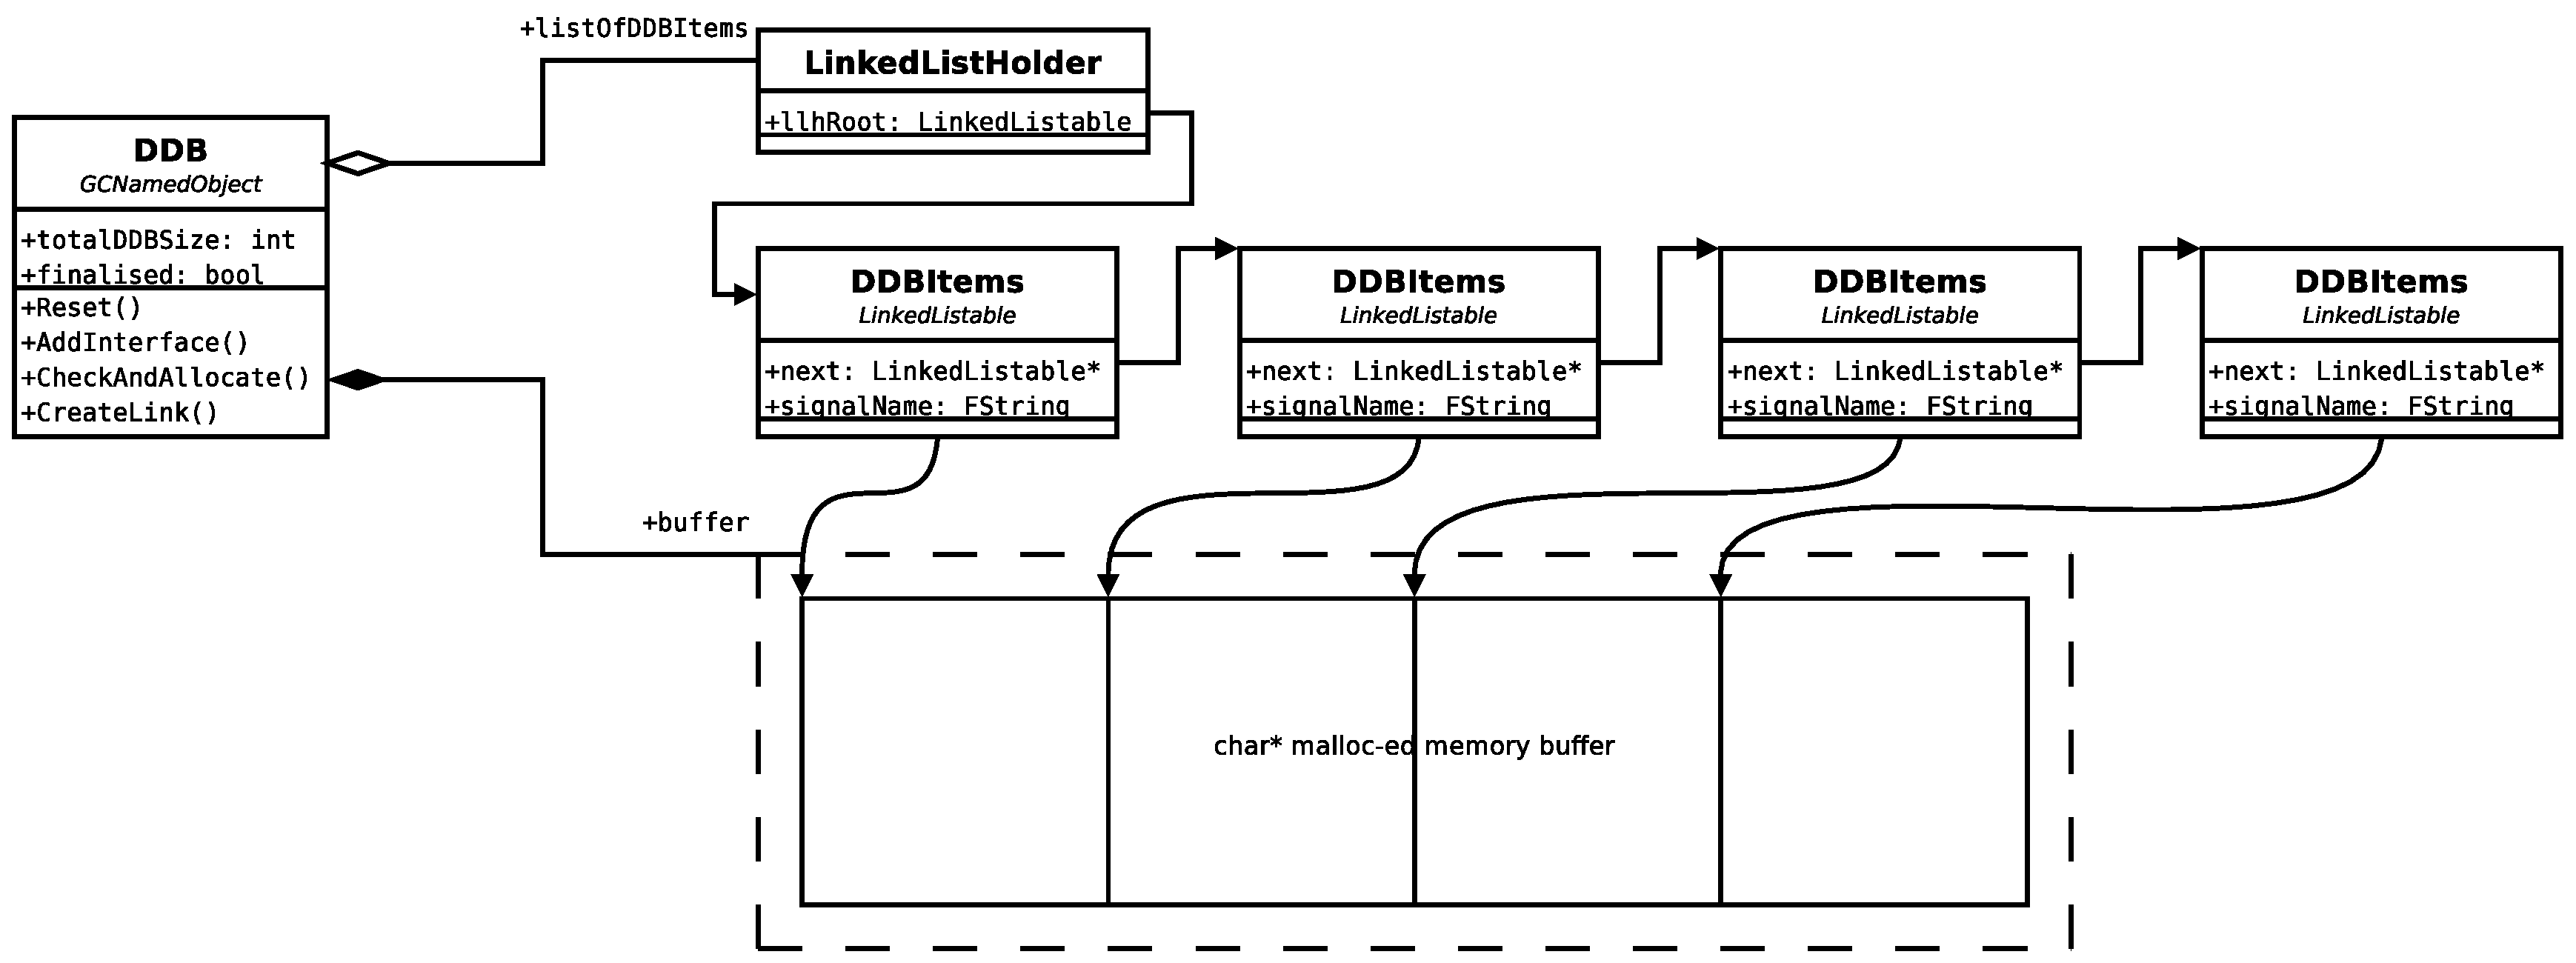
\includegraphics[width=\textwidth]{level5/DDB_logic.eps}
  \caption{BaseLib Level 5 DDB, Dynamic Data Buffer UML/logic scheme}
  \label{f:level5:DDB:DDB_logic}
 \end{center}
\end{figure}

In Figure \ref{f:level5:DDB:DDB_logic} it is possible to see that each \texttt{DDBItem} is associated to a signal and a DDB is a collection of \texttt{DDBItem} (that are collection of \texttt{DDBInterfaceDescriptor}). During the \texttt{DDB::CheckAndAllocate} links between each \texttt{DDBItem} and the memory area buffer are created (i.e. in Figure \ref{f:level5:DDB:DDB_logic} the bezierline's arrows between a \texttt{DDBItem} and the \texttt{buffer}.
Using \texttt{DDB::CreateLink} each one of this information is copied from the correct \texttt{DDBItem} to the \texttt{DataBufferPointer} of a GAM. \\


Once the DDB is ready to use, i.e. each data buffer is correctly assigned, the DDB class is used only to deallocate all the memory space at the end of the program. All the data passing is done by the GAM itself. The DDB bus is used only to allocate and check the memory. \\


In Figure \ref{f:level5:DDB} a whole representation of all the connection between classes in this section is depicted, the UML schema is not exhaustive.

\begin{figure}[h!]
 \begin{center}
  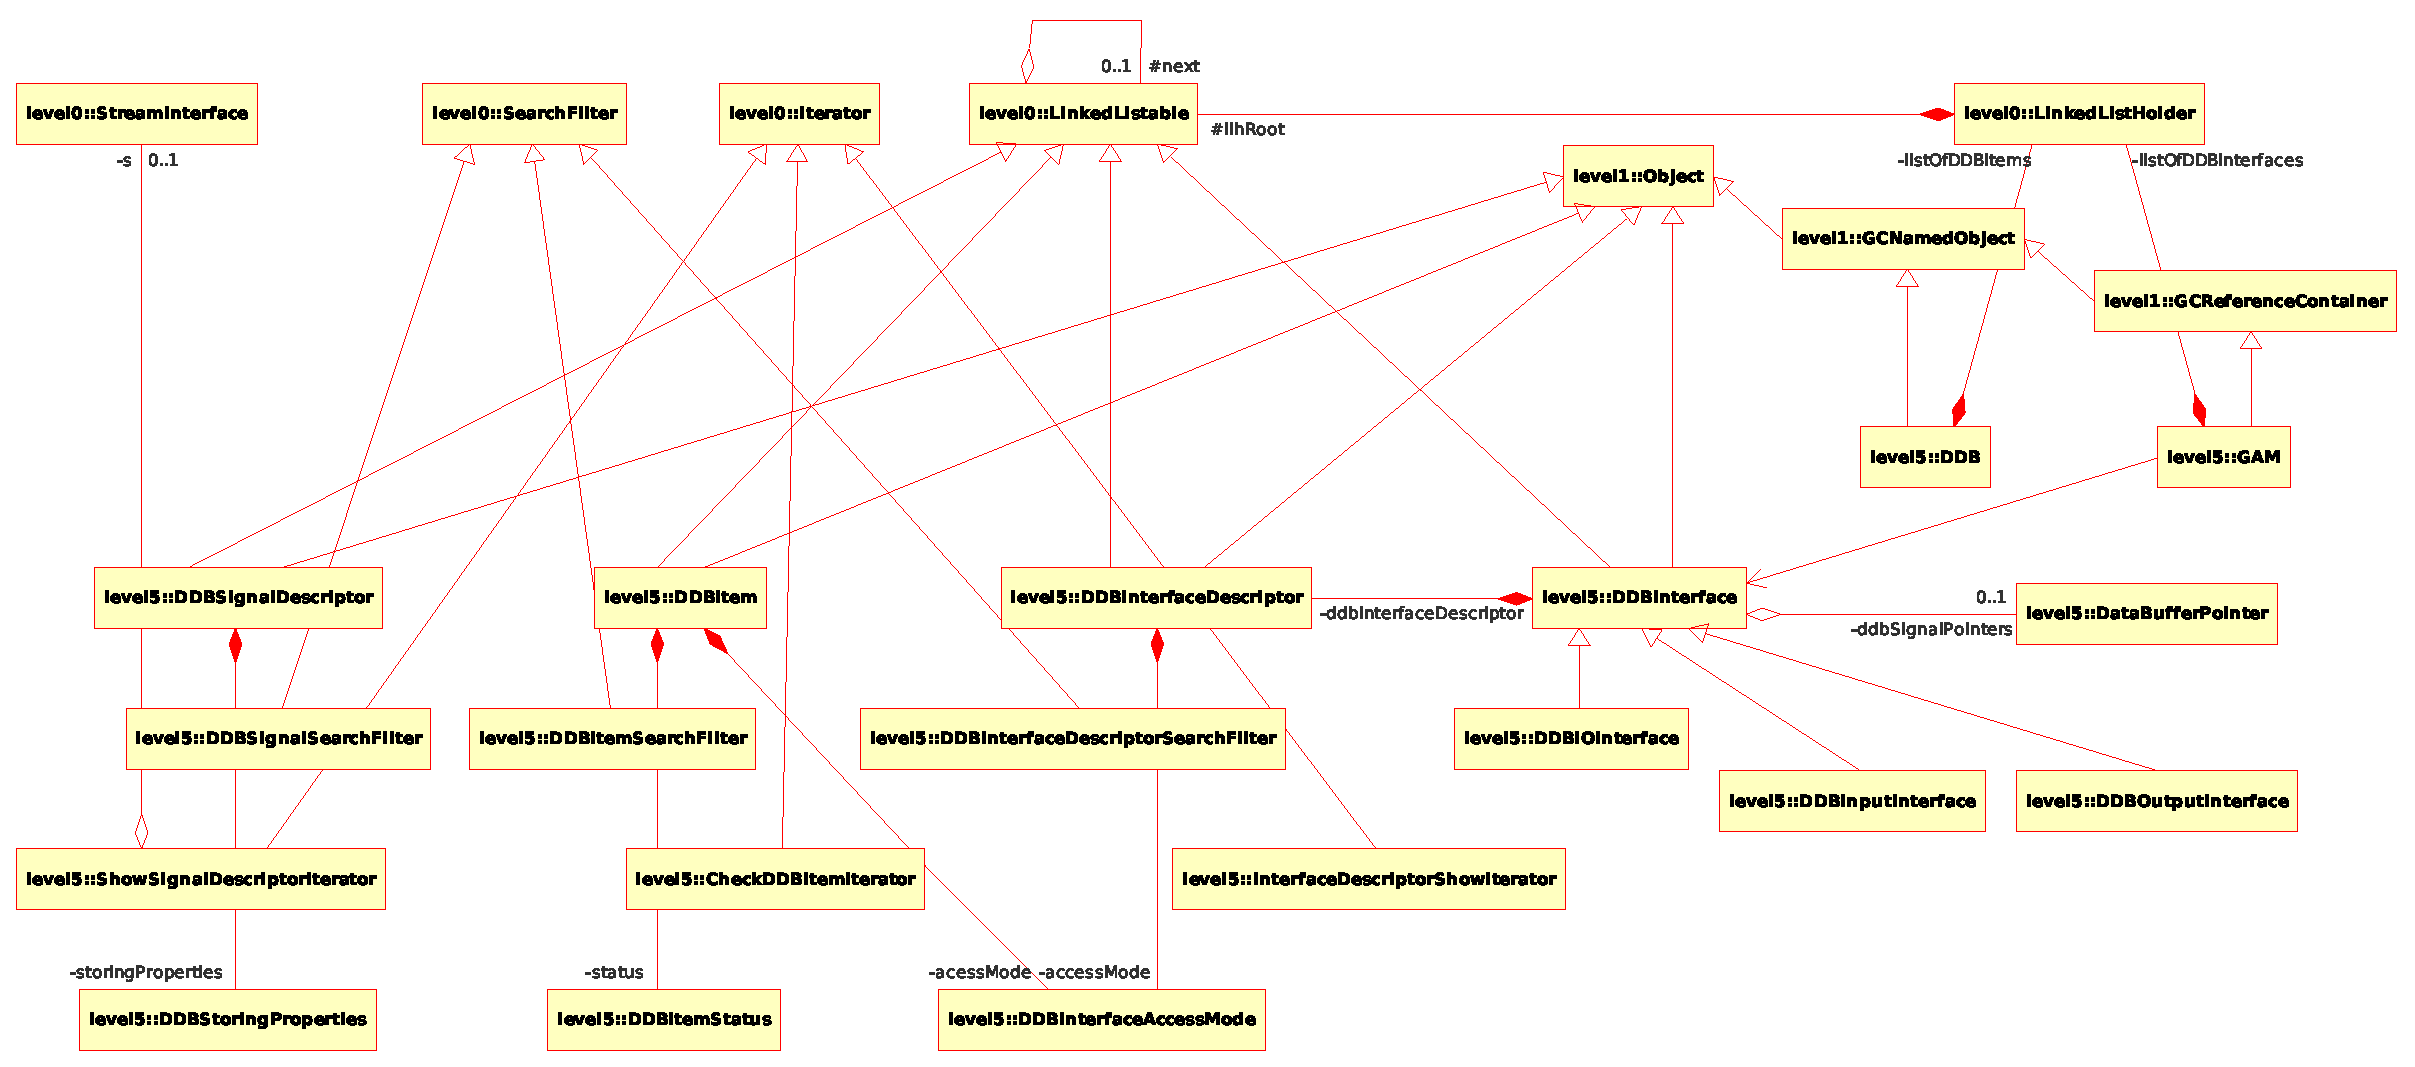
\includegraphics[width=\textwidth]{level5/level5-DDB.eps}
  \caption{BaseLib Level 5 DDB}
  \label{f:level5:DDB}
 \end{center}
\end{figure}

In the following all classes are grouped in two, the first set are classes involved with \texttt{GAM}s and \texttt{DDBInterface}s and the second group examines the DDB internals i.e. the \texttt{DDBItem} and the \texttt{DDB} itself.



\subsection{GAM, DDBInterface}
%Andre articolo
A GAM is a block of code implementing a specific interface specified in the BaseLib2 library. Each GAM contains three communication points: one for configuration and two for data input and output. The core of a typical GAM, processes the input
accordingly to how it was configured and outputs the modified information. The only entry point which is mandatory is the configuration and some GAMs, for instance the ones which interface hardware, are read or write only.

During initialization the modules declare what data they expect to receive and what information is going to be produced in output. Each type of input or output is declared as a configurable named signal with a data type associated. This is the only available way to chain GAMs and provides a clear boundary in the system: GAMs are not aware of other modules. Although GAMs are unrestricted in functionality, the set of GAMs which interface with hardware can be conceptually extracted. These kind of modules are named IOGAMs and provide a unique high level interface to any kind of hardware. The connection between the IOGAM and the specific low level code responsible for driving the hardware is performed through the specialization of a high level class named generic acquisition module. This interface requires the number of hardware inputs and outputs to be specified and forces the existence of a reading and write function. These functions must be implemented for each kind of devices, although it is common that devices belonging to the same family are able to share a common acquisition module. These high level interfaces to the hardware can usually be configured to return the latest acquired value or to wait for a new sample to arrive (at the cost of delaying the execution), depending on the requirements of the application. The most common type of GAMs allow to interface with hardware, store acquired data, execute algorithms, take decisions based on the current state of the system, debug internal states and provide live information about the system.

\begin{figure}[h!]
 \begin{center}
  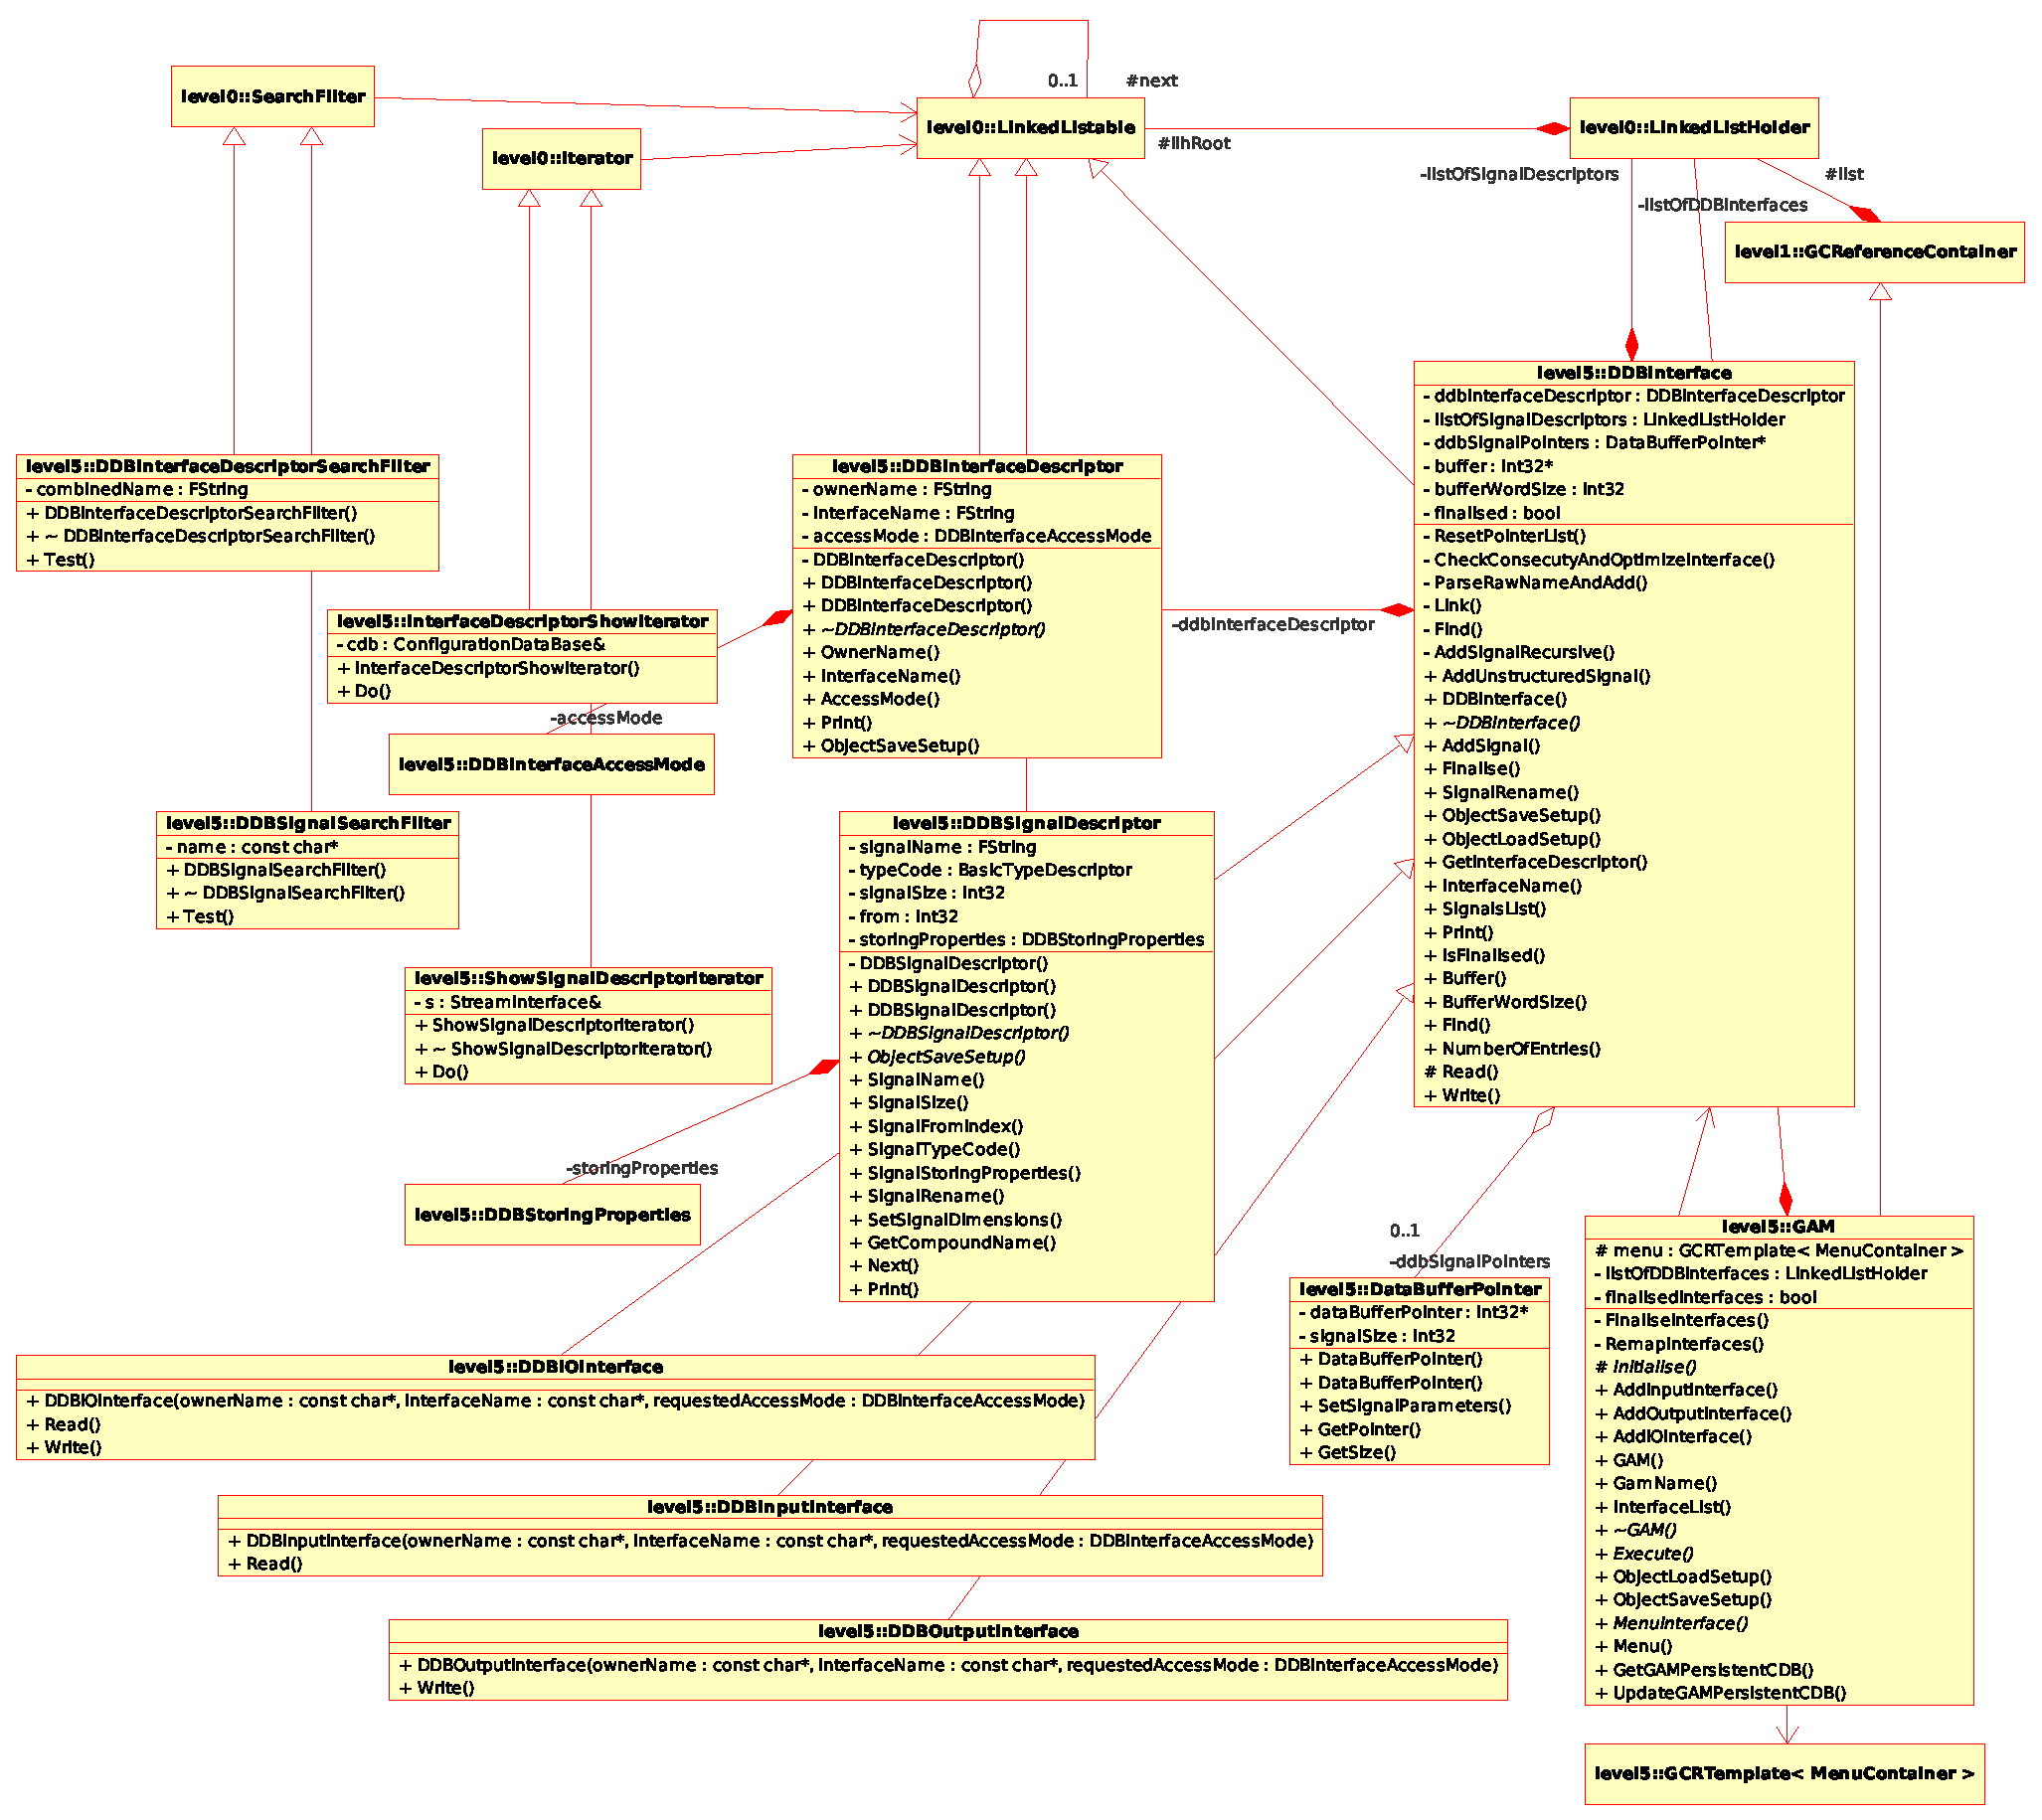
\includegraphics[width=\textwidth]{level5/level5-DDBInterface.eps}
  \caption{BaseLib Level 5 DDB Interface}
  \label{f:level5:DDBInterface}
 \end{center}
\end{figure}

Classes involved in this section are depicted in Figure \ref{f:level5:DDBInterface} and listed below:
\begin{itemize}
 \item DDBStoringProperties
 \item DDBSignalDescriptor, ShowSignalDescriptorIterator, DDBSignalSearchFilter
 \item DDBInterfaceAccessMode
 \item DDBInterfaceDescriptor, InterfaceDescriptorShowIterator, DDBInterfaceDescriptorSearchFilter
 \item DataBufferPointer
 \item DDBInterface
 \item DDBIOInterface, DDBInputInterface, DDBOutputInterface
 \item GAM
\end{itemize}



\subsubsection{DDBStoringProperties}
\texttt{[DDBDefinitions.h, DDBDefinitions.cpp]}\\
The class \texttt{DDBStoringProperties} describes the way data are stored in the DDB. All the possible properties and attributes are stored in the single class's attribute \texttt{properties}, this value codes the property mask.\\


Constructors lets user make a \texttt{DDBStoringProperties} from scratch, from an integer and from another \texttt{DDBStoringProperties}. There are some assignement operators and operators ridefinitions.


The method \texttt{CheckMask} check the object with the passed by object; \texttt{Print} prints on the \texttt{StreamInterface} passed by argument the \texttt{properties} attribute in a human readable form.

\begin{lstlisting}[
extendedchars=true,%
basicstyle=\fontfamily{pcr}\fontseries{m}\selectfont\footnotesize, %
stepnumber=1,%
numberstyle=\tiny,%
keywordstyle=\footnotesize\tt ,%
language=C++]
private:
   int32 properties;

public:
   DDBStoringProperties();
   DDBStoringProperties(const int intProperties);
   DDBStoringProperties(const DDBStoringProperties& reference);

   DDBStoringProperties& operator=(const DDBStoringProperties right);
   DDBStoringProperties& operator|=(const DDBStoringProperties right);
   DDBStoringProperties& operator&=(const DDBStoringProperties right);
   DDBStoringProperties operator~() const;
   bool operator==(const DDBStoringProperties& reference) const;

   bool CheckMask(const DDBStoringProperties& mask) const;
   void Print(StreamInterface& s) const;
\end{lstlisting}

Declared \texttt{DDBStoringProperties} in BaseLib are the following (also declared in \textit{DDBDefinitions.h} as \texttt{const}):

\begin{table}[!h]
 \begin{center}
  \begin{tabular}{|l|c|l|}
   \hline
type & value & description \\
   \hline
\texttt{DDB\_Default} & 0x00 & The signal structure is inserted without using fully qualified names. \\
\texttt{DDB\_FlatNamed} & 0x01 & The signal structure is inserted without using fully qualified names. \\
\texttt{DDB\_Consecutive} & 0x02 & The DDB tries to allocate the signal just next to the previous. \\
\texttt{DDB\_Unsized} & 0x04 & The dimensions of signal are not fully specified. \\
   \hline
  \end{tabular}
 \end{center}
\end{table}



\subsubsection{DDBSignalDescriptor}
\texttt{[DDBSignalDescriptor.h, DDBSignalDescriptor.cpp]}\\
This class is used to represent a signal. It inherits from \texttt{Object} and \texttt{LinkedListable}. The most important attribute is the name of the signal (\texttt{signalName} attribute) of type \texttt{FString}; \texttt{typeCode} codes the type and size of the elementary type used to build this signal.

 \texttt{signalSize} is the actual signal size if the \texttt{from} attribute is $-1$; if it is different this attribute specifies the number of consecutive elements to be read. The attribute \texttt{from} if its different from $-1$ specifies the starting element from which to start reading. \texttt{storingProperties} specifies the storing properties of the signal, i.e. \texttt{DDB\_Default}, \texttt{DDB\_FlatNamed}, \texttt{DDB\_Consecutive} and \texttt{DDB\_Unsized}.
    
\begin{lstlisting}[
extendedchars=true,%
basicstyle=\fontfamily{pcr}\fontseries{m}\selectfont\footnotesize, %
stepnumber=1,%
numberstyle=\tiny,%
keywordstyle=\footnotesize\tt ,%
language=C++]
private:
   FString signalName;
   BasicTypeDescriptor typeCode;
   int32 signalSize;
   int32 from;
   DDBStoringProperties storingProperties;
\end{lstlisting}

The standard contructor has been overridden to avoid silent use; the second constructor is for partially sized signals; this constructor sets the \texttt{DDB\_Unsized} bit overriding the setting made by the user. Then follows the copy contructor and the destructor that just frees the memory allocated during construction.

The method \texttt{ObjectSaveSetup} is the \texttt{DDBSignalDescriptor} save function; it uses a CDB to pass the initialisation parameters; the CDB information is read from the subtree that is currently addressed. \\


Next five methods get signal attributes, the first one returns the name of the signal (\texttt{SignalName}); the method \texttt{SignalSize} gets the number of elements in the signal. \texttt{SignalFromIndex} gets the starting index of the signal. \texttt{SignalTypeCode} returns the type code of the signal and \texttt{SignalStoringProperties} gets the storing properties of the signal. To get the size in byte of the signal the user has to code:
\begin{lstlisting}[
extendedchars=true,%
basicstyle=\fontfamily{pcr}\fontseries{m}\selectfont\footnotesize, %
stepnumber=1,%
numberstyle=\tiny,%
keywordstyle=\footnotesize\tt ,%
language=C++]
sizeof_theSignal = theSignal.SignalSize()*TypeSize(theSignal.SignalTypeCode());
\end{lstlisting}

There are also some setter methods: \texttt{SignalRename} that sets the name of the signal and \texttt{SetSignalDimensions} that sets the number of \texttt{maxDimensions} of the signal.

The class ends with some utility functions; the method \texttt{GetCompoundName} returns the signal name with added informations, if the signal is unsized it returns the element/s to be used withing round brackets, if the signal is sized it returns the signal name with the dimension within square brackets. \texttt{Next} calls \texttt{LinkedListable::Next} and \texttt{Print} simply prints the content.

\begin{lstlisting}[
extendedchars=true,%
basicstyle=\fontfamily{pcr}\fontseries{m}\selectfont\footnotesize, %
stepnumber=1,%
numberstyle=\tiny,%
keywordstyle=\footnotesize\tt ,%
language=C++]
   DDBSignalDescriptor();
public:
   inline DDBSignalDescriptor(const char* signalName,const int signalSize,
       const int from,const BasicTypeDescriptor typeCode,const DDBStoringProperties& ddbss);
   inline DDBSignalDescriptor(const DDBSignalDescriptor& descriptor);
   virtual ~DDBSignalDescriptor();

   virtual bool ObjectSaveSetup(ConfigurationDataBase& info,StreamInterface* err) const;

public:
   const char* SignalName() const;
   int32 SignalSize() const;
   int32 SignalFromIndex() const;
   BasicTypeDescriptor SignalTypeCode() const;
   DDBStoringProperties SignalStoringProperties() const;

   void SignalRename(const char* newSignalName);
   void SetSignalDimensions(const int signalSize);

   bool GetCompoundName(FString& compoundName);
   DDBSignalDescriptor* Next() const;

   void Print(StreamInterface& s)const;
\end{lstlisting}

Remember from the introduction of this section that a \texttt{DDBSignalDescription} is the description of a signal and is not directly bounded to signal data itself, data and pointers to signal data are accounted by an associated \texttt{DataBufferPointer} structure.



\subsubsection{ShowSignalDescriptorIterator}
\texttt{[DDBSignalDescriptor.h]}\\
This is the iterator for a list of \texttt{DDBSignalDescriptor}s. It inherits from \texttt{Iterator} and simple iterate through \texttt{DDBSignalDescriptor}s and prints its content on the \texttt{StreamInterface} attribute.

This function uses the C++'s dynamic cast operator.

\begin{lstlisting}[
extendedchars=true,%
basicstyle=\fontfamily{pcr}\fontseries{m}\selectfont\footnotesize, %
stepnumber=1,%
numberstyle=\tiny,%
keywordstyle=\footnotesize\tt ,%
language=C++]
private:
   StreamInterface& s;

public:
   ShowSignalDescriptorIterator(StreamInterface& si);
   virtual ~ShowSignalDescriptorIterator();

   void Do(LinkedListable* ll);
\end{lstlisting}



\subsubsection{DDBSignalSearchFilter}
\texttt{[DDBSignalDescriptor.h]}\\
This class is a search filter used to find a \texttt{DDBSignalDescriptor} by name in a list of \texttt{DDBSignalDescriptor}s (for example \texttt{DDBInterface::listOfSignalDescriptors}). It inherits from \texttt{SearchFilter}.

The single attribute that must be initialized by the constructor is the signal name to be searched.

\begin{lstlisting}[
extendedchars=true,%
basicstyle=\fontfamily{pcr}\fontseries{m}\selectfont\footnotesize, %
stepnumber=1,%
numberstyle=\tiny,%
keywordstyle=\footnotesize\tt ,%
language=C++]
private:
   const char* name;

public:
   DDBSignalSearchFilter(const char* name);
   virtual ~DDBSignalSearchFilter();

   bool Test(LinkedListable* ll);
\end{lstlisting}



\subsubsection{DDBInterfaceAccessMode}
\texttt{[DDBDefinitions.h, DDBDefinitions.cpp]}\\
The class \texttt{DDBInterfaceAccessMode} defines the the DDB access mode. The structure actually contains two conceptually different variables: the first is a code for the type of \texttt{DDBInterface} (as we will see there are input, output and IO DDB interfaces) used by its owner (and it really is an access mode to the DDB); the second represent the state of the DDB while adding interfaces and is used to detect errors. Users can access the DDB using five different interfaces or modalities:

\begin{itemize}
 \item a placeholder.
 \item As a reader.
 \item As a writer.
 \item As a patcher.
 \item As an exclusive writer.
\end{itemize}

TODO\\
TODO\\
TODO\\
spiegare meglio le differenze

These access modes are encoded by a number of bits in a \texttt{DDBAccessMode} variable as shown in the following table.

\begin{table}[!h]
 \begin{center}
  \begin{tabular}{|l|c|c|c|c|}
   \hline
\textbf{Access Type} & \textbf{R} & \textbf{W} & \textbf{P} & \textbf{E} \\
   \hline
Placeholder & 0 & 0 & 0 & 0 \\
Reader & 1 & 0 & 0 & 0 \\
Writer & 0 & 1 & 0 & 0 \\
Patcher & 0 & 0 & 1 & 0 \\
Exclusive Writer & 0 & 1 & 0 & 1 \\
   \hline
  \end{tabular}
 \end{center}
\end{table}

Different users however (and also a single user), can access the same signal using different interfaces provided that they are compatible. Below it is shown the table of the compatible interfaces.

\begin{table}[!h]
 \begin{center}
  \begin{tabular}{|l|c|c|c|c|}
   \hline
\textbf{Access Type} & \textbf{R} & \textbf{W} & \textbf{P} & \textbf{E} \\
   \hline
Reader and Writer & 1 & 1 & 0 & 0 \\
Reader and Exclusive Writer & 1 & 0 & 0 & 1 \\
Reader and Patcher & 1 & 0 & 1 & 0 \\
Writer and Patcher & 0 & 1 & 1 & 0 \\
Reader, Writer and Patcher & 1 & 1 & 1 & 0 \\
   \hline
  \end{tabular}
 \end{center}
\end{table}

All of the other bits combinations are not valid. In particular it is worth noticing that if \texttt{E} is set also \texttt{W} is set.
In a \texttt{DDBItem} object, where a list of users of the same signal is managed, the following access rules apply:

\begin{itemize}
 \item Either there must be a user having the Writer access to the signal or all the users being Placeholders.
 \item No more than one user can have the Writer or Exclusive Writer access to that signal.
 \item If the writer has has the Exclusive Writer access the other users can't get the Patcher access.
\end{itemize}

The class \texttt{DDBInterfaceAccessMode} live around a single attribute \texttt{mode} that codes the access mode. There are three constructors: the standard constructor initialises to \texttt{DDB\_PlaceholderMode}, a constructor from integer and the copy constructor.
The assignment operator, the bitwise or, and, not and the equal operator are defined to make operations easier.

The method \texttt{CheckMask} compare the object itself with the object passed by.
\texttt{ObjectSaveSetup} saves parameters to CDB.
\begin{lstlisting}[
extendedchars=true,%
basicstyle=\fontfamily{pcr}\fontseries{m}\selectfont\footnotesize, %
stepnumber=1,%
numberstyle=\tiny,%
keywordstyle=\footnotesize\tt ,%
language=C++]
   int mode;

public:
   DDBInterfaceAccessMode();
   DDBInterfaceAccessMode(const int intMode);
   DDBInterfaceAccessMode(const DDBInterfaceAccessMode& reference);

   DDBInterfaceAccessMode& operator=(const DDBInterfaceAccessMode& right);
   DDBInterfaceAccessMode& operator|=(const DDBInterfaceAccessMode& right);
   DDBInterfaceAccessMode& operator&=(const DDBInterfaceAccessMode& right);
   DDBInterfaceAccessMode operator~() const;
   bool operator==(const DDBInterfaceAccessMode& reference) const;

   bool CheckMask(const DDBInterfaceAccessMode& mask) const;

   void Print(StreamInterface& s) const;

   bool ObjectSaveSetup(ConfigurationDataBase& info, StreamInterface* err)const;
\end{lstlisting}

In BaseLib are defined the following \texttt{DDBInterfaceAccessMode}s:

\begin{table}[!h]
 \begin{center}
  \begin{tabular}{|l|c|l|}
   \hline
type & value & description \\
   \hline
\texttt{DDB\_PlaceholderMode} & 0x00 & The value of the Placeholder. \\
\texttt{DDB\_ReadMode} & 0x01 & The value of the ReadMode. \\
\texttt{DDB\_WriteMode} & 0x02 & The value of the WriteMode. \\
\texttt{DDB\_PatchMode} & 0x04 & The value of the PatchMode. \\
\texttt{DDB\_ExclusiveWriteMode} & 0x0a & The value of the WriteExclusive. \\
\texttt{DDB\_ExclusiveWriteBit} & 0x08 & The mask for the value of the bit WriteExclusive. \\
   \hline
  \end{tabular}
 \end{center}
\end{table}



\subsubsection{DDBInterfaceDescriptor}
\texttt{[DDBInterfaceDescriptor.h, DDBInterfaceDescriptor.cpp]}\\
The class \texttt{DDBInterfaceDescriptor} inherits from \texttt{LinkedListable} and \texttt{Object}. Implements a user of the DDB.

The attribute \texttt{ownerName} is the name of the user (GAM). In this context user means both GAMs for which the signal is an input and those for which the signal is an output. The attribute \texttt{interfaceName} is the name of the \texttt{DDBInterface} holding the class. \texttt{accessMode} specifies the \texttt{DDBInterface} access mode to the signals.

\begin{lstlisting}[
extendedchars=true,%
basicstyle=\fontfamily{pcr}\fontseries{m}\selectfont\footnotesize, %
stepnumber=1,%
numberstyle=\tiny,%
keywordstyle=\footnotesize\tt ,%
language=C++]
private:
   FString ownerName;
   FString interfaceName;
   DDBInterfaceAccessMode accessMode;
\end{lstlisting}

The standard constructor is disabled, i.e. its private. The next constructor is the only one that can be safely called in the constructor of a derived class to initialise the parent, then the copy constructor follows. With this trick it is possible to create a new DDBInterfaceDescriptor only copying it from a derived class, or creating it from scratch with all the parameters.

Some getter methods follows that let you know the name of the owner of the interface, the name of the interface itself and the access mode.
\begin{lstlisting}[
extendedchars=true,%
basicstyle=\fontfamily{pcr}\fontseries{m}\selectfont\footnotesize, %
stepnumber=1,%
numberstyle=\tiny,%
keywordstyle=\footnotesize\tt ,%
language=C++]
   DDBInterfaceDescriptor();

public:
   DDBInterfaceDescriptor(const char* ownerName,const char* interfaceName,
      const DDBInterfaceAccessMode accessMode);
   DDBInterfaceDescriptor(const DDBInterfaceDescriptor& descriptor);
   virtual ~DDBInterfaceDescriptor();

   const char* OwnerName() const;
   const char* InterfaceName() const;
   const DDBInterfaceAccessMode& AccessMode() const;

   void Print(StreamInterface& s) const;

   bool ObjectSaveSetup(ConfigurationDataBase& info, StreamInterface* err);
\end{lstlisting}



\subsubsection{InterfaceDescriptorShowIterator}
\texttt{[DDBInterfaceDescriptor.h]}\\
The class \texttt{InterfaceDescriptorShowIterator} implements the \texttt{ObjectSaveSetup} method for all members of a \texttt{DDBInterfaceDescriptor}'s list. It inherits from \texttt{Iterator}. It works on a CDB, infact the only attribute is a reference to a \texttt{ConfigurationDataBase}.

\begin{lstlisting}[
extendedchars=true,%
basicstyle=\fontfamily{pcr}\fontseries{m}\selectfont\footnotesize, %
stepnumber=1,%
numberstyle=\tiny,%
keywordstyle=\footnotesize\tt ,%
language=C++]
private:
   ConfigurationDataBase& cdb;

public:
   InterfaceDescriptorShowIterator(ConfigurationDataBase& cdbi);
   void Do(LinkedListable* ll);
\end{lstlisting}



\subsubsection{DDBInterfaceDescriptorSearchFilter}
\texttt{[DDBInterfaceDescriptor.h]}\\
This is an ancillary class used to serch a \texttt{DDBInterfaceDescriptor}'s list. Class \texttt{DDBInterfaceDescriptorSearchFilter} inherits from \texttt{SearchFilter}.
The only attribute \texttt{combinedName} is the identifier to look for.

\begin{lstlisting}[
extendedchars=true,%
basicstyle=\fontfamily{pcr}\fontseries{m}\selectfont\footnotesize, %
stepnumber=1,%
numberstyle=\tiny,%
keywordstyle=\footnotesize\tt ,%
language=C++]
private:
   FString combinedName;

public:
   DDBInterfaceDescriptorSearchFilter(const char* gamName,const char* interfaceName);
   virtual ~DDBInterfaceDescriptorSearchFilter();

   bool Test(LinkedListable* ll);
\end{lstlisting}



\subsubsection{DataBufferPointer}
\texttt{[DDBInterface.h, DDBInterface.cpp]}\\
The class \texttt{DataBufferPointer} containes the \texttt{int32} pointer to the memory where the signal is stored. It contains also the \texttt{signalSize}, where the size is the number of \texttt{int32} elements that are to be read. A \texttt{DataBufferPointer} is associated to a single \texttt{DDBSignalDescriptor} in a \texttt{DDBInterface}.\\


A \texttt{DataBufferPointer} can be set via the constructor (the second) or via the \texttt{SetSignalParameters} method. The last two methods return the attributes.

\begin{lstlisting}[
extendedchars=true,%
basicstyle=\fontfamily{pcr}\fontseries{m}\selectfont\footnotesize, %
stepnumber=1,%
numberstyle=\tiny,%
keywordstyle=\footnotesize\tt ,%
language=C++]
private:
   int32* dataBufferPointer;
   int32 signalSize;

public:
   DataBufferPointer();
   DataBufferPointer(int32* dataBufferPointer,int32 signalSize);
   void SetSignalParameters(int32* dataBufferPointer,int32 signalSize);

   int32* GetPointer() const;
   int32 GetSize() const;
\end{lstlisting}



\subsubsection{DDBInterface}
\texttt{[DDBInterface.h, DDBInterface.cpp]}\\
Many \texttt{DDBInterface}s build up a single GAM. A \texttt{DDBInterface} is build around the access method is being used to collect data. Signals with the same access mode should be grouped and accessed in a unique operation for efficiency. It inherits from \texttt{Object} and \texttt{LinkedListable}. \\

The attribute \texttt{ddbInterfaceDescriptor} describes the properties of the interface, i.e. the interface name, the GAM owner and the access mode to the signals in the DDB.
The attribute \texttt{listOfSignalDescriptors} is a list of \texttt{DDBSignalDescriptor}s, this list should be made by all the signals accessed by the user with the specified access mode.
The attribute \texttt{ddbSignalPointers} is an array of pointers to specific DDB signals.
\texttt{buffer} is a pointer to the working buffer of this interface. \texttt{buffeWordSize} is the size in \texttt{int32} of \texttt{buffer}.
The last attribute, \texttt{finalised}, is \texttt{true} when the \texttt{DDBInterface} can be linked to the DDB.
\begin{lstlisting}[
extendedchars=true,%
basicstyle=\fontfamily{pcr}\fontseries{m}\selectfont\footnotesize, %
stepnumber=1,%
numberstyle=\tiny,%
keywordstyle=\footnotesize\tt ,%
language=C++]
private:
   DDBInterfaceDescriptor ddbInterfaceDescriptor;
   LinkedListHolder listOfSignalDescriptors;
   DataBufferPointer* ddbSignalPointers;
   int32* buffer;
   int32 bufferWordSize;
   bool finalised;
\end{lstlisting}
   
The method \texttt{ResetPointerList} resets the pointer list. It should only be called by a DDB class to allow reinitialization.
The method \texttt{CheckConsecutyAndOptimizeInterface} should be called by the DDB after having added the interface; it looks into the \texttt{ddbSignalPointers} array for consecutive elements; if consecutive elements are found, only one pointer with an increased number of elements is used; return \texttt{True} if everything goes well \texttt{False} if the interface has not been finalized.
The method \texttt{ParseRawNameAndAdd} checks if the signal name has the interval extension as in the \texttt{rawName} parameter; if the signals name is specified with square brackets thenction assumes that the number specified within brackets is the signals size (i.e. A[5] is a signal of name A of size 5). If the signal is specified with round brackets the function assumes that the numbers specify the elements that are to be used; valid sintax are A(4), A(1,3,4,6), A(4:6) and A(2:4,7:9). If the user specifies the signal with round brackets the storing properties of the signal are set to \texttt{DDB\_Unsized}. Only interface with read access can use the range specifications. \\


The method \texttt{Link} is used to initialise the pointers to the DDB buffer. This function has to be called from the DDB who is the only one entity that can assign meaningful pointers and sizes, the parameter \texttt{signalName} is the name of the signal to link, \texttt{ddbSignalPointer} is the pointer of the signal in the DDB, it returns \texttt{True} if it has been successfull, \texttt{False} otherwise.
The method \texttt{Find} finds by name a signal in the \texttt{listOfSignalDescriptors} starting from \texttt{index} element in the list, returns the descriptor which matches the \texttt{signalName}.
The method \texttt{AddSignalRecursive} adds structured signals to the \texttt{DDBInterface}. The method \texttt{AddUnstructuredSignal} adds basic type signals to the \texttt{DDBInterface}. \\

\begin{lstlisting}[
extendedchars=true,%
basicstyle=\fontfamily{pcr}\fontseries{m}\selectfont\footnotesize, %
stepnumber=1,%
numberstyle=\tiny,%
keywordstyle=\footnotesize\tt ,%
language=C++]
   bool ResetPointerList();
   bool CheckConsecutyAndOptimizeInterface();
   bool ParseRawNameAndAdd(const char* rawName,const char* signalType,
      DDBStoringProperties& properties);

   bool Link(const char* signalName,int32* ddbSignalPointer);
   DDBSignalDescriptor* Find(const char* signalName,uint32& index);
   bool AddSignalRecursive(const char* signalName,const char* signalType,
      int signalSize,int from,DDBStoringProperties& properties);
   bool AddUnstructuredSignal(const char* signalName,const int signalSize,
      const int from,const BasicTypeDescriptor typeCode,DDBStoringProperties& properties);
\end{lstlisting}

Then comes a constructor, parameter \texttt{ownerName} is the name of the GAM that owns the \texttt{DDBInterface}, \texttt{interfaceName} is the name of the interface and \texttt{requestedAccessMode} specifies the access mode of the interface to the DDB. A destructor follows. \\


The public method \texttt{AddSignal} adds a structured type signal, param \texttt{signalName} is the name of the signal, \texttt{signalType} is the type of the signal and param \texttt{properties} specifies the storing properties of the signal. The method \texttt{Finalise} allocates memory for the DDB read and/or write operations and put the interface in a status which stops accepting new signals. \\


The method \texttt{SignalRename} renames all occurences of signal ``signalName'' in the \texttt{listOfSignalDescriptors} list with the name ``newSignalName''. \texttt{ObjectSaveSetup} and \texttt{ObjectLoadSetup} saves the \texttt{DDBInterface} to a DDB and initialize the \texttt{DDBInterface}. \\


Then follows a great number of getter methods. The method \texttt{GetInterfaceDescriptor} returns the \texttt{DDBInterfaceDescriptor}; \texttt{InterfaceName} returns the interface name; \texttt{SignalsList} returns the first element in the \texttt{listOfSignalDescriptors} attribute; \texttt{Print} is the print method. The method \texttt{IsFinalised} checks if the DDB is finalised, \texttt{True} if its finalised, \texttt{False} otherwise; \texttt{Buffer} returns the \texttt{buffer} attribute; the method \texttt{BufferWordSize} returns the number of float/int32 signals that are stored in the buffer; if this method is called before the interface has been finalised it returns the buffer size of the added signal list. Otherwise it returns the buffer size, the returned value is greater or equal of the value returned from the \texttt{NumberOfEntries} method. \\


The method \texttt{Find} returns a pointer to a \texttt{DDBSignalDescriptor} of a signal identified by name ``signalName'' in the \texttt{DDBInterface}. The method \texttt{NumberOfEntries} returns the number of entries in the \texttt{listOfSignalDescriptors} list. This can be different from the BufferWordSize if any of the signal in the List has a size larger than one. \\


The last two protected methods are fast method to read and write to the data buffer.

\begin{lstlisting}[
extendedchars=true,%
basicstyle=\fontfamily{pcr}\fontseries{m}\selectfont\footnotesize, %
stepnumber=1,%
numberstyle=\tiny,%
keywordstyle=\footnotesize\tt ,%
language=C++]
public:
   DDBInterface(const char* ownerName,const char* interfaceName,
      DDBInterfaceAccessMode requestedAccessMode);
   virtual ~DDBInterface();

   bool AddSignal(const char* signalName,const char* signalType,
      DDBStoringProperties properties=DDB_Default);
   bool Finalise();
   bool SignalRename(const char* signalName,const char* newSignalName);

   bool ObjectSaveSetup(ConfigurationDataBase& info,StreamInterface* err);
   bool ObjectLoadSetup(ConfigurationDataBase& info,StreamInterface* err);

   const DDBInterfaceDescriptor& GetInterfaceDescriptor();
   const char* InterfaceName() const;
   const DDBSignalDescriptor* SignalsList() const;

   void Print(StreamInterface& s) const;
   bool IsFinalised() const;

   int32* Buffer();
   int32 BufferWordSize() const;

   const DDBSignalDescriptor* Find(const char* signalName) const;
   int32 NumberOfEntries() const;

protected:
   inline void Read();
   inline void  Write();
\end{lstlisting}



\subsubsection{DDBInputInterface}
\texttt{[DDBInputInterface.h]}\\
The \texttt{DDBInputInterface} is one of the three class that inherits from \texttt{DDBInterface}; it represents an input interface, i.e. a data producer, infact the only implemented method is the \texttt{Read} method. This class must be extended from a user.
\begin{lstlisting}[
extendedchars=true,%
basicstyle=\fontfamily{pcr}\fontseries{m}\selectfont\footnotesize, %
stepnumber=1,%
numberstyle=\tiny,%
keywordstyle=\footnotesize\tt ,%
language=C++]
public:
   DDBInputInterface(
      const char* ownerName, const char* interfaceName,
      DDBInterfaceAccessMode requestedAccessMode) :
         DDBInterface(ownerName, interfaceName, requestedAccessMode){};

    inline void Read();
\end{lstlisting}



\subsubsection{DDBOutputInterface}
\texttt{[DDBOutputInterface.h]}\\
The \texttt{DDBOutputInterface} is one of the three class that inherits from \texttt{DDBInterface}; it represents an output interface, i.e. a data consumer, infact the only implemented method is the \texttt{Write} method. This class must be extended from a user.
\begin{lstlisting}[
extendedchars=true,%
basicstyle=\fontfamily{pcr}\fontseries{m}\selectfont\footnotesize, %
stepnumber=1,%
numberstyle=\tiny,%
keywordstyle=\footnotesize\tt ,%
language=C++]
public:
   DDBOutputInterface(
      const char* ownerName, const char* interfaceName,
      DDBInterfaceAccessMode requestedAccessMode) :
         DDBInterface(ownerName, interfaceName, requestedAccessMode){};

   inline void Write();
\end{lstlisting}



\subsubsection{DDBIOInterface}
\texttt{[DDBIOInterface.h]}\\
The class \texttt{DDBIOInterface} is the last class that inherits from \texttt{DDBInterface}.
It implements the input and the output interface at the same time.
\begin{lstlisting}[
extendedchars=true,%
basicstyle=\fontfamily{pcr}\fontseries{m}\selectfont\footnotesize, %
stepnumber=1,%
numberstyle=\tiny,%
keywordstyle=\footnotesize\tt ,%
language=C++]
public:
   DDBIOInterface(
      const char* ownerName, const char* interfaceName,
      DDBInterfaceAccessMode requestedAccessMode) :
         DDBInterface(ownerName, interfaceName, requestedAccessMode);

   inline void Read();
   inline void Write();
\end{lstlisting}



\subsubsection{GAM}
\texttt{[GAM.h, GAM.cpp]}\\
This class is the interface of a Generic Acquisition Module (GAM) in the conceptual sense (i.e. not an interface in the OOP meaning). A GAM inherits from \texttt{GCReferenceContainer}. The first attribute is of type \texttt{GCRTemplate<MenuContainer>} and is the Menu Interface for the GAM, it is initialized after the \texttt{FinaliseInterface} method is called. The attribute \texttt{listOfDDBInterfaces} is a container of interfaces within the DDB. The attribute \texttt{finalisedInterfaces} accounts if the GAM is finalised or not.

\begin{lstlisting}[
extendedchars=true,%
basicstyle=\fontfamily{pcr}\fontseries{m}\selectfont\footnotesize, %
stepnumber=1,%
numberstyle=\tiny,%
keywordstyle=\footnotesize\tt ,%
language=C++]
protected:
   GCRTemplate<MenuContainer> menu;

private:
   LinkedListHolder listOfDDBInterfaces;
   bool finalisedInterfaces;
\end{lstlisting}

The method \texttt{FinaliseInterfaces} finalises all \texttt{DDBInterface}s in the attribute \texttt{listOfDDBInterfaces}; it parses all interfaces, sets each interface in a state that does not allow adding or modifying signals, and allocates the memory for storing the signals, returns \texttt{True} if everything was fine; \texttt{False} otherwise.
The method \texttt{RemapInterfaces} renames some or all signals in the \texttt{DDBInterface}s to the value specified in the CDB; the code checks for the presence of a field ``Remappings''. If this field is found, the code checks in this subtree for an entry with the same name of one of the interfaces; if the interface name is found, the code parses all the fields in the subtree. The name of the entry has to be the name of a signal contained in the interface, the value associated to the entry name is the new name that is used for the signal. Then follow an example of configuration file:

\begin{lstlisting}[
extendedchars=true,%
basicstyle=\fontfamily{pcr}\fontseries{m}\selectfont\footnotesize, %
stepnumber=1,%
numberstyle=\tiny,%
keywordstyle=\footnotesize\tt ,%
language=bash]
  Remappings = {
    InputInterface = {
      OldSignalName = NewSignalName
      ...
    }
    OutputInterface = {
      OldSignalName = NewSignalName
      ...
    }
  }
\end{lstlisting}

The method \texttt{Initialise} is called by the executor during the \texttt{ObjectLoadSetup} process, it initialises the GAM parameters and add interfaces to the list.
The method \texttt{AddInputInterface} allows the user to add a \texttt{DDBInputInterface} in the list, the interface created will have only the \texttt{DDB\_ReadMode} access and this cannot be changed.
The method \texttt{AddOutputInterface} allows the user to add a \texttt{DDBOutputInterface} in the list, by default the interface has only the \texttt{DDB\_WriteMode} access, anyway other access modes can be used with the exception of the read mode, the \texttt{DDB\_ReadMode} bit is always cleared before construction.
The method \texttt{AddIOInterface} allows the user to add a \texttt{DDBIOInterface} in the list, by default the interface has the \texttt{DDB\_ReadMode} and \texttt{DDB\_WriteMode} access, all the other access modes can freely be used.

\begin{lstlisting}[
extendedchars=true,%
basicstyle=\fontfamily{pcr}\fontseries{m}\selectfont\footnotesize, %
stepnumber=1,%
numberstyle=\tiny,%
keywordstyle=\footnotesize\tt ,%
language=C++]
   bool FinaliseInterfaces();
   bool RemapInterfaces(ConfigurationDataBase& cdbData);

protected:
   virtual bool Initialise(ConfigurationDataBase& cdbData)=0;

public:
   inline bool AddInputInterface(DDBInputInterface*& ddbi,const char* interfaceName);
   inline bool AddOutputInterface(DDBOutputInterface*& ddbo, const char* interfaceName,
      DDBInterfaceAccessMode accessMode=DDB_WriteMode);
   inline bool AddIOInterface(DDBIOInterface*& ddbio,const char* interfaceName,
      DDBInterfaceAccessMode accessMode=DDB_ReadMode|DDB_WriteMode);
\end{lstlisting}

The method \texttt{GamName} returns the name of the GAM, \texttt{InterfacesList} gets the list of interfaces used by the GAM.
The method \texttt{Execute} is called by the executor (i.e. MARTe) when appropriate. The user can (has to) take different actions depending on the value of the parameter passed, values supperted are:


\begin{table}[!h]
 \begin{center}
  \begin{tabular}{|l|c|l|}
   \hline
name & value & description \\
   \hline
\texttt{GAMPrepulse} & 0x00000001 & Called once before going online. \\
\texttt{GAMOffline} & 0x00000002 & Called continuously while offline. \\ 
\texttt{GAMSafety} & 0x00000003 & Called continuously after a fault has been detected. \\
\texttt{GAMCheck} & 0x00000004 & Called once to verify if the parameter configuration is acceptable. \\
\texttt{GAMPostpulse} & 0x00000005 & Called once before going online. \\
\texttt{GAMStartUp} & 0x00000006 & Called once before going online. \\
\texttt{GAMOnline} & 0x00010000 & Called continuously when online after data has been read. \\
\texttt{GAMOnline2} & 0x00010001 & Called continuously when online after data has been written \\
 & & (but before writing the JPF). User defined functions starts from this offset. \\
   \hline
  \end{tabular}
 \end{center}
\end{table}

User defined functions are GAMOnline3, GAMOnline4, etc.. . \texttt{ObjectLoadSetup} is the method actually called by the executor during the initialisation phase. \texttt{ObjectSaveSetup} saves the GAM parameters into the specified CDB.

The method \texttt{MenuInterface} implements the user menu interface, in this implementation simply returns \texttt{True}. \texttt{Menu} returns the \texttt{MenuContainer} class.

The method \texttt{GetGAMPersistentCDB} gets a CDB which can be used to store any values that will be maintained also when the GAM is reconfigured. If the CDB doesn't exist its create it; the CDB will be named \textit{GAMPersistentCDB}. \texttt{UpdateGAMPersistentCDB} updates the \textit{GAMPersistentCDB} with the requested values.

\begin{lstlisting}[
extendedchars=true,%
basicstyle=\fontfamily{pcr}\fontseries{m}\selectfont\footnotesize, %
stepnumber=1,%
numberstyle=\tiny,%
keywordstyle=\footnotesize\tt ,%
language=C++]
public:
   GAM();
   virtual ~GAM(){}

   const char* GamName() const;
   LinkedListable* InterfacesList()const;

   virtual bool Execute(GAM_FunctionNumbers functionNumber)=0;

   bool ObjectLoadSetup(ConfigurationDataBase& info,StreamInterface* err);
   bool ObjectSaveSetup(ConfigurationDataBase& info,StreamInterface* err);

   virtual bool MenuInterface(StreamInterface& in,StreamInterface& out,void* userData);
   GCRTemplate<MenuContainer> Menu();

   bool GetGAMPersistentCDB(ConfigurationDataBase& cdb);
   bool UpdateGAMPersistentCDB(ConfigurationDataBase& cdb);
\end{lstlisting}



\subsection{DDB, DDBItem}
The DDB is the main topic of this section and is a memory buffer pool that simply allocates memory and then is trasparent to each other mechanisms (i.e. the data transfer between buffers).

\begin{figure}[h!]
 \begin{center}
  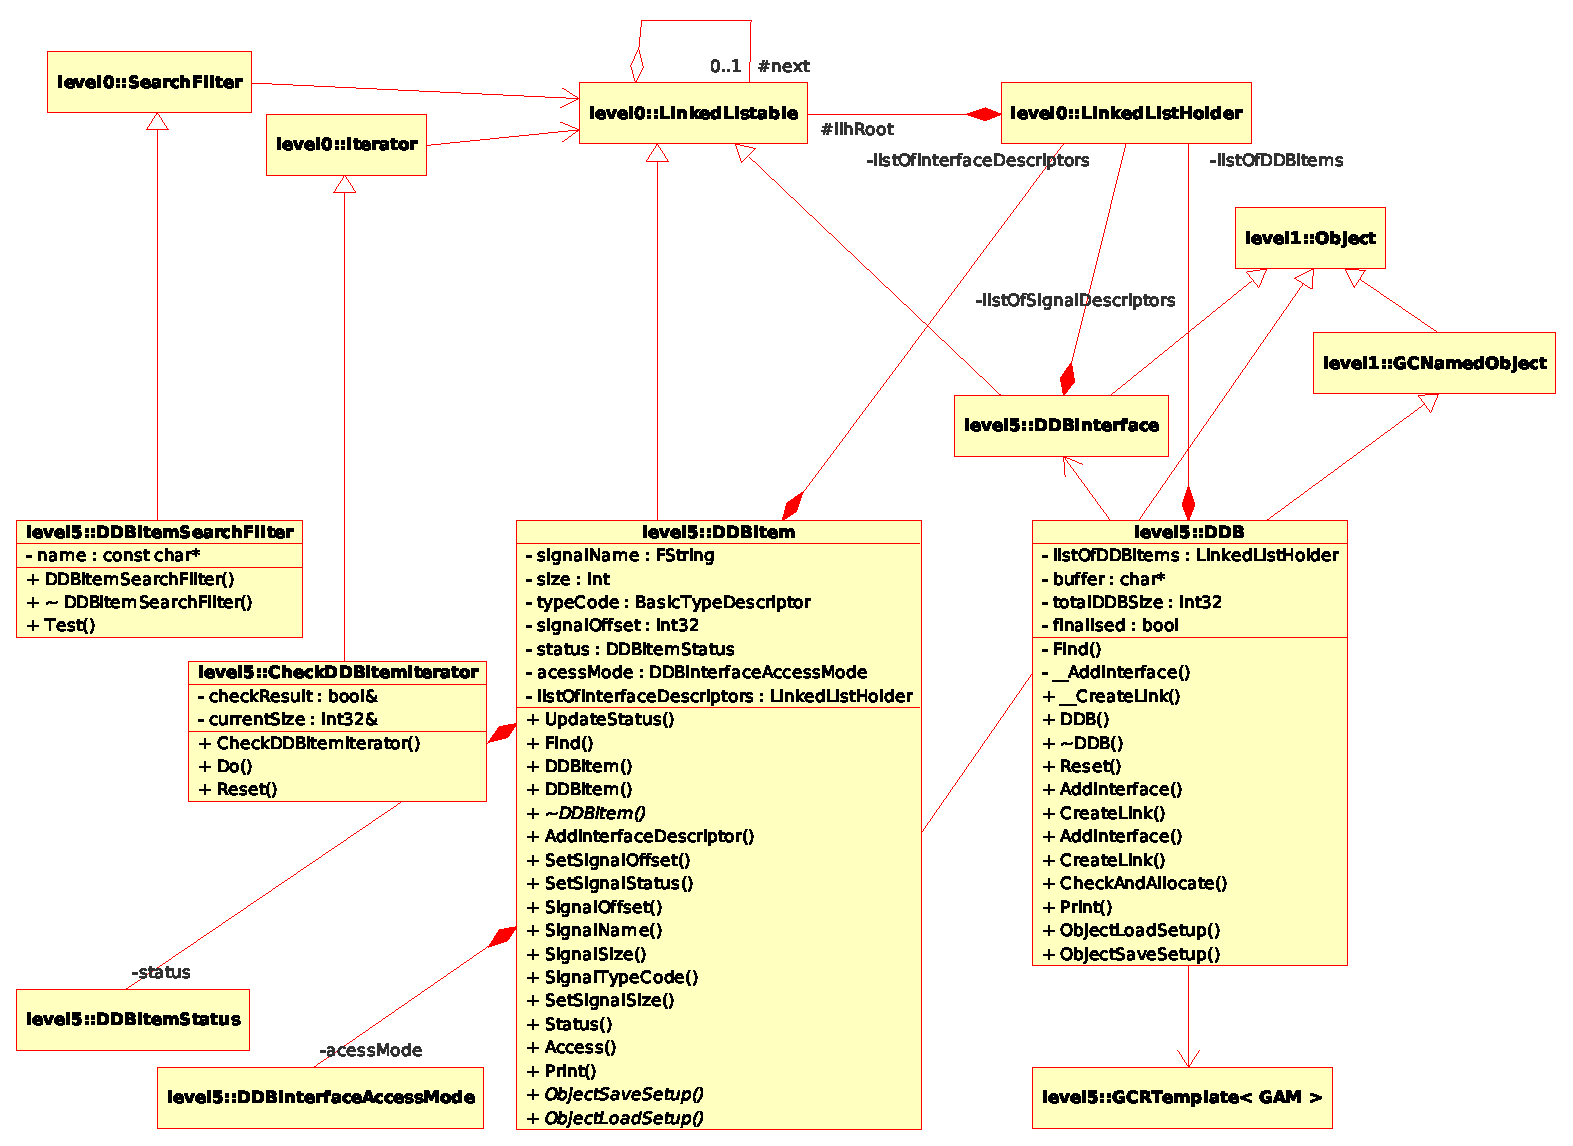
\includegraphics[width=\textwidth]{level5/level5-DDBItem.eps}
  \caption{BaseLib Level 5 DDBItem}
  \label{f:level5:DDBItem}
 \end{center}
\end{figure}

Classes involved in this section are depicted in Figure \ref{f:level5:DDBItem} and listed below:
\begin{itemize}
 \item DDBItemStatus
 \item DDBItem, CheckDDBItemIterator, DDBItemSearchFilter
 \item DDB
\end{itemize}



\subsubsection{DDBItemStatus}
\texttt{[DDBDefinitions.h, DDBDefinitions.cpp]}\\
The class \texttt{DDBItemStatus} is basically a variable (attribute \texttt{status}) coding the status of a \texttt{DDBItem}.
There are three constructors; the first one is the standard constructor that will be initialized the status to \texttt{OK} (or \texttt{DDB\_NoError}), the second is a constructor from integer, unfortunately is not possible to avoid usign it to make the constants. The third is a copy constructor.

Assignment operator, bitwise operators and the equal operator are redefined. The method \texttt{Check} check the object with the mask. \texttt{Print} method prints the mask.
\begin{lstlisting}[
extendedchars=true,%
basicstyle=\fontfamily{pcr}\fontseries{m}\selectfont\footnotesize, %
stepnumber=1,%
numberstyle=\tiny,%
keywordstyle=\footnotesize\tt ,%
language=C++]
   int status;
public:
   DDBItemStatus();
   DDBItemStatus(const int intStatus);
   DDBItemStatus(const DDBItemStatus& reference);

   DDBItemStatus& operator=(const DDBItemStatus right);
   DDBItemStatus& operator|=(const DDBItemStatus right);
   DDBItemStatus& operator&=(const DDBItemStatus right);
   DDBItemStatus operator~() const;
   bool operator==(const DDBItemStatus& reference) const;

   bool CheckMask(const DDBItemStatus& mask) const;
   void Print(StreamInterface& s) const;
\end{lstlisting}

In BaseLib are defined the following \texttt{DDBItemStatus}:

\begin{table}[!h]
 \begin{center}
  \begin{tabular}{|l|c|l|}
   \hline
type & value & description \\
   \hline
\texttt{DDB\_NoError} & 0x00 & The DDBItem status is OK. \\
\texttt{DDB\_WriteConflictError} & 0x01 & More than one user set as Writer on the signal. \\
\texttt{DDB\_WriteExclusiveViolation} & 0x02 & One or more user set as Patcher of a signal which is exclusively written by another user. \\
\texttt{DDB\_MissingSourceError} & 0x04 & The signal is read by a user but it is not written by any user. \\
\texttt{DDB\_ConsecutivityViolation} & 0x08 & It has not been possible to arrange the items in the DDB as requested by the consecutive bit. \\
\texttt{DDB\_SizeMismatch} & 0x10 & Set when a reader of a signal try to access it beyond the limit specified by the writer. \\
\texttt{DDB\_UndefinedSize} & 0x20 & Set when a signal is usized. \\
\texttt{DDB\_TypeMismatch} & 0x40 & Set when a mismatch between type is found. \\
\texttt{DDB\_UndefinedType} & 0x80 & Set when a mismatch between type is found. \\
   \hline
  \end{tabular}
 \end{center}
\end{table}



\subsubsection{DDBItem}
\texttt{[DDBItem.h, DDBItem.cpp]}\\
This class imlements the abstraction of the signal descriptor from the DDB point of view. The name of the \texttt{DDBItem} is the same as the name of the signal. It inherits from \texttt{LinkedListable} and \texttt{Object}. The attribute \texttt{signalName} is obviously the name of the signal. \texttt{size} is the size of the signal, \texttt{typeCode} is a field coding the type and size of the elementary type used to build this signal; \texttt{signalOffset} is the offset in bytes of the signal structure in the DBB. It will be set to 0 at construction time and updated by the proper function of the DDB class.
The attribute \texttt{status} contains the status of the signal (i.e. if there are some errors..).
The attribute \texttt{accessMode} contains the access mode of the signal (should be the or of the access modes of the DDB interfaces) and \texttt{listOfInterfaceDescriptors} is a list of users of the signal accounted by the \texttt{DDBItem}.

\begin{lstlisting}[
extendedchars=true,%
basicstyle=\fontfamily{pcr}\fontseries{m}\selectfont\footnotesize, %
stepnumber=1,%
numberstyle=\tiny,%
keywordstyle=\footnotesize\tt ,%
language=C++]
private:
   FString signalName;
   int size;
   BasicTypeDescriptor typeCode;
   int32 signalOffset;
   DDBItemStatus status;
   DDBInterfaceAccessMode accessMode;
   LinkedListHolder listOfInterfaceDescriptors;
\end{lstlisting}

The method \texttt{UpdateStatus} updates the status of the \texttt{DDBItem} after insertion of a new interface; the function checks whether there are some access violation and set the status accordingly.
The method \texttt{Find} finds by name a user (i.e. a \texttt{DDBInterfaceDescriptor}) in the \texttt{listOfInterfaceDescriptors}. \\


The method \texttt{AddInterfaceDescriptor} if it is the first user sets the variables name and type otherwise it checks for compatibility, it may set the \texttt{WriteConflictError} bit.
The method \texttt{SetSignalOffset} is basically used by the \texttt{AddInterface} method in DDB; \texttt{SetSignalStatus} sets the signal status to the desired value; previous values stored in the status are lost. \\


The method \texttt{SignalOffset} reads the \texttt{signalOffset} attribute; \texttt{SignalName} returns the \texttt{signalName}; \texttt{SignalSize} returns the signal size; \texttt{SignalTypeCode} returns the signal type code. The method \texttt{SetSignalSize} sets the signal size to the desired value. \texttt{Status} returns a copy of the \texttt{DDBItemStatus} attribute. \texttt{Access} returns a copy of the \texttt{DDBItemAccessMode} attribute. \texttt{Print} prints the object data. \\

The method \texttt{ObjectSaveSetup} uses a CDB to write the parameters, the CDB information is written to the subtree that is currently addressed. \texttt{ObjectLoadSetup} uses a CDB to pass the initialisation parameters, the CDB information is read from the subtree that is currently addressed.

\begin{lstlisting}[
extendedchars=true,%
basicstyle=\fontfamily{pcr}\fontseries{m}\selectfont\footnotesize, %
stepnumber=1,%
numberstyle=\tiny,%
keywordstyle=\footnotesize\tt ,%
language=C++]
private:
   void UpdateStatus(const DDBInterface& ddbInterface);
   DDBInterfaceDescriptor* Find(const DDBInterface& ddbInterface);

public:
   DDBItem(const char* signalName,int size,BasicTypeDescriptor typeCode);
   DDBItem(const DDBSignalDescriptor& descriptor);
   virtual ~DDBItem();

   bool AddInterfaceDescriptor(const DDBInterface& ddbInterface);
   void SetSignalOffset(int32 offset);

   void SetSignalStatus(DDBItemStatus status);
   int32 SignalOffset() const;
   const char* SignalName()const;

   int32 SignalSize();
   BasicTypeDescriptor SignalTypeCode() const;

   void SetSignalSize(int32 size);
   DDBItemStatus Status() const;
   DDBInterfaceAccessMode Access() const;
   void Print(StreamInterface& s, bool showUsers);

   virtual bool ObjectSaveSetup(ConfigurationDataBase& cdb,StreamInterface* err);
   virtual bool ObjectLoadSetup(ConfigurationDataBase& cdb,StreamInterface* err);
\end{lstlisting}



\subsubsection{CheckDDBItemIterator}
\texttt{[DDBItem.h, DDBItem.cpp]}\\
The class \texttt{CheckDDBItemIterator} is the iterator for a list of \texttt{DDBItem}; after the iterator has been used, a call to the \texttt{Reset} method need to be made to use it again.

The iterator has two attibutes, the first, \texttt{checkResult} is the result of of the check on the \texttt{DDBItem} list, the second, \texttt{currentSize} is the size of the required DDB space during the iteration of the list.

\begin{lstlisting}[
extendedchars=true,%
basicstyle=\fontfamily{pcr}\fontseries{m}\selectfont\footnotesize, %
stepnumber=1,%
numberstyle=\tiny,%
keywordstyle=\footnotesize\tt ,%
language=C++]
private:
   bool& checkResult;
   int32& currentSize;

public:
   CheckDDBItemIterator(bool& checkResult, int32& currentSize);

   void Do(LinkedListable* ll);
   void Reset();
\end{lstlisting}



\subsubsection{DDBItemSearchFilter}
\texttt{[DDBItem.h, DDBItem.cpp]}\\
This class implements the search of a \texttt{DDBItem} by name. It inherits as usal from the \texttt{SearchFilter} class. The attribute \texttt{name} is the string to search for.

\begin{lstlisting}[
extendedchars=true,%
basicstyle=\fontfamily{pcr}\fontseries{m}\selectfont\footnotesize, %
stepnumber=1,%
numberstyle=\tiny,%
keywordstyle=\footnotesize\tt ,%
language=C++]
private:
   const char* name;

public:
   DDBItemSearchFilter(const char* name);
   virtual ~DDBItemSearchFilter();

   bool Test(LinkedListable* ll);
\end{lstlisting}



\subsubsection{DDB}
\texttt{[DDB.h, DDB.cpp]}\\
The class \texttt{DDB} is \texttt{Dynamic Data Buffer} class definition, the DDB provides a way to store the signals in memory and made data exchange in Real Time. It inherits from \texttt{GCNamedObject}.

The attribute \texttt{listOfDDBItems} is a list of signal descriptions (\texttt{DDBItem} objects). The attribute \texttt{buffer} is a pointer to the buffer memory, \texttt{totalDDBSize} is the size in byte of the DDB buffer. The attribute \texttt{finalised} is a flag specifying if the DDB has been finalised, when the DDB is finalised it cannot accept new \texttt{DDBItem}s, the \texttt{CheckAndAllocate} method sets this flag if the DDB is coherent.

\begin{lstlisting}[
extendedchars=true,%
basicstyle=\fontfamily{pcr}\fontseries{m}\selectfont\footnotesize, %
stepnumber=1,%
numberstyle=\tiny,%
keywordstyle=\footnotesize\tt ,%
language=C++]
private:
   LinkedListHolder listOfDDBItems;

   char* buffer;
   int32 totalDDBSize;
   bool finalised;
\end{lstlisting}

The method \texttt{Find} finds a \texttt{DDBItem} by name in the \texttt{listOfDDBItems} list; the name of the \texttt{DDBItem} is the name of the signal has passed to the \texttt{DDBInterface}.
The method \texttt{\_\_AddInterface} is a private method that implements the public \texttt{AddInterface} method; the reason of this member is to allow access to private members of the \texttt{DDBInterface} from the exported functions.
The method \texttt{\_\_CreateLink} is a private member that implements the public \texttt{CreateLink} method, the reason of this member is to allow access to private members of the \texttt{DDBInterface} from the exported functions.\\


The method \texttt{AddInterface} is used to add an interface to the DDB. The method \texttt{CreateLink} can be used only if the DDB is finalised, a call to this method will initialise pointers (in the \texttt{DataBufferPointer} object) in the specified interface. The second method \texttt{AddInterface} is used to add all the interfaces that are used by a GAM to the DDB. The second declared method \texttt{CreateLink}, used after the DDB is finalised, will initialise pointers to all interfaces in the specified GAM. \\


The method \texttt{CheckAndAllocate} checks the list of \texttt{DDBItem} for consistency and allocates the memory. The method \texttt{Print} prints the DDB information on the specified stream.
The method \texttt{ObjectLoadSetup} loads the DDB parameters from the CDB and \texttt{ObjectSaveSetup} saves the DDB Parameters from the CDB.

\begin{lstlisting}[
extendedchars=true,%
basicstyle=\fontfamily{pcr}\fontseries{m}\selectfont\footnotesize, %
stepnumber=1,%
numberstyle=\tiny,%
keywordstyle=\footnotesize\tt ,%
language=C++]
   DDBItem* Find(const char* name);
   bool __AddInterface(const DDBInterface& gamInterface);
   bool __CreateLink(DDBInterface& gamInterface);

public:
   DDB();
   ~DDB();

   void Reset();
   bool AddInterface(const DDBInterface& gamInterface);
   bool CreateLink(DDBInterface& gamInterface);
   bool AddInterface(GCRTemplate<GAM> gam);
   bool CreateLink(GCRTemplate<GAM> gam);

   bool CheckAndAllocate();
   void Print(Streamable& s);

   bool ObjectLoadSetup(ConfigurationDataBase& cdb, StreamInterface* err);
   bool ObjectSaveSetup(ConfigurationDataBase& cdb, StreamInterface* err);
\end{lstlisting}



\subsection{Design Notes}
\texttt{ShowSignalDescriptorIterator} and \texttt{DDBSignalSearchFilter} (but also
\texttt{InterfaceDescriptorShowIterator} \texttt{DDBInterfaceDescriptorSearchFilteral}) use \texttt{dynamic\_cast} C++ operator that can throws exceptions, there is no code that catch those exceptions but only an if that checks against the zero value of this cast.

The following note is really important: using the GNU GCC compilers catching a \texttt{std::bad\_cast} exception is possible only if the conversion is done by reference and not by pointers. \\


The DDB doesn't provide access control to the differents memory area it provides. The concurrent access control to the areas must be done at higher level (MARTe). \\

\begin{figure}[h!]
 \begin{center}
  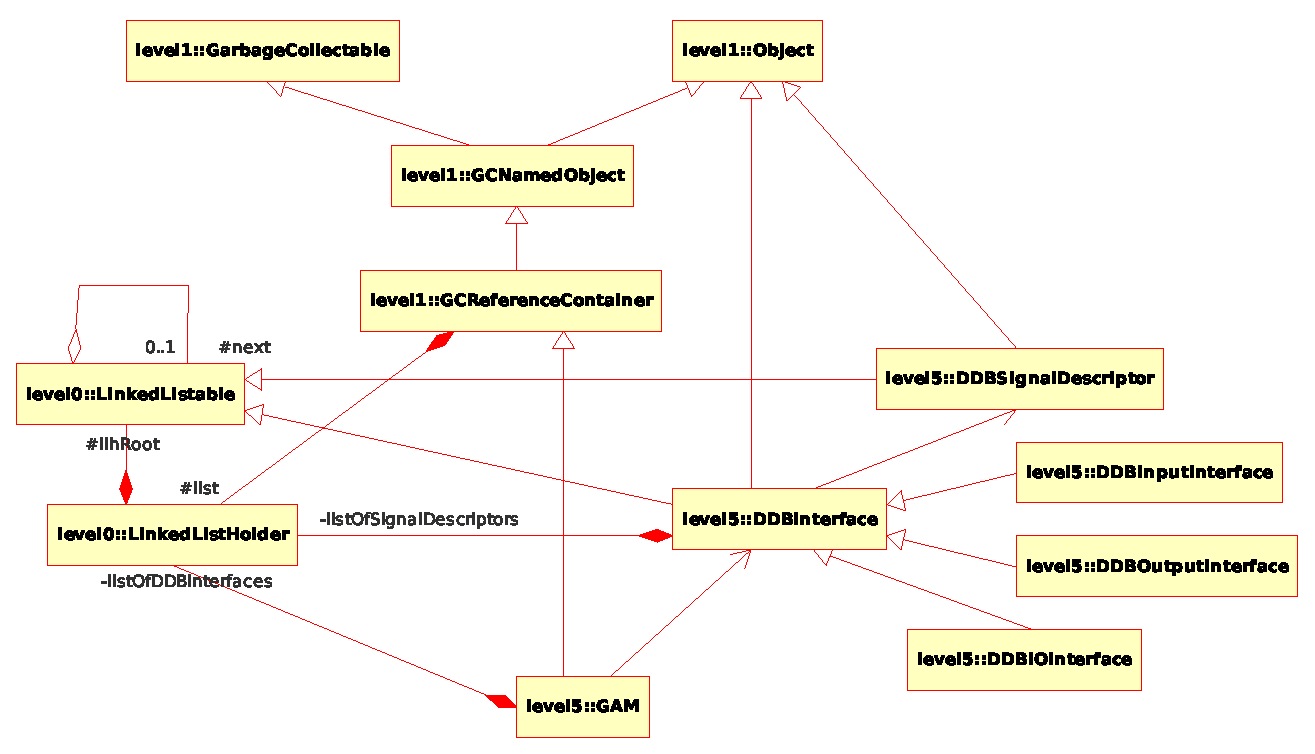
\includegraphics[width=0.91\textwidth]{level5/GAM.eps}
  \caption{BaseLib Level 5 GAM hierical in the DDB}
  \label{f:level5:GAM_GCReferenceContainer}
 \end{center}
\end{figure}

Looking at figure \ref{f:level5:GAM_GCReferenceContainer} you can see that GAM is a GCReferenceContainer, well, a GCReferenceContainer holds a LinkedListHolder as an attribute, GAM has another linked list holder as an attribute: GAM has two LinkedListHolder but it uses only one! On this LinkedListHolder it has DDBInterface elements that can be of input output or either.

Deepening in an implementation of a GAM when you use AddInputInterface (and others...) you are adding your Interface to the list and to another attribute you have to pass to the method. this attribute must be implemented in the new GAM.

Quindi crea un Linkedlist holder che tiene tutte le DDBinterface e ogni interfaccia deve pero essere puntata dall'interno della tua GAM di modo che ti obbliga cmq ad averne un controllo (per poterla anche usare nel codice). (penso che il puntatore all'interfaccia che hai nella classe non venga mai usato per avere array di interfaccie).



\section{Menu}
The menu infrastructure lets the user creating a menu structure with which is possible to navigate between menu entry and select a menu entry to execute. A menu structure can be created in C source code or via the wide used CDB. An excerpt of a menu created via the CDB follows. The example create a menu with two entry: one labelled ``Abort'' and another labelled ``Inhibit''. Each of those when selected sends a message.

\begin{lstlisting}[
extendedchars=true,%
basicstyle=\fontfamily{pcr}\fontseries{m}\selectfont\footnotesize, %
stepnumber=1,%
numberstyle=\tiny,%
keywordstyle=\footnotesize\tt ,%
language=bash]
+MARTeMenu = {
    Class = MARTeMenu
    Title = "MARTe Menu"
    +MenuA = {
        Class = MenuContainer
        Title = "CODAS Interface"
        +ABORT = {
            Class = SendMessageMenuEntry
            Title = Abort
            Envelope = {
               ...
            }
        }
        +INHIBIT = {
            Class = SendMessageMenuEntry
            Title = Inhibit
            Envelope = {
                Class = MessageEnvelope
                Sender = MARTeMenu
                Destination = StateMachine
                +Message = {
                    Class = Message
                    Code = 0x704
                    Content = Inhibit
                }
            }
        }
        ...
    }
    ...
}
\end{lstlisting}

\begin{figure}[h!]
 \begin{center}
  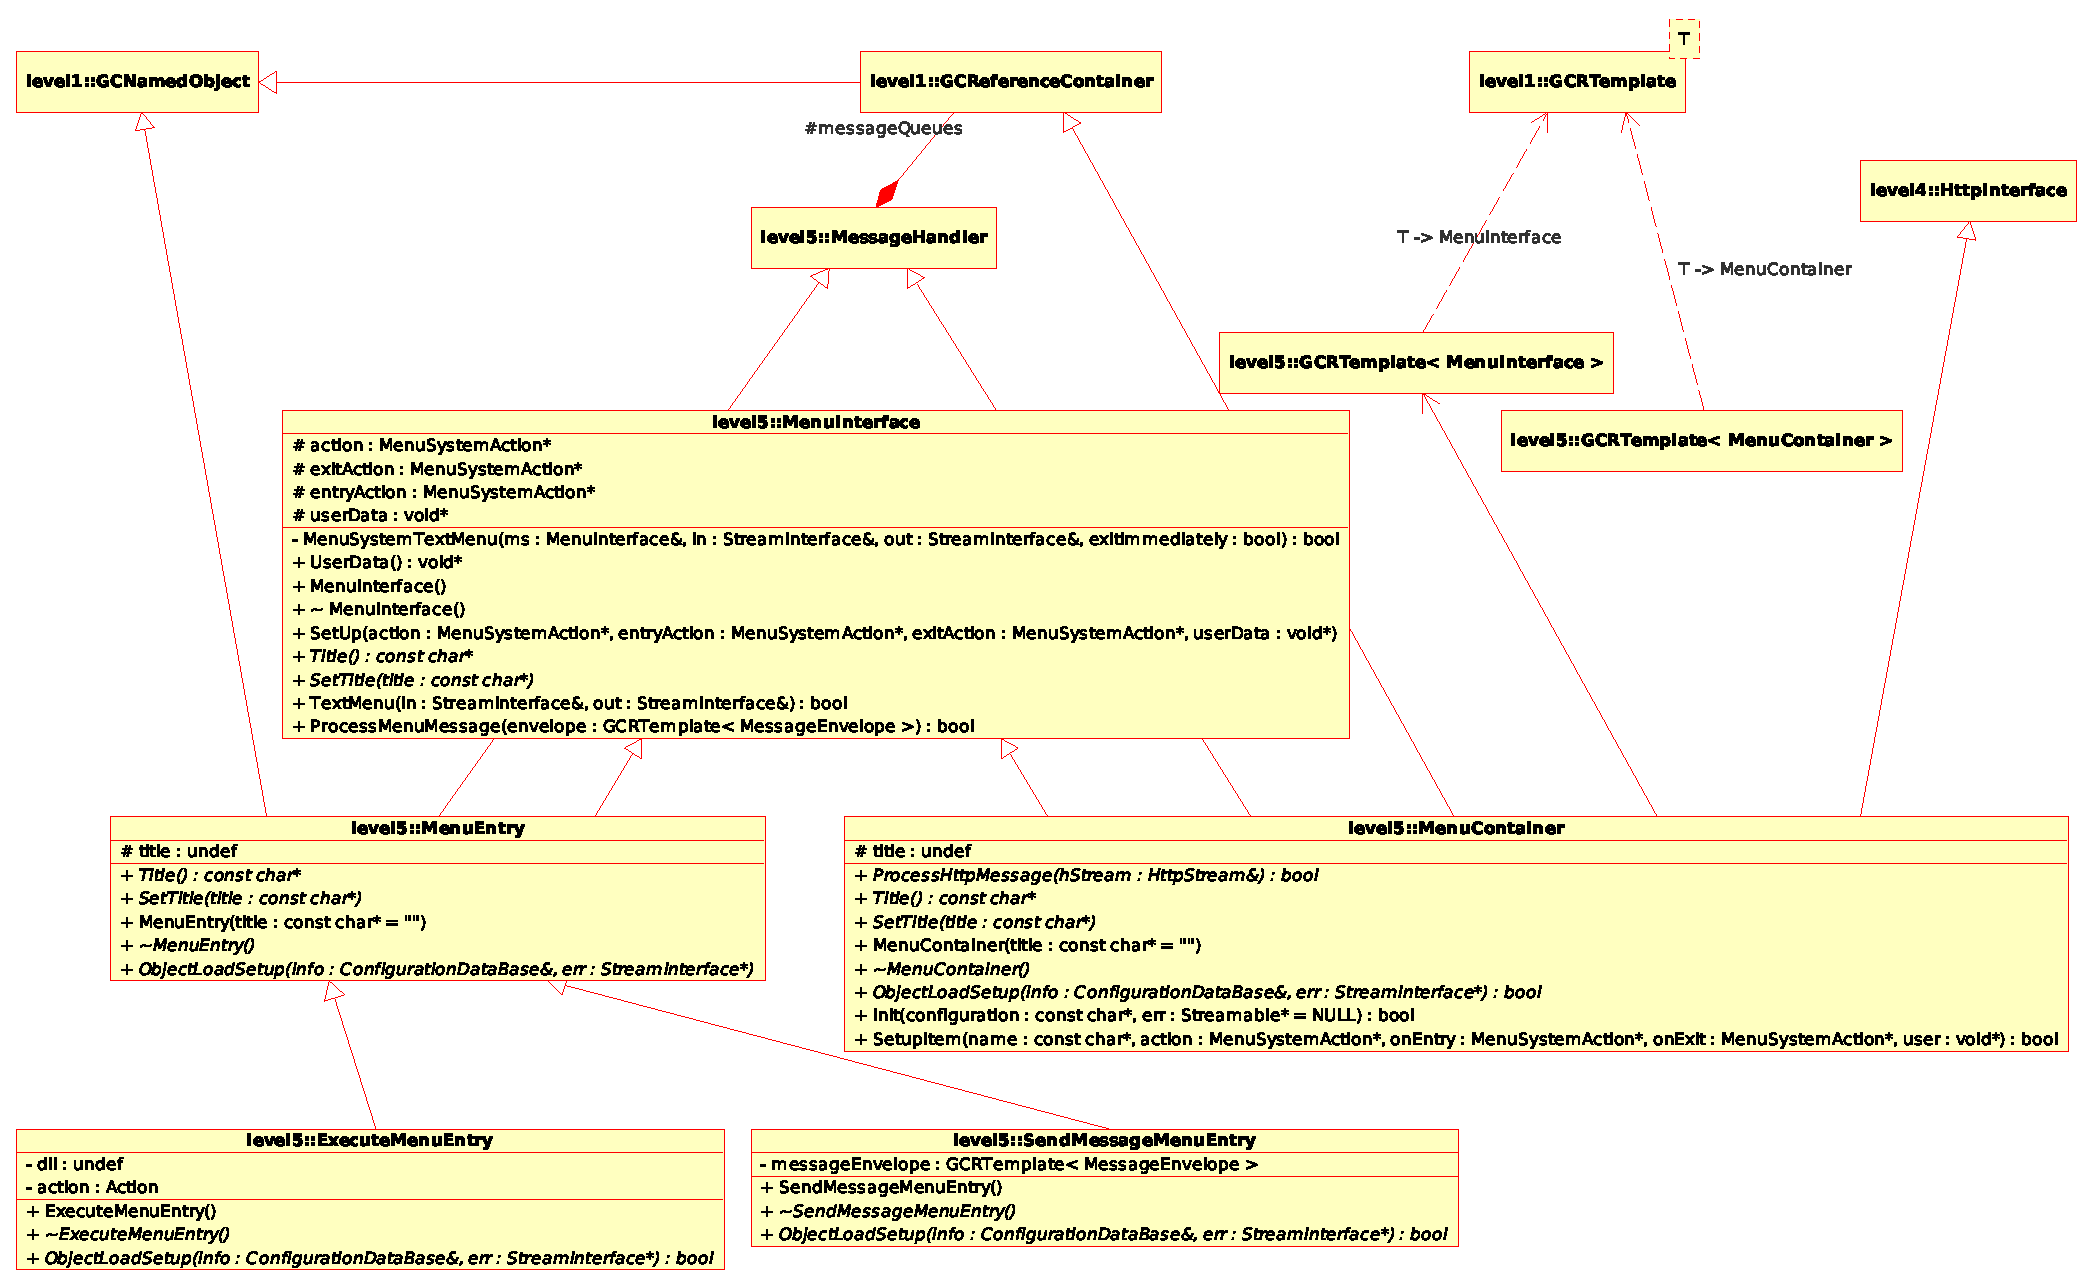
\includegraphics[width=\textwidth]{level5/level5-Menu-exp.eps}
  \caption{BaseLib Level 5 Menu}
  \label{f:level5:Menu}
 \end{center}
\end{figure}

Classes involved in this section are depicted in Figure \ref{f:level5:Menu} and listed below:
\begin{itemize}
 \item MenuInterface
 \item MenuEntry
 \item ExecuteMenuEntry
 \item SendMessageMenuEntry
 \item MenuContainer
\end{itemize}



\subsubsection{MenuInterface}
\texttt{[MenuInterface.h, MenuInterface.cpp]}\\
The class \texttt{MenuInterface} starts with a prototype for a function to associate to a menu page, it follows.

\begin{lstlisting}[
extendedchars=true,%
basicstyle=\fontfamily{pcr}\fontseries{m}\selectfont\footnotesize, %
stepnumber=1,%
numberstyle=\tiny,%
keywordstyle=\footnotesize\tt ,%
language=C++]
typedef bool (MenuSystemAction)(StreamInterface& in,StreamInterface& out,void* userData);
\end{lstlisting}

Such function takes as parameters an input straem, an output stream and a pointer to user data.
The class \texttt{MenuInterface} is used to build a tree or menu pages that operate via the \texttt{StreamInterface}.
The first \texttt{MenuSystemAction*} attribute define an action, if this is not NULL this is a menu container. The second attribute define an action to do when exiting and the last \texttt{MenuSystemAction*} let you set what to do before entering the menu item. The attribute \texttt{userData} contains user specific information, that can be retrieved using the \texttt{UserData} method. \\


The method \texttt{SetUp} sets the action associated with this menu item, the pure virtual method \texttt{Title} is defined to be able to choose the labelling policy and returns the label of the menu that can be set with \texttt{SetTitle}. The method \texttt{TextMenu} calls the menu and \texttt{PRocessMenuMessage} is called by a class if it is also a \texttt{MessageHandler}.
\begin{lstlisting}[
extendedchars=true,%
basicstyle=\fontfamily{pcr}\fontseries{m}\selectfont\footnotesize, %
stepnumber=1,%
numberstyle=\tiny,%
keywordstyle=\footnotesize\tt ,%
language=C++]
protected:
   MenuSystemAction* action;
   MenuSystemAction* exitAction;
   MenuSystemAction* entryAction;

   void* userData;
public:
   void* UserData();

public:
   MenuInterface();
   virtual ~MenuInterface();

   void SetUp(MenuSystemAction* action,MenuSystemAction* entryAction,
      MenuSystemAction* exitAction,void* userData);
   virtual const char* Title()=0;
   virtual void SetTitle(const char* title)=0;

   virtual bool TextMenu(StreamInterface& in,StreamInterface& out);
   bool ProcessMenuMessage(GCRTemplate<MessageEnvelope> envelope);
\end{lstlisting}



\subsubsection{MenuEntry}
\texttt{[MenuEntry.h, MenuEntry.cpp]}\\
The class \texttt{MenuEntry} is used to build a tree o menu pages that operate via Streamable. It inherits from \texttt{MenuInterface}, \texttt{MessageHandler} and \texttt{GCNamedObject} so it is a menu part that can handle messages and it is garbage collectable and addressable by name.

It implements the pure virtual methods of \texttt{MenuInterface} infact it has one \texttt{BString} attribute as a \texttt{title}, distinct from the object name.

The method \texttt{ObjectLoadSetup} create a tree of \texttt{MenuContainer} and \texttt{MenuEntry} from a CDB, it search the CDB for \texttt{Title} entry.

\begin{lstlisting}[
extendedchars=true,%
basicstyle=\fontfamily{pcr}\fontseries{m}\selectfont\footnotesize, %
stepnumber=1,%
numberstyle=\tiny,%
keywordstyle=\footnotesize\tt ,%
language=C++]
protected:
   BString title;

public:
   virtual const char* Title()
   virtual void SetTitle(const char* title)

   MenuEntry(const char* title= "")
   virtual ~MenuEntry()

   virtual bool ObjectLoadSetup(ConfigurationDataBase& info,StreamInterface* err);
\end{lstlisting}



\subsubsection{ExecuteMenuEntry}
\texttt{[ExecuteMenuEntry.h, ExecuteMenuEntry.cpp]}\\
The class \texttt{ExecuteMenutEntry} starts defining the following type:

\begin{lstlisting}[
extendedchars=true,%
basicstyle=\fontfamily{pcr}\fontseries{m}\selectfont\footnotesize, %
stepnumber=1,%
numberstyle=\tiny,%
keywordstyle=\footnotesize\tt ,%
language=C++]
typedef bool (*Action)(StreamInterface& in,StreamInterface& out,void* userData);
\end{lstlisting}

Such class inherits from \texttt{MenuEntry} so has all the same capability and adds an action.
The \texttt{LoadableLibrary} attribute is a user specified DLL containing the function to be executed and \texttt{action} is a pointer to the user specified action.

\begin{lstlisting}[
extendedchars=true,%
basicstyle=\fontfamily{pcr}\fontseries{m}\selectfont\footnotesize, %
stepnumber=1,%
numberstyle=\tiny,%
keywordstyle=\footnotesize\tt ,%
language=C++]
private:
   LoadableLibrary dll;
   Action action;

public:
   ExecuteMenuEntry();
   virtual ~ExecuteMenuEntry();

   virtual bool ObjectLoadSetup(ConfigurationDataBase& info,StreamInterface* err);
\end{lstlisting}



\subsubsection{SendMessageMenuEntry}
\texttt{[SendMessageMenuEntry.h, SendMessageMenuEntry.cpp]}\\
The class \texttt{SendMessageMenuEntry} is a \texttt{MenuEntry} object that contains a \texttt{MessageEnvelope} used for sending a message. This \texttt{MenuEntry} class is able to react when selected sending a message.

The method \texttt{ObjectLoadSetup} calls the \texttt{MenuEntry}'s \texttt{ObjectLoadSetup} and then loads the user specified \texttt{MessageEnvelope} according to the \texttt{MessageEnvelope} specifications. The \texttt{MessageEnvelope} must be specified within a member named \texttt{Envelope}.
 
\begin{lstlisting}[
extendedchars=true,%
basicstyle=\fontfamily{pcr}\fontseries{m}\selectfont\footnotesize, %
stepnumber=1,%
numberstyle=\tiny,%
keywordstyle=\footnotesize\tt ,%
language=C++]
private:
   GCRTemplate<MessageEnvelope> messageEnvelope;

public:
   SendMessageMenuEntry();
   virtual ~SendMessageMenuEntry(){}

   virtual bool ObjectLoadSetup(ConfigurationDataBase& info,StreamInterface* err);
\end{lstlisting}



\subsubsection{MenuContainer}
\texttt{[MenuContainer.h, MenuContainer.cpp]}\\
A \texttt{MenuContainer} class is a container of \texttt{MenuEntry} objects, it inherits infact from \texttt{GCReferenceContainer}; it inherits also from \texttt{MenuInterface}, \texttt{MessageHandler} and \texttt{HttpInterface}.

The only attribute, like \texttt{MenuEntry}, is \texttt{title}, i.e. a specific title, distinct from the object name; \texttt{title} can be returned using \texttt{Title} and setted by \texttt{SetTitle} method. The method \texttt{ProcessHttpMessage} is the main entry point for \texttt{HttpInterface}. \\


The method \texttt{ObjectLoadSetup} use the initialization syntax of \texttt{GCReferenceContainer}, additionally set the \texttt{title}; using the above mentioned syntax it is possible to create a tree of \texttt{MenuContainer} and \texttt{MenuEntry} that individually access the \texttt{MenuEntry} elements to set the user functions.
The method \texttt{Init} creates a menu tree creating a stream first then a CDB and then using \texttt{ObjectLoadSetup}. \texttt{SetupItem} allows setting up the user functions and data for a specific sub menu, the menu is identified by the path to reach the specific menu item.

\begin{lstlisting}[
extendedchars=true,%
basicstyle=\fontfamily{pcr}\fontseries{m}\selectfont\footnotesize, %
stepnumber=1,%
numberstyle=\tiny,%
keywordstyle=\footnotesize\tt ,%
language=C++]
protected:
   BString title;

public:
   virtual const char* Title();
   virtual void SetTitle(const char* title);
   virtual bool ProcessHttpMessage(HttpStream &hStream);

   MenuContainer(const char* title="");
   virtual ~MenuContainer();

   virtual bool ObjectLoadSetup(ConfigurationDataBase& info,StreamInterface* err);

   bool Init(const char* configuration,Streamable* err=NULL);
   bool SetupItem(const char* name,MenuSystemAction* action,MenuSystemAction* entryAction,
      MenuSystemAction* exitAction,void* userData);
\end{lstlisting}



\subsection{Design Notes}
A menu infrastructure is basically a tree where each leaf is an executable menu entry, i.e. if selected has associated a menu action to it. All this structure can be simplified implemented at lower level a tree data structure instead using list and sublists. This can lead to faster data structures.



\section{Other}


\subsubsection{HRT Synchronizer}
\texttt{[HRTSynchronised.h]}\\
This class depends only on \textit{level0/HRT.h} and \texttt{level0/HRT.cpp} nothing else is required to compile it, the class can be easily moved to \textit{level0}.\\


The first attribute, \texttt{oldTime} is a reference time of the previous call to the \texttt{Syncronise} method. The attribute \texttt{oldHrt} is the HRT value at the time of the previous call to the \texttt{Synchronise} method.

\texttt{hrtPeriod} is the current estimate of the HRT clock period, \texttt{timeOffset} is the offset used to calculate the time estimation and \texttt{lastTimeOffset} is another offset used to calculate the time estimation. \\


The method \texttt{Synchronise} must be called periodically to synchronise the current thread, this routine needs to be called at least 3 times before the class can be used (this is because it must aligns its offsets).
The method \texttt{Period} estimates the HRT period, the estimation is done using the external source.
The method \texttt{CurrentTime} returns the estimated time in seconds reading from the HRT timer.
\begin{lstlisting}[
extendedchars=true,%
basicstyle=\fontfamily{pcr}\fontseries{m}\selectfont\footnotesize, %
stepnumber=1,%
numberstyle=\tiny,%
keywordstyle=\footnotesize\tt ,%
language=C++]
private:
   double oldTime;
   int64 oldHrt;
   double hrtPeriod;
   double timeOffset;
   double lastTimeOffset;

public:
   HRTSynchronised();

   void Synchronise(int64 usecTime);
   double Period();
   double CurrentTime();
\end{lstlisting}



\subsection{Design Note}
The class \texttt{HRTSynchronised} depends only on \textit{level0/HRT.h} and \texttt{level0/HRT.cpp} nothing else is required to compile it, the class can be easily moved to \textit{level0}.


